%% bare_jrnl.tex
%% V1.4
%% 2012/12/27
%% by Michael Shell
%% see http://www.michaelshell.org/
%% for current contact information.
%%
%% This is a skeleton file demonstrating the use of IEEEtran.cls
%% (requires IEEEtran.cls version 1.8 or later) with an IEEE journal paper.
%%	
%% Support sites:
%% http://www.michaelshell.org/tex/ieeetran/
%% http://www.ctan.org/tex-archive/macros/latex/contrib/IEEEtran/
%% and
%% http://www.ieee.org/



% *** Authors should verify (and, if needed, correct) their LaTeX system  ***
% *** with the testflow diagnostic prior to trusting their LaTeX platform ***
% *** with production work. IEEE's font choices can trigger bugs that do  ***
% *** not appear when using other class files.                            ***
% The testflow support page is at:
% http://www.michaelshell.org/tex/testflow/

\def\eg{{e.g. }}
\def\etal{{et al. }}
\def\etc{{etc. }}
\def\ie{{i.e. }}
\newcommand{\ignore}[1]{}
%%*************************************************************************
%% Legal Notice:
%% This code is offered as-is without any warranty either expressed or
%% implied; without even the implied warranty of MERCHANTABILITY or
%% FITNESS FOR A PARTICULAR PURPOSE! 
%% User assumes all risk.
%% In no event shall IEEE or any contributor to this code be liable for
%% any damages or losses, including, but not limited to, incidental,
%% consequential, or any other damages, resulting from the use or misuse
%% of any information contained here.
%%
%% All comments are the opinions of their respective authors and are not
%% necessarily endorsed by the IEEE.
%%
%% This work is distributed under the LaTeX Project Public License (LPPL)
%% ( http://www.latex-project.org/ ) version 1.3, and may be freely used,
%% distributed and modified. A copy of the LPPL, version 1.3, is included
%% in the base LaTeX documentation of all distributions of LaTeX released
%% 2003/12/01 or later.
%% Retain all contribution notices and credits.
%% ** Modified files should be clearly indicated as such, including  **
%% ** renaming them and changing author support contact information. **
%%
%% File list of work: IEEEtran.cls, IEEEtran_HOWTO.pdf, bare_adv.tex,
%%                    bare_conf.tex, bare_jrnl.tex, bare_jrnl_compsoc.tex,
%%                    bare_jrnl_transmag.tex
%%*************************************************************************

% Note that the a4paper option is mainly intended so that authors in
% countries using A4 can easily print to A4 and see how their papers will
% look in print - the typesetting of the document will not typically be
% affected with changes in paper size (but the bottom and side margins will).
% Use the testflow package mentioned above to verify correct handling of
% both paper sizes by the user's LaTeX system.
%
% Also note that the "draftcls" or "draftclsnofoot", not "draft", option
% should be used if it is desired that the figures are to be displayed in
% draft mode.
%
\documentclass[journal]{IEEEtran}
%
% If IEEEtran.cls has not been installed into the LaTeX system files,
% manually specify the path to it like:
% \documentclass[journal]{../sty/IEEEtran}





% Some very useful LaTeX packages include:
% (uncomment the ones you want to load)


% *** MISC UTILITY PACKAGES ***
%
%\usepackage{ifpdf}
% Heiko Oberdiek's ifpdf.sty is very useful if you need conditional
% compilation based on whether the output is pdf or dvi.
% usage:
% \ifpdf
%   % pdf code
% \else
%   % dvi code
% \fi
% The latest version of ifpdf.sty can be obtained from:
% http://www.ctan.org/tex-archive/macros/latex/contrib/oberdiek/
% Also, note that IEEEtran.cls V1.7 and later provides a builtin
% \ifCLASSINFOpdf conditional that works the same way.
% When switching from latex to pdflatex and vice-versa, the compiler may
% have to be run twice to clear warning/error messages.






% *** CITATION PACKAGES ***
%
%\usepackage{cite}
% cite.sty was written by Donald Arseneau
% V1.6 and later of IEEEtran pre-defines the format of the cite.sty package
% \cite{} output to follow that of IEEE. Loading the cite package will
% result in citation numbers being automatically sorted and properly
% "compresseq:form_kerneled/ranged". e.g., [1], [9], [2], [7], [5], [6] without using
% cite.sty will become [1], [2], [5]--[7], [9] using cite.sty. cite.sty's
% \cite will automatically add leading space, if needed. Use cite.sty's
% noadjust option (cite.sty V3.8 and later) if you want to turn this off
% such as if a citation ever needs to be enclosed in parenthesis.
% cite.sty is already installed on most LaTeX systems. Be sure and use
% version 4.0 (2003-05-27) and later if using hyperref.sty. cite.sty does
% not currently provide for hyperlinked citations.
% The latest version can be obtained at:
% http://www.ctan.org/tex-archive/macros/latex/contrib/cite/
% The documentation is contained in the cite.sty file itself.






% *** GRAPHICS RELATED PACKAGES ***
%
\ifCLASSINFOpdf
  % \usepackage[pdftex]{graphicx}
  % declare the path(s) where your graphic files are
  % \graphicspath{{../pdf/}{../jpeg/}}
  % and their extensions so you won't have to specify these with
  % every instance of \includegraphics
  % \DeclareGraphicsExtensions{.pdf,.jpeg,.png}
\else
  % or other class option (dvipsone, dvipdf, if not using dvips). graphicx
  % will default to the driver specified in the system graphics.cfg if no
  % driver is specified.
  % \usepackage[dvips]{graphicx}
  % declare the path(s) where your graphic files are
  % \graphicspath{{../eps/}}
  % and their extensions so you won't have to specify these with
  % every instance of \includegraphics
  % \DeclareGraphicsExtensions{.eps}
\fi
% graphicx was written by David Carlisle and Sebastian Rahtz. It is
% required if you want graphics, photos, etc. graphicx.sty is already
% installed on most LaTeX systems. The latest version and documentation
% can be obtained at: 
% http://www.ctan.org/tex-archive/macros/latex/required/graphics/
% Another good source of documentation is "Using Imported Graphics in
% LaTeX2e" by Keith Reckdahl which can be found at:
% http://www.ctan.org/tex-archive/info/epslatex/
%
% latex, and pdflatex in dvi mode, support graphics in encapsulated
% postscript (.eps) format. pdflatex in pdf mode supports graphics
% in .pdf, .jpeg, .png and .mps (metapost) formats. Users should ensure
% that all non-photo figures use a vector format (.eps, .pdf, .mps) and
% not a bitmapped formats (.jpeg, .png). IEEE frowns on bitmapped formats
% which can result in "jaggedy"/blurry rendering of lines and letters as
% well as large increases in file sizes.
%
% You can find documentation about the pdfTeX application at:
% http://www.tug.org/applications/pdftex





% *** MATH PACKAGES ***
%
%\usepackage[cmex10]{amsmath}
% A popular package from the American Mathematical Society that provides
% many useful and powerful commands for dealing with mathematics. If using
% it, be sure to load this package with the cmex10 option to ensure that
% only type 1 fonts will utilized at all point sizes. Without this option,
% it is possible that some math symbols, particularly those within
% footnotes, will be rendered in bitmap form which will result in a
% document that can not be IEEE Xplore compliant!
%
% Also, note that the amsmath package sets \interdisplaylinepenalty to 10000
% thus preventing page breaks from occurring within multiline equations. Use:
%\interdisplaylinepenalty=2500
% after loading amsmath to restore such page breaks as IEEEtran.cls normally
% does. amsmath.sty is already installed on most LaTeX systems. The latest
% version and documentation can be obtained at:
% http://www.ctan.org/tex-archive/macros/latex/required/amslatex/math/





% *** SPECIALIZED LIST PACKAGES ***
%
%\usepackage{algorithmic}
% algorithmic.sty was written by Peter Williams and Rogerio Brito.
% This package provides an algorithmic environment fo describing algorithms.
% You can use the algorithmic environment in-text or within a figure
% environment to provide for a floating algorithm. Do NOT use the algorithm
% floating environment provided by algorithm.sty (by the same authors) or
% algorithm2e.sty (by Christophe Fiorio) as IEEE does not use dedicated
% algorithm float types and packages that provide these will not provide
% correct IEEE style captions. The latest version and documentation of
% algorithmic.sty can be obtained at:
% http://www.ctan.org/tex-archive/macros/latex/contrib/algorithms/
% There is also a support site at:
% http://algorithms.berlios.de/index.html
% Also of interest may be the (relatively newer and more customizable)
% algorithmicx.sty package by Szasz Janos:
% http://www.ctan.org/tex-archive/macros/latex/contrib/algorithmicx/




% *** ALIGNMENT PACKAGES ***
%
%\usepackage{array}
% Frank Mittelbach's and David Carlisle's array.sty patches and improves
% the standard LaTeX2e array and tabular environments to provide better
% appearance and additional user controls. As the default LaTeX2e table
% generation code is lacking to the point of almost being broken with
% respect to the quality of the end results, all users are strongly
% advised to use an enhanced (at the very least that provided by array.sty)
% set of table tools. array.sty is already installed on most systems. The
% latest version and documentation can be obtained at:
% http://www.ctan.org/tex-archive/macros/latex/required/tools/


% IEEEtran contains the IEEEeqnarray family of commands that can be used to
% generate multiline equations as well as matrices, tables, etc., of high
% quality.




% *** SUBFIGURE PACKAGES ***
%\ifCLASSOPTIONcompsoc
%  \usepackage[caption=false,font=normalsize,labelfont=sf,textfont=sf]{subfig}
%\else
%  \usepackage[caption=false,font=footnotesize]{subfig}
%\fi
% subfig.sty, written by Steven Douglas Cochran, is the modern replacement
% for subfigure.sty, the latter of which is no longer maintained and is
% incompatible with some LaTeX packages including fixltx2e. However,
% subfig.sty requires and automatically loads Axel Sommerfeldt's caption.sty
% which will override IEEEtran.cls' handling of captions and this will result
% in non-IEEE style figure/table captions. To prevent this problem, be sure
% and invoke subfig.sty's "caption=false" package option (available since
% subfig.sty version 1.3, 2005/06/28) as this is will preserve IEEEtran.cls
% handling of captions.
% Note that the Computer Society format requires a larger sans serif font
% than the serif footnote size font used in traditional IEEE formatting
% and thus the need to invoke different subfig.sty package options depending
% on whether compsoc mode has been enabled.
%
% The latest version and documentation of subfig.sty can be obtained at:
% http://www.ctan.org/tex-archive/macros/latex/contrib/subfig/




% *** FLOAT PACKAGES ***
%
%\usepackage{fixltx2e}
% fixltx2e, the successor to the earlier fix2col.sty, was written by
% Frank Mittelbach and David Carlisle. This package corrects a few problems
% in the LaTeX2e kernel, the most notable of which is that in current
% LaTeX2e releases, the ordering of single and double column floats is not
% guaranteed to be preserved. Thus, an unpatched LaTeX2e can allow a
% single column figure to be placed prior to an earlier double column
% figure. The latest version and documentation can be found at:
% http://www.ctan.org/tex-archive/macros/latex/base/


%\usepackage{stfloats}
% stfloats.sty was written by Sigitas Tolusis. This package gives LaTeX2e
% the ability to do double column floats at the bottom of the page as well
% as the top. (e.g., "\begin{figure*}[!b]" is not normally possible in
% LaTeX2e). It also provides a command:
%\fnbelowfloat
% to enable the placement of footnotes below bottom floats (the standard
% LaTeX2e kernel puts them above bottom floats). This is an invasive package
% which rewrites many portions of the LaTeX2e float routines. It may not work
% with other packages that modify the LaTeX2e float routines. The latest
% version and documentation can be obtained at:
% http://www.ctan.org/tex-archive/macros/latex/contrib/sttools/
% Do not use the stfloats baselinefloat ability as IEEE does not allow
% \baselineskip to stretch. Authors submitting work to the IEEE should note
% that IEEE rarely uses double column equations and that authors should try
% to avoid such use. Do not be tempted to use the cuted.sty or midfloat.sty
% packages (also by Sigitas Tolusis) as IEEE does not format its papers in
% such ways.
% Do not attempt to use stfloats with fixltx2e as they are incompatible.
% Instead, use Morten Hogholm'a dblfloatfix which combines the features
% of both fixltx2e and stfloats:
%
% \usepackage{dblfloatfix}
% The latest version can be found at:
% http://www.ctan.org/tex-archive/macros/latex/contrib/dblfloatfix/




%\ifCLASSOPTIONcaptionsoff
%  \usepackage[nomarkers]{endfloat}
% \let\MYoriglatexcaption\caption
% \renewcommand{\caption}[2][\relax]{\MYoriglatexcaption[#2]{#2}}
%\fi
% endfloat.sty was written by James Darrell McCauley, Jeff Goldberg and 
% Axel Sommerfeldt. This package may be useful when used in conjunction with 
% IEEEtran.cls'  captionsoff option. Some IEEE journals/societies require that
% submissions have lists of figures/tables at the end of the paper and that
% figures/tables without any captions are placed on a page by themselves at
% the end of the document. If needed, the draftcls IEEEtran class option or
% \CLASSINPUTbaselinestretch interface can be used to increase the line
% spacing as well. Be sure and use the nomarkers option of endfloat to
% prevent endfloat from "marking" where the figures would have been placed
% in the text. The two hack lines of code above are a slight modification of
% that suggested by in the endfloat docs (section 8.4.1) to ensure that
% the full captions always appear in the list of figures/tables - even if
% the user used the short optional argument of \caption[]{}.
% IEEE papers do not typically make use of \caption[]'s optional argument,
% so this should not be an issue. A similar trick can be used to disable
% captions of packages such as subfig.sty that lack options to turn off
% the subcaptions:
% For subfig.sty:
% \let\MYorigsubfloat\subfloat
% \renewcommand{\subfloat}[2][\relax]{\MYorigsubfloat[]{#2}}
% However, the above trick will not work if both optional arguments of
% the \subfloat command are used. Furthermore, there needs to be a
% description of each subfigure *somewhere* and endfloat does not add
% subfigure captions to its list of figures. Thus, the best approach is to
% avoid the use of subfigure captions (many IEEE journals avoid them anyway)
% and instead reference/explain all the subfigures within the main caption.
% The latest version of endfloat.sty and its documentation can obtained at:
% http://www.ctan.org/tex-archive/macros/latex/contrib/endfloat/
%
% The IEEEtran \ifCLASSOPTIONcaptionsoff conditional can also be used
% later in the document, say, to conditionally put the References on a 
% page by themselves.




% *** PDF, URL AND HYPERLINK PACKAGES ***
%
%\usepackage{url}
% url.sty was written by Donald Arseneau. It provides better support for
% handling and breaking URLs. url.sty is already installed on most LaTeX
% systems. The latest version and documentation can be obtained at:
% http://www.ctan.org/tex-archive/macros/latex/contrib/url/
% Basically, \url{my_url_here}.




% *** Do not adjust lengths that control margins, column widths, etc. ***
% *** Do not use packages that alter fonts (such as pslatex).         ***
% There should be no need to do such things with IEEEtran.cls V1.6 and later.
% (Unless specifically asked to do so by the journal or conference you plan
% to submit to, of course. )


% correct bad hyphenation here
\hyphenation{op-tical net-works semi-conduc-tor}

\usepackage{url}

\usepackage{times}
\usepackage{epsfig}
%\usepackage{graphicx}
\usepackage{graphicx,dblfloatfix}
\usepackage{amsmath}
\usepackage{amssymb}
\usepackage{comment}
\usepackage{booktabs}
\usepackage{caption}
\usepackage{subcaption}
\usepackage{array}
\graphicspath{{./figures/}}


\usepackage{expl3}
\ExplSyntaxOn
\newcommand\latinabbrev[1]{
  \peek_meaning:NTF . {% Same as \@ifnextchar
    #1\@}%
  { \peek_catcode:NTF a {% Check whether next char has same catcode as \'a, i.e., is a letter
      #1.\@ }%
    {#1.\@}}}
\ExplSyntaxOff

%Omit final dot from each def.
\def\eg{\latinabbrev{e.g}}
\def\etal{\latinabbrev{et al}}
\def\etc{\latinabbrev{etc}}
\def\ie{\latinabbrev{i.e}}

\begin{document}
%
% paper title
% can use linebreaks \\ within to get better formatting as desired
% Do not put math or special symbols in the title.
%\title{Tell and Predict:  Classifier Prediction for Unseen Visual Classes
%from Unstructured Text Descriptions}

%\title{Zero Shot Learning with Explicit Kernel Classifier Prediction from Purely Textual Descriptions}

\title{Write a Classifier:  Predicting Visual Classifiers from Unstructured Text Descriptions}
%
%
% author names and IEEE memberships
% note positions of commas and nonbreaking spaces ( ~ ) LaTeX will not break
% a structure at a ~ so this keeps an author's name from being broken across
% two lines.
% use \thanks{} to gain access to the first footnote area
% a separate \thanks must be used for each paragraph as LaTeX2e's \thanks
% was not built to handle multiple paragraphs
%

\author{Mohamed ~Elhoseiny,~\IEEEmembership{Member,~IEEE,}
        Ahmed~Elgammal,~\IEEEmembership{Senior Member,~IEEE,}
        and~Babak~Saleh% <-this % stops a space
%\thanks{M. Shell is with the Department
%of Electrical and Computer Engineering, Georgia Institute of Technology, Atlanta,
%GA, 30332 USA e-mail: (see http://www.michaelshell.org/contact.html).}% <-this % stops a space
%\thanks{J. Doe and J. Doe are with Anonymous %University.}% <-this % stops a space
%\thanks{Manuscript received April 19, 2005; revised December 27, 2012.}
}

% note the % following the last \IEEEmembership and also \thanks - 
% these prevent an unwanted space from occurring between the last author name
% and the end of the author line. i.e., if you had this:
% 
% \author{....lastname \thanks{...} \thanks{...} }
%                     ^------------^------------^----Do not want these spaces!
%
% a space would be appended to the last name and could cause every name on that
% line to be shifted left slightly. This is one of those "LaTeX things". For
% instance, "\textbf{A} \textbf{B}" will typeset as "A B" not "AB". To get
% "AB" then you have to do: "\textbf{A}\textbf{B}"
% \thanks is no different in this regard, so shield the last } of each \thanks
% that ends a line with a % and do not let a space in before the next \thanks.
% Spaces after \IEEEmembership other than the last one are OK (and needed) as
% you are supposed to have spaces between the names. For what it is worth,
% this is a minor point as most people would not even notice if the said evil
% space somehow managed to creep in.



% The paper headers
%\markboth{Journal of \LaTeX\ Class Files,~Vol.~11, No.~4, December~2015}%
%{Shell \MakeLowercase{\textit{et al.}}: Bare Demo of IEEEtran.cls for Journals}

% The only time the second header will appear is for the odd numbered pages
% after the title page when using the twoside option.
% 
% *** Note that you probably will NOT want to include the author's ***
% *** name in the headers of peer review papers.                   ***
% You can use \ifCLASSOPTIONpeerreview for conditional compilation here if
% you desire.




% If you want to put a publisher's ID mark on the page you can do it like
% this:
%\IEEEpubid{0000--0000/00\$00.00~\copyright~2012 IEEE}
% Remember, if you use this you must call \IEEEpubidadjcol in the second
% column for its text to clear the IEEEpubid mark.

%

% use for special paper notices
%\IEEEspecialpapernotice{(Invited Paper)}




% make the title area
\maketitle

% As a general rule, do not put math, special symbols or citations
% in the abstract or keywords.


% Note that keywords are not normally used for peerreview papers.






% For peer review papers, you can put extra information on the cover
% page as needed:
% \ifCLASSOPTIONpeerreview
% \begin{center} \bfseries EDICS Category: 3-BBND \end{center}
% \fi
%
% For peerreview papers, this IEEEtran command inserts a page break and
% creates the second title. It will be ignored for other modes.
\IEEEpeerreviewmaketitle



\begin{abstract}
People typically learn through exposure to visual concepts associated with linguistic descriptions. For instance, teaching visual object categories to children is often accompanied by descriptions in text or speech. In a machine learning context, these observations motivates us to ask whether this learning process could be computationally modeled to learn visual classifiers\ignore{ recognition accuracy, compared to traditional   approaches that depend only on the visual domain}. More specifically, the main question of this work is how to utilize purely textual description of visual classes\ignore{, as privileged information,} with no\ignore{or few} training images, to learn explicit visual classifiers for them. We propose and investigate two baseline formulations, based on regression and domain transfer that predict a linear classifier. Then, we propose a new constrained optimization formulation that combines a regression function and a knowledge transfer function with additional constraints to predict the linear classifier parameters for new classes. We also propose a generic kernelized  models where a kernel classifier, in the form defined by the representer  theorem, is predicted. The kernelized models allow defining any two RKHS kernel functions in the visual space and text space, respectively, and could be useful for other applications. We finally propose a kernel function between unstructured text descriptions that builds on distributional semantics, which shows an advantage in our  setting  and could be useful for other applications. We applied all the studied models to predict visual classifiers for two fine-grained categorization datasets, and the results indicate successful predictions of our final model against  several baselines that we designed.  


%Our approach is based on learning two submodels. The first submodel is a regression function from the text features to the visual classifier space. The second submodel is a correlation function between the textual features and the visual features. Having learnt these two submodel, based on the information of the seen classes, our approach predicts the classifier of the unseen class by solving a quadratic program that involves the regression and the correlation function. The  proposed approach was comprehensively evaluated on Birds and Flower Datasets, and the results indicate successful predictions of our model against  the baseline that we designed. 
\end{abstract}

\begin{IEEEkeywords}
Language and Vision, Zero Shot Learning, Unstructured Text. 
\end{IEEEkeywords}


%%%%%%%%% BODY TEXT
\section{Introduction}
\label{intro}
%!TEX root =  Write_a_classifier.tex

One of the main challenges for scaling up object recognition systems is the lack of annotated images for real-world categories. 
%It is estimated that humans can recognize and discriminate among about 30,000 categories~\cite{biederman1987recognition}. 
Typically there are few images available for training classifiers for most of these categories. This is reflected in the number of images per category available for training in most object categorization datasets, which, as pointed out in~\cite{Salakhutdinov11}, shows a Zipf distribution. 
The problem of lack of training images becomes even more severe when we target recognition problems within a general category, \ie, fine-grained categorization, for example building classifiers for different bird species or flower types  (there are estimated over 10000 living bird species, similar for flowers). 
Researchers try to exploit shared knowledge between categories to target such scalability issue.
This motivated many researchers who looked into approaches that learn visual classifiers from few examples, \eg~\cite{deng2010does,fe2003bayesian,BartU05}.   This even motivated a more recent work on zero-shot learning of visual categories where there are no training images available for test categories (unseen classes), \eg~\cite{Lampert09}. Such approaches exploit the similarity (visual or semantic) between seen classes and unseen ones, or describe unseen classes in terms of a learned vocabulary of semantic visual attributes. 


  \begin{figure}[t!]
\centering
\vspace{-3mm}
    \includegraphics[width=0.83\linewidth]{figproblem2.png} 
      \vspace{-2mm}
  \caption{{Our proposed setting where machine can predict unseen class from class-level unstructured  text description}}
  \label{fig:problem}
    \vspace{-6mm}
\end{figure}

In contrast to the lack of reasonable size training sets for a large number of real world categories, there are abundant of textual descriptions of these categories. This comes in the form of dictionary entries, encyclopedia articles, and various online resources. For example, it is possible to find several good descriptions of a ``bobolink'' in encyclopedias of birds, while there are only a few images available for that bird online. 

{\em The main question we address in this paper is how to use purely textual description of categories with no training images to learn visual classifiers for these categories.} In other words, we aim at zero-shot learning of object categories where the description of unseen categories comes in the form of typical text such as an encyclopedia entry; see figure~\ref{fig:problem}. We explicitly address the question of how to automatically decide which information to transfer between classes without the need of human intervention.  In contrast to most related work, we go beyond the simple use of tags and image captions, and apply standard Natural Language Processing techniques to typical text to learn visual classifiers. 


Fine-grained categorization \ignore{(also known as subordinate categorization)} refers to classification of highly similar objects. This similarity can be due to natural intrinsic characteristics of subordinates of one category of objects (e.g. different breeds of dogs) or artificial subcategories of an object class (different types of airplanes). Diverse applications of fine-grained categories range from classification of natural species~\cite{wah2011caltech,Flower08,wang2009learning,liu2012dog} to retrieval of different types of commercial products~\cite{maji2013fine}. 
\begin{figure*}[t]
\centering

%!TEX root =  NLPVision_proposal.tex

%\begin{figure}

\parbox{5.5in}{
\tiny
{\sf
The Bobolink (Dolichonyx oryzivorus) is a small New World blackbird and the only member of genus Dolichonyx.

\vspace{2pt}
Description: Adults are 16-18 cm (6-8 in) long with short finch-like bills. They weigh about 1 oz. Adult males are mostly black, although they do display creamy napes, and white scapulars, lower backs and rumps. Adult females are mostly light brown, although their coloring includes black streaks on the back and flanks, and dark stripes on the head; their wings and tails are darker. The collective name for a group of bobolinks is a chain.

\vspace{2pt}
Distribution and movement: These birds migrate to Argentina, Bolivia and Paraguay. One bird was tracked flying 12,000 mi over the course of the year, and up to 1,100 mi in one day. They often migrate in flocks, feeding on cultivated grains and rice, which leads to them being considered a pest by farmers in some areas. Although Bobolinks migrate long distances, they have rarely been sighted in Europe-like many vagrants from the Americas, the overwhelming majority of records are from the British Isles. 
Each fall, Bobolinks gather in large numbers in South American rice fields, where they are inclined to eat grain. This has earned them the name "ricebird" in these parts. However, they are called something entirely different in Jamaica (Butterbirds) where they are collected as food, being that they are very fat as they pass through on migration.


\vspace{2pt}
Behavior:
Their breeding habitats are open grassy fields, especially hay fields, across North America. In high-quality habitats, males are often polygynous. Females lay 5 to 6 eggs in a cup-shaped nest, which is always situated on the ground and is usually well-hidden in dense vegetation. Both parents feed the young. 
Bobolinks forage on or near the ground, and mainly eat seeds, insects, cultivated grains and rice.
Males sing bright, bubbly songs in flight; these songs gave this species its common name.
}}
\parbox{1.4in}{
\centering
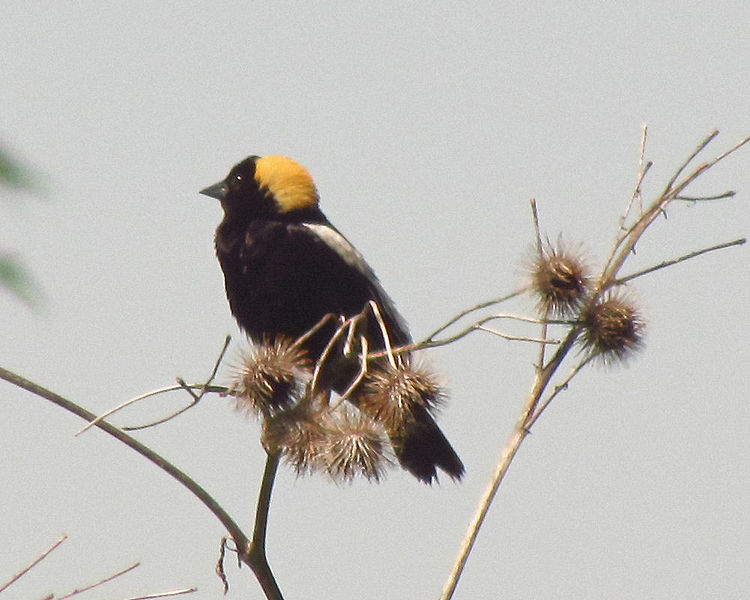
\includegraphics[width=1.2in]{Bobolink.jpg}
%\tiny {\sf (male)}
}
%\end{figure}

%\includegraphics[width=0.98\linewidth,height=.33\linewidth]{fig2_NLP.pdf}
\includegraphics[width=0.92\linewidth,height=.46\linewidth]{probDef_overall.png}
%\caption{Problem Definition: Zero-shot learning with textual description. Left: synopsis of textual descriptions for bird classes. Middle: images for ``seen classes''. Right: classifier hyperplanes in the feature space. The goal is to estimate a new classifier parameter given only a textual description}
\caption{ Top: Example Wikipedia article about the Painted Bunting, with an example image. Bottom: The proposed learning setting. For each category we are give one (or more) textual description (only a synopsis of a larger text is shown),  and a set of training images. Our goal is to be able to predict a classifier for a  category based only on the narrative (zero-shot learning). }
\label{F:prob_def}
\vspace{-14pt}
\end{figure*}
%Let us consider the problem of subordinate categorization of bird species as a case example. 
In this problem, When we learn from an expert about different species of birds, the teacher will not just give you sample images of each species and their class labels; the teacher will tell you about discriminative visual or non-visual features for each species, similarity and differences between species, hierarchal relations between species, and many other aspects. The same learning experience takes place when you read a book or a web page to learn about the different species of birds; For example, Fig.~\ref{F:prob_def} shows an example narrative about the {\sf Bobolink}. Typically, the narrative tells you about the bird's taxonomy, highlights discriminative features about that bird and discusses similarities and differences between species, as well as within-species variations (male vs. female). The narrative might eventually show very few example images, which are often selected wisely to illustrate certain visual aspects that might be hard to explain in the narrative.  This learning strategy using textual narrative and images makes the learning effective without a huge number of images  that a typical visual learning algorithm would need to learn the class boundaries. 
 
 





%Unnecessary details in images and text
 
%Although a narrative about a specific species can give very useful hints about what to look for to identify instances of that category, it also typically gives abundant of information about the species such as its habitat, diet, mating habits, etc. Such information is typically not useful for the task of the identification/recognition. In a sense, this information might be textual clutter for that task.  The same problem takes place in images, while one image can be very effective in highlighting an important feature for learning; typically images would have a lot of visual clutter that makes their uses in learning not effective. Many images of a given class might not provide discriminative features, and in fact can cause more confusion to a classifier. The point is a picture can worth a thousand words, but not always, and abundant of pictures might not be the most effective way for learning. Similarly one text paragraph can worth a thousand pictures for learning a concept, but not always, and abundant of text is not necessarily effective.  

%\begin{figure*}[t]
%
%!TEX root =  NLPVision_proposal.tex

%\begin{figure}

\parbox{5.5in}{
\tiny
{\sf
The Bobolink (Dolichonyx oryzivorus) is a small New World blackbird and the only member of genus Dolichonyx.

\vspace{2pt}
Description: Adults are 16-18 cm (6-8 in) long with short finch-like bills. They weigh about 1 oz. Adult males are mostly black, although they do display creamy napes, and white scapulars, lower backs and rumps. Adult females are mostly light brown, although their coloring includes black streaks on the back and flanks, and dark stripes on the head; their wings and tails are darker. The collective name for a group of bobolinks is a chain.

\vspace{2pt}
Distribution and movement: These birds migrate to Argentina, Bolivia and Paraguay. One bird was tracked flying 12,000 mi over the course of the year, and up to 1,100 mi in one day. They often migrate in flocks, feeding on cultivated grains and rice, which leads to them being considered a pest by farmers in some areas. Although Bobolinks migrate long distances, they have rarely been sighted in Europe-like many vagrants from the Americas, the overwhelming majority of records are from the British Isles. 
Each fall, Bobolinks gather in large numbers in South American rice fields, where they are inclined to eat grain. This has earned them the name "ricebird" in these parts. However, they are called something entirely different in Jamaica (Butterbirds) where they are collected as food, being that they are very fat as they pass through on migration.


\vspace{2pt}
Behavior:
Their breeding habitats are open grassy fields, especially hay fields, across North America. In high-quality habitats, males are often polygynous. Females lay 5 to 6 eggs in a cup-shaped nest, which is always situated on the ground and is usually well-hidden in dense vegetation. Both parents feed the young. 
Bobolinks forage on or near the ground, and mainly eat seeds, insects, cultivated grains and rice.
Males sing bright, bubbly songs in flight; these songs gave this species its common name.
}}
\parbox{1.4in}{
\centering
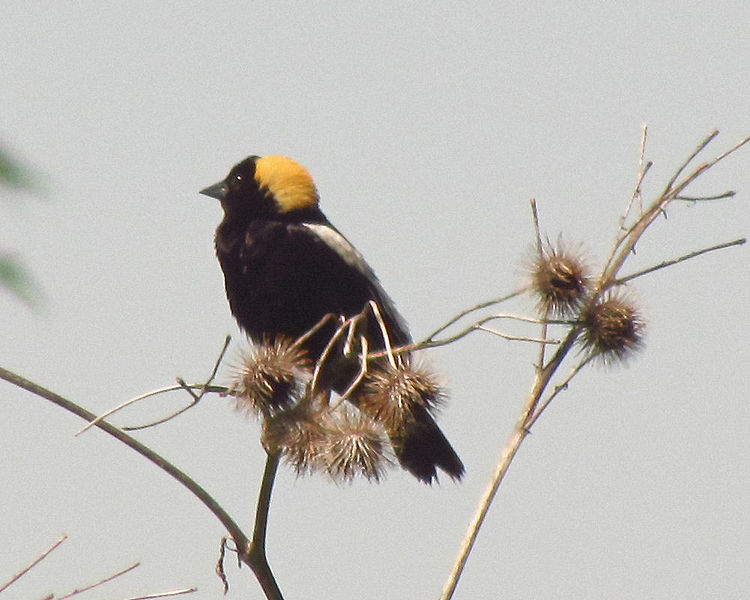
\includegraphics[width=1.2in]{Bobolink.jpg}
%\tiny {\sf (male)}
}
%\end{figure}


%\vspace{0.4cm}
%\includegraphics[width=0.99\linewidth,height=.27\linewidth]%{Text_vision_problemdef2.pdf}
%\label{F:prob_def}
%\vspace{-0.3cm}
%\caption{\footnotesize Top: Example Wikipedia article about the Painted Bunting, with an example image. Bottom: The proposed learning setting. For each category we are give one (or more) textual description (only a synopsis of  a larger text is shown),  and a set of training images. The first goal is to learn classifiers and detector for each bird species  jointly from the narrative and the images. A second goal  is to be able to predict a classifier and/or detector for a bird category only based only on the narrative (zero-shot learning). }
%\vspace{-15pt}
%\end{figure*}




%SM I changed slightly the above (I kept if need to get back to)
However, a narrative about a specific species does not contain only ``visually" relevant information, but also gives abundant information about the species's habitat, diet, mating habits that is not relevant for visual identification. In a sense, this information might be textual clutter for that task. The same problem takes place in images. While one image can be very effective in highlighting an important feature for learning, many images  might have a lot of visual clutter that makes their uses in learning not effective. %Many images of a given class might not provide discriminative features, and in fact can cause more confusion to a classifier. 
Thus, a picture can be worth a thousand words, but not always, and an abundant number of pictures might not be the most effective way for learning. Similarly, one text paragraph can be worth a thousand pictures for learning a concept, but not always, and large amounts of text might not necessarily be effective.





 

\textbf{Contributions.} The contribution of the paper is on exploring this new problem, which to the best of our knowledge, is firstly explored in the computer vision community in this work. We learn from an image corpus and a textual corpus, however not in the form of image-caption pairs, instead the only alignment between the corpora is at the level of the category. In particular, we address the problem of formulating a visual classifier prediction function ${\Phi (\cdot)}$, which predicts a  classifier of unseen visual class given its text description; see figure~\ref{F:prob_def}.  While a part of this work was  published in~\cite{Hoseini13}, we extend the work here to study more formulations to solve the problem in Sec.~\ref{formulation} (B,E). In addition, we also propose a kernel method to explicitly  predict a kernel classifier  in the form defined in the representer theorem~\cite{rth01}.  The kernelized prediction has an advantage that it opens the door for using any kind of side information about classes, as long as kernels can be used on the side information representation.  The side information can be in the form of textual, parse trees, grammar, visual representations, concepts in the ontologies (adopted in NLP domain), or any form. We focus here on unstructured text descriptions.\ignore{; see figure~\ref{fig:problem}} The image features also do not need to be in a vectorized format. The kernelized classifiers also facilitates combining different types of features through a multi-kernel learning (MKL) paradigm, where the fusion of different features can be effectively achieved.

\ignore{We propose and investigate two baseline formulations based on regression and domain adaptation. Then we propose a new constrained optimization formulation that combines a regression function and a knowledge transfer function with additional constraints to solve the problem.} 

Beyond the introduction and the related work sections, the paper is structured as follows: Sec~\ref{obvformulation} and ~\ref{sec_reganKT} details the problem definition and relation to regression and knowledge transfer models. Sec~\ref{formulation} shows different formulations of $\Phi(\cdot)$ that we studied to predict a linear visual classifier; see figure~\ref{F:prob_def}. Section~\ref{sec:app} developed extends our notion where  $\Phi(\cdot)$ predicts kernel classifier in the form defined by the representer theorem~\cite{rth01}. Sec~\ref{dskernel} presents our proposed distributional semantic kernel  between unstructured text description, which is applicable to  our kernel formulation and could be useful for other applications. Sec~\ref{experiments} presents our experiments  on Flower Dataset~\cite{Flower08} (102 classes) and Caltech-UCSD dataset~\cite{CU20010} (200 classes) for both the linear and the kernel classifier prediction.



%\section{Introduction NSF}
%\input{introNSFProposal}

\section{Related Work}
\label{relwork}
%!TEX root =  Write_a_classifier.tex

We focus our related work discussion on three related lines of research: ``zero/few-shot learning'', ``visual knowledge transfer'', and ``Language and Vision''.


%In general, knowledge transfer aims at enhancing recognition by exploiting shared knowledge between classes. This can come in different ways. Sharing knowledge can by achieved by enforcing a hierarchical structure on the classes, general to specific. Such hierarchy is used to impose constraints on the classifier parameters.  Such hierarchies can be exported from text domain, e.g., WordNet, or learned from visual features.  Our work can be seen in this context, where, we use learned visual classifiers and textual information to learn across-domain correlation that facilitates the prediction of visual classifiers for unseen classes. 

\textbf{Zero/Few-Shot Learning: }Similar to the setting of zero-shot learning, we use classes with training data (seen classes) to predict classifiers for classes with no training data (unseen classes).  Recent works on zero-shot learning of object categories focused on leveraging knowledge about common attributes and shared parts~\cite{Lampert09}.  Typically, attributes ~\cite{babak,Farhadi09}  are manually defined by humans and are used to transfer knowledge between seen and unseen classes.  In contrast, in our work we do not use any explicit attributes. The description of a new category is purely textual and the process is totally automatic without human annotation beyond the class labels.


Motivated by the practical need to learn visual classifiers of rare categories, researchers have explored approaches for learning from a single image (one-shot learning~\cite{Miller2000,fe2003bayesian,Fink04,BartU05}) or even from no images (zero-shot learning).
One way of recognizing object instances from previously unseen test categories
(the zero-shot learning problem) is by leveraging knowledge about common attributes and shared parts.
Typically an intermediate semantic layer is introduced to enable sharing knowledge between classes and facilitate describing knowledge about novel unseen classes, \eg~\cite{Palatucci09}.
 For instance, given adequately labeled training data, one can learn classifiers for the attributes occurring in the training object categories. These classifiers can then be used to recognize the same attributes in object instances from the novel test categories. Recognition can then proceed on the basis of these learned attributes~\cite{Lampert09, Farhadi09}. Such attribute-based ``knowledge transfer'' approaches use an intermediate visual attribute representation to enable describing unseen object categories. Typically attributes are manually defined by humans to describe shape, color, surface material, \eg, furry, striped, \etc  Therefore, an unseen category has to be specified in terms of the used vocabulary of attributes.  Rohrbach \etal~\cite{rohrbach10eccv} investigated extracting useful attributes from large text corpora. In~\cite{ParikhG11},  an approach was introduced for interactively defining a vocabulary of attributes that are both human understandable and visually discriminative. Huang \etal~\cite{Huang_2015_CVPR} relaxed the attribute independence assumption by modeling correlation between attributes to achieve better zero shot performance, as opposed to prior models. 
 In contrast, our work does not use any explicit attributes. The description of a new category is purely textual. 
 
 

\textbf{Visual Knowledge Transfer: }Our proposed work can be seen in the context of knowledge sharing and inductive transfer. 
In general, knowledge transfer aims at enhancing recognition by exploiting shared knowledge between classes. Most existing research focused on knowledge sharing within the visual domain only, \eg~\cite{griffin2008learning}; or exporting semantic knowledge at the level of category similarities and hierarchies, \eg~\cite{fergus2010semantic,Salakhutdinov11}.  We go beyond the state-of-the-art to explore cross-domain knowledge sharing and transfer. We explore how knowledge from the visual and textual domains can be used to learn across-domain correlation, which facilitates prediction of visual classifiers from textual description.  


%Another promising knowledge transfer direction is based on learning an intermediate layer of visual attributes that are shared among different classes. An object class is then defined as a combination of attributes using a class-attribute association matrix. For example~\cite{} uses web text mining to generate such association.    

%For the task of zero shot learning, Bart and Ullman \cite{BartU05} provided a set of similar object classes for a new class by finding nearest neighbors with similarity measure defined as the class confidence as output of classifiers for known object classes. Another group of works transfer knowledge of known classes by acquiring learned distance matrices \cite{Fink04} or by estimating object class priors \cite{Yu2010} or by defining functions over feature spaces \cite{Palatucci09}.


%Also the majority of zero-shot learning approaches focus on dataset with as a small number of categories (\eg animal dataset with 50 categories); instead we address the problem in the context of fine-grained recognition.


\textbf{Language and Vision:} The relation between linguistic semantic representations and visual recognition have been explored. For example in~\cite{deng2010does}, it was shown that there is a strong correlation between semantic similarity between classes, based on WordNet, and confusion between classes. Linguistic semantics in terms of nouns from WordNet \cite{wordNet95} have been used in collecting large-scale image datasets such as ImageNet\cite{imNet09} and Tiny Images~\cite{tinyimages}. It was also shown that hierarchies based on WordNet are useful in learning visual classifiers, \eg~\cite{Salakhutdinov11}.



%There have been some work on finding concepts and attributes for visual recognition through online text mining.  


One of the earliest work on learning from images and text corpora is the work of Barnard \etal~\cite{barnard2001clustering}, which showed that learning  a joint distribution of words and visual elements facilitates clustering the images in a semantic way, generating illustrative images from a caption, and generating annotations for novel images.
There has been an increasing recent interest in the intersection between computer vision and natural language processing with researches that focus on generating textual description of images and videos, \eg~\cite{farhadi2010every,kulkarni2011baby,yang2011corpus,krishnamoorthy2013generating}. This includes generating sentences about objects, actions, attributes, patial relation between objects, contextual information in the images, scene information, \etc
        ~In contrast, our work is different in two fundamental ways. In terms of the goal, we do not target generating textual description from images, instead we target  predicting classifiers from text, in a zero-shot setting. In terms of the learning setting, the textual descriptions that we use is at the level of the category  and do not come in the form of image-caption pairs, as in typical datasets used for text generation from images, \eg~\cite{ordonez2011im2text}. Recent impressive works has been proposed for image captioning (e.g., ~\cite{karpathy2014deep,vinyals2015show,xu2015show,mao2015deep}), which are based on the success of sequence to sequence training of neural nets 
%in  machine translation systems 
for translation 
(e.g.,~\cite{cho2014learning}).  In contrast, our work focus on a different  setting, which is  transforming an Encyclopedia text description to visual classifier.


There are several recent works that involved unannotated text\ignore{ \cite{NIPS13DeViSE,NIPS13CMT,Hoseini13}}.  In \cite{NIPS13DeViSE} and ~\cite{NIPS13CMT},  word  embedding language models (\eg ~\cite{wvecNIPs13}) was adopted to represent class names as vectors which requires training using a  big text-corpus. Their goal is to embed images into the language space then perform classification. There are several differences between these works and our method. First, one limitation of the adopted language model is that it produces only one vector per word, which produces problems when a word has multiple meanings.  Second, it can not represent a big text description of a class instead of a single or few words or others forms that could be ambiguous. Third,  our goal is different which is to map the text description to a classifier in the visual domain, \ie the apposite direction of their goal. Forth, these models do not support non-linear classification, supported by the kernelized version proposed in this work\ignore{, which is supported by our method}. We finally focus on fine-grained recognition, which is very  challenging\ignore{; see figure~\ref{fig:problem}}.  %Furthermore, focusing on the fine-grained settings makes it important. 



We can summarize the features of our proposed framework in contrast to prior work as follows: 1) Our framework explicitly predicts classifiers; 2) The predicted classifiers could be linear or  kernelized; 3) The approach requires the text description at the class level, not at the image level, hence, it needs only weak annotation. %4) While we focus on unstructured text description, we showed in one experiment that our approach could be used in attribute representation per class instead of text. %, allowing the use of continuous attributes and we do not require a confidence function for each attribute given the image and our models do not assume independence between attributes. 


%The rest of this paper is organized as follows. Section~\ref{obvformulation} presents the problem definition. Section~\ref{formulation} presents different methods for linear classifier prediction models from pure text description. Section~\ref{Knewapproach3_g2} presents a kernelized version of the final approach. Finally, section ~\ref{experiments} presents the experimental evaluation for the proposed formulations.  

%For example~\cite{} uses text sources like � to discover semantic relatedness among object categories which is shown to improve recognition. 

%%%


%In some other works on zero shot learning the concept of acquired knowledge has been moved from original space of visual features to a higher level space, understandable by humans which is called atribute space.   Attribute based representation of objects have gained an extensive amount of information in computer vision recently. As visual attributes can be learned in a generative framework featuring shared visual aspects of object classes, they can be used for describing objects that have not been seen before. This paradigm has been explored by Farhadi et al \cite{Farhadi09} by moving from object naming to object description. In this way an unseen object can be described by a set of visual attributes while the object is not nameable. In this case they state the problem of zero shot learning by finding nearest neighbors in the space of attributes. Lampert et al \cite{Lampert09} use attributes to manually relate object classes to a set of common attributes. Having this framework they are able to characterize unseen object classes while they have not seen any example of those classes during training. Rohrbach et al \cite{rohrbach10cvpr} acquire this framework and enhance it by moving from manually annotating object by attributes to automatically extracting useful attributes from large text corpora \cite{rohrbach10eccv,rohrbach11cvpr}

%Salakhutdinov et al\cite{Salakhutdinov11} capture the relationship between object classes by a hierarchical model and take advantage of this relationship to empower the classification task for the rare objects. They represent a tree structure to connect object classes to each other and share visual features between object classes that are similar based on this tree. This model can be used for the problem of zero shot learning by learning on top of similar object classes. 










\section{Problem Definition}
\label{obvformulation}
%!TEX root =  Write_a_classifier.tex


Fig~\ref{F:prob_def} illustrates the learning setting. 
The information in our problem comes from two different domains: the visual domain  and the textual domain, denoted by $\mathcal{V}$ and $\mathcal{T}$, respectively. Similar to traditional visual learning problems, we are given training data in the form $V=\{({x}_i , l_i)\}_{N}$, where $x_i$ is an image and $l_i \in \{1\cdots N_{sc}\}$ is its class label. We denote the number of classes available at training as $N_{sc}$, where $sc$ indicates ``seen classes''. As typically done in visual classification setting, we can learn $N_{sc}$ binary one-vs-all classifiers, one for each of these classes.  

Our goal is to be able to predict a classifier for a new category based only on the learned classes and a textual description(s) of that category. In order to achieve that, the learning process has to also include textual description of the seen classes (as shown in Fig ~\ref{F:prob_def} ). Depending on the domain we might find a few, a couple, or as little as one textual description to each class. We denote the textual training data for class $j$ by $\{t_i\in \mathcal{T} \}^j$. 
In this paper we assume we are dealing with the extreme case of having only one textual description available per class, which makes the problem even more challenging. For simplicity, the text description of class $j$ is denoted by $t_j$. However, the formulation we propose in this paper directly applies to the case of multiple textual descriptions per class.



In this paper, we cover predicting  visual classifier ${\Phi}(t_*)$ from an unseen text description $t_*$  in  linear form or RKHS kernalized form, defined as follows 


\subsection{Linear Classifier}
\label{sec_lin_pdef}
Let us consider a typical \ignore{binary }linear classifier in the feature space in the form
\[
    f_j(\mathbf{x}) = \mathbf{c}_j^\textsf{T} \cdot \mathbf{x}
\] 
where $\mathbf{x}$ (bold) is the visual feature vector of an image $x$ (not bold) amended with 1   and $\mathbf{c}_j \in \mathbb{R}^{d_v}$ is the linear classifier parameters for class $j$. Given a test image, its class is determined by
\begin{equation}
\small
l^* = \arg \max_j f_j(\mathbf{x})
\label{eq:mclass}
\end{equation}
  
 Similar to the visual domain, the raw textual descriptions have to go through a feature extraction process\ignore{, which will be described in Sec~\ref{experiments}}. Let us denote the linear extracted textual feature by 
$T=\{\mathbf{t}_j \in \mathbb{R}^{d_t}\}_{j=1\cdots N_{sc}}$, where $\mathbf{t}_j$ is the features of text description $t_j$ (not bold).  Given a textual description ${t}_*$  of a new unseen category $\mathcal{U}$  with linear feature vector representation $\mathbf{t}_*$, the problem can now be defined as predicting a one-vs-all linear classifier parameters ${\Phi}{(t_*)} = c(\mathbf{t}_*) \in \mathbb{R}^{d_v}$,  such that it can be directly used to classify any test image $\mathbf{x}$ as 
\begin{eqnarray}
      c(\mathbf{t}_*)^\textsf{T} \cdot \mathbf{x} >  0 & \text{if} \;  \mathbf{x} \; \text{belongs to} \;\mathcal{U} \nonumber \\
      c(\mathbf{t}_*)^\textsf{T} \cdot \mathbf{x} <  0 &  \text{otherwise} \label{E:PredictedClass}
\end{eqnarray}

%$c(\mathbf{t}_*)$ is detailed in Sec~\ref{formulation}. 

\subsection{Kernel Classifier}
\label{sec_kernel_pdef}
For kernel classifiers, we assume that each of the domains is equipped with a kernel function corresponding to a \textit{reproducing kernel Hilbert space} (RKHS). Let us denote the kernel for $\mathcal{V}$ by $k(\cdot,\cdot)$, and the kernel for $\mathcal{T}$ by $g(\cdot,\cdot)$. %At the zero-shot time,  \ignore{information  is presented as \small$D_{test} = \{ \mathcal{S}_x^*= \{ {x}^*_j \}_{N'}, \mathcal{S}_e^* = \{ y^*_j, {e}_{y^*_j} \}_{N_{us}} \}$\normalsize, where  \small${x}^*_j \in \mathcal{X}$\normalsize, \small$y^*_j \in {Y}_{us}$\normalsize (test/unseen labels), \small$\mathcal{S}_x^*$\normalsize is  a set of \small$N'\,$\normalsize test points in \small$\mathcal{X}$\normalsize domain, and privileged information \small$\mathcal{S}_e^*\,$\normalsize is available for the unseen classes and \small${e}_{y^*_j} \in \mathcal{E}$\normalsize.}only the text description    ${t}_{*}$ is available for each novel unseen class.
\ignore{Since, we are studying explicit kernel-classifier prediction from privileged information, we first present an overview on multi-class classification on kernel space.  One} 
\normalsize 

%The  common approach for multi-class classification is to learn a classifier for each class against the remaining classes (i.e. one-vs-all). 
According to the generalized representer theorem~\cite{rth01},  a minimizer of a regularized empirical risk function over an RKHS could be represented as a linear combination of kernels, evaluated on the training set. Adopting the representer theorem on classification risk function, we define a kernel-classifier of a visual class $j$ as follows


\begin{equation}
\small
\begin{split}
f_j({x})=&   \sum_{i=1}^{N} \beta_j^i k({x}, {x}_i) + b  = \sum_{i=1}^{N} \beta_j^i \varphi({x_i})^\textsf{T} \varphi( {x}) + b \\
f_j({x})=&  {\boldsymbol{\beta}_j}^\textsf{T} \cdot  \textbf{k}({x}) =  \mathbf{c}_j^\textsf{T} \cdot [\varphi(x); 1] , \mathbf{c}_j =  [\sum_{i=1}^{N} \beta_j^i \varphi({x_i}); b]\\
%&, 
\end{split}
\label{eq_fkernel}
\end{equation}
where ${x} \in \mathcal{V}$ is the test image, ${x}_i$ is the $i^{th}$ image in the training data $V$,  $\textbf{k}({x})= [k({x}, {x}_1), \cdots, k({x}, {x}_N), 1]^\textsf{T},$  $\boldsymbol{\beta}_j = [\beta_j^1 \cdots \beta_j^N, b]^\textsf{T} $. Having learned $f_j({x}^*)$ for each class $j$ (for example using SVM classifier), the class label of the test image ${x}$ can be predicted by  Eq.~\ref{eq:mclass}, similar to the linear case. Eq.~\ref{eq_fkernel} also shows how $\boldsymbol{\beta}_j$ is related to $\mathbf{c}_j$ in the linear classifier, where $k(x, x')= \varphi(x)^\mathsf{T} \cdot \varphi(x')$ and $\varphi(\cdot)$ is a feature map  that does not have to be defined given $k(\cdot, \cdot)$ on $\cal{V}$. Hence, our goal in the kernel classifier prediction  is to predict $\boldsymbol{\beta}(t_*)$ instead of $\mathbf{c}(t_*)$ since it is sufficient to define  ${f}_{t_*}(x)$ for a text description $t_*$ of an unseen class given $\mathbf{k}(x)$

%\small
%\begin{equation}
%  l^* = \arg \max_k f_k(\mathbf{x}^*)
%  \label{eq:mclass}
%\end{equation}
%\normalsize

\ignore{Under our setting, i}It is clear that $f_j({x})$ could be learned for  all classes with training data $j \in  {1} \cdots {N_{sc}}$, since there are examples for the seen classes; we denote the kernel-classifier parameters of the seen classes as $\mathcal{B}_{sc} =  \{  \boldsymbol{\beta}_j \}_{N_{sc}}, \forall j$. However, it is not obvious how to predict $f_{{t}_*}({x})$ for an unseen class given its text description ${t}_*$. Similar to the linear classifier prediction, our main notion is to use the text description ${t}_{*}$, associated with unseen class, and the training data to directly predict the unseen kernel-classifier parameters. In other words, the kernel classifier parameters of the unseen class is a function of  its text description ${t}_*$ , the image training data $V$ and the text training data $\{t_j\}, j\in 1 \cdots N_{sc}$; \ie \small
\[   f_{{t}_*}({x}) = \boldsymbol{\beta}({t}_*)^\textsf{T} \cdot \textbf{k}({x}), \] \normalsize
 $ f_{{t}_*}({x})$ could be used to classify new points that	 belong to an  unseen class as follows: 1) one-vs-all setting  $f_{{t}_*}({x})  \gtrless  0$  \ignore{if ${x}^*\,$  belongs to unseen category $z^*$, $\boldsymbol{\beta}(\mathbf{t}_*),)^\textsf{T} \cdot \textbf{k}(x^*)< 0$  otherwise}; or 2) in a Multi-class prediction as in Eq~\ref{eq:mclass}. ${\Phi}(t_*)$ in this case is $\boldsymbol{\beta}({t}_{*})$. In contrast to linear classifier prediction, there is no need to explicitly represent an image $x$ or a text description $t$ by features, which are denoted by the bold symbols in the previous section. Rather, only the  $k(\cdot,\cdot)$  and $g(\cdot,\cdot)$ needs to be defined which is general. 



\section{Relation to Regression and Knowledge Transfer Models}
\label{sec_reganKT}
We introduce two possible frameworks for this problem and discuss potential limitations for them. In this background section,  we focus on predicting linear classifiers for simplicity, which motivates the the evaluated linear classifier formulations that follow in Sec~\ref{formulation}. 

\subsection{Regression Models}
A straightforward way to solve this problem is to pose it as a regression problem where the goal is to use the textual data and the learned classifiers, $\{(\mathbf{t}_j,\mathbf{c}_j) \}_{j=1\cdots N_{sc}}$ to learn a regression function from the textual feature domain to the visual classifier domain, \ie, a function $c(\cdot) : \mathbb{R}^{d_t} \rightarrow \mathbb{R}^{d_v} $.  The question is which regression model would be suitable for this problem? and would posing the problem this way give reasonable results?

A typical regression model, such as ridge regression~\cite{ridgeReg70} or Gaussian Process (GP) Regression~\cite{Rasmussen:2005}, learns the regressor to each dimension of the output domain (the parameters of a linear classifier) separately, \ie,  a set of functions $c^i(\cdot) : \mathbb{R}^{d_t} \rightarrow \mathbb{R} $. Clearly this will not capture the correlation between the visual classifier dimensions. Instead, a structured prediction regressor would be more suitable since it would learn the correlation between the input and output domain. However, even a structured prediction model, will only learn the correlation between the textual and visual domain through the information available in the input-output pairs  $(\mathbf{t}_j,\mathbf{c}_j)$.  Here the visual domain information is encapsulated in the pre-learned classifiers and prediction does not have access to the original data in the visual domain. Instead we need to directly learn the correlation between the visual and textual domain and use that for prediction.

Another fundamental problem  that a regressor would face, is the sparsity of the data; the data points are the textual description-classifier pairs, and typically the number of classes can be very small compared to the dimension of the classifier space (\ie $N_{sc} \ll d_v$). In a setting like that, any regression model is bound to suffer from an under fitting problem. This can be best explained in terms of GP regression, where the predictive variance increases in the regions of the input space where there are no data points. This will result in  poor prediction of classifiers at these regions. 

\subsection{Knowledge Transfer Models}
An alternative formulation is to pose the problem as domain adaptation from the textual to the visual domain. In the computer vision context, domain adaptation work has focused on transferring categories learned from a source domain,  with a given distribution of images, to a target domain with different distribution, \eg, images or videos from different sources~\cite{yang07,saenko10,da11,duan12}. 
What we need is an approach that learns the correlation between the textual domain features and the visual domain features, and uses that correlation to predict new visual classifier given textual features. 

In particular, in~\cite{da11} an approach for learning cross domain transformation was introduced. In that work a regularized asymmetric transformation between points in two domains were learned. The approach was applied to transfer learned categories between different data distributions, both in the visual domain. A particular attractive characteristic of~\cite{da11}, over other domain adaptation models, is that the source and target domains do not have to share the same feature spaces or the same dimensionality. 

While a totally different setting is studied in ~\cite{da11}, it inspired us to formulate the zero-shot learning problem as a domain transfer problem. This can be achieved by learning a linear transfer function $\mathbf{W}$ between $\mathcal{T}$ and $\mathcal{V}$.  The transformation matrix $\mathbf{W}$ can be learned  by optimizing, with a suitable regularizer, over constraints of the form $\mathbf{t}^\textsf{T}\mathbf{W}\mathbf{x} \geq l $ if $\mathbf{t} \in \mathcal{T}$  and $\mathbf{x}\in \mathcal{V}$  belong to the same class, and $\mathbf{t}^\textsf{T}\mathbf{W}\mathbf{x} \leq u $  otherwise. Here $l$ and $u$ are model parameters. This transfer function acts as a compatibility function between the textual features and visual features, which gives high values if they are from the same class and a low value if they are from different classes. 

%It is not hard to see that this transfer function, learned on seen classes can act as a classifier for unseen classes. Given a textual feature $\mathbf{t}^*$ for an unseen class and a test image $\mathbf{x}$ a classification decision can be obtained by $\mathbf{t}_*^\textsf{T}\mathbf{W}\mathbf{x} \gtrless b$ where $b$ is a decision boundary which can be set to $(l+u)/2$. It is also not hard to see that our desired predicted classifier in Eq~\ref{E:PredictedClass} can be obtained as $c(\mathbf{t}_*) = \mathbf{t}_*^\textsf{T}\mathbf{W} $. 

It is not hard to see that this transfer function can act as a classifier. Given a textual feature $\mathbf{t}^*$ and a test image, represented by $\mathbf{x}$, a classification decision can be obtained by $\mathbf{t}_*^\textsf{T}\mathbf{W}\mathbf{x} \gtrless b$ where $b$ is a decision boundary which can be set to $(l+u)/2$. Hence, our desired predicted classifier in Eq~\ref{E:PredictedClass} can be obtained as $c(\mathbf{t}_*) = \mathbf{t}_*^\textsf{T}\mathbf{W} $ (note that the features vectors are amended with ones).  However, since learning  $\mathbf{W}$ was done over seen classes only, it is not clear how the predicted classifier $c(\mathbf{t}_*)$ will behave for unseen classes. There is no guarantee that such a classifier will put all the seen data on one side and the new unseen class on the other side of that hyperplane. 





%\begin{eqnarray}
%\mathbf{t}^\textsf{T}\mathbf{W}\mathbf{x} \geq l & \text{if} \mathbf{t} \in \mathcal{T}  \text{and} \mathbf{x}\in \mathcal{V}  \text{belong to the same class} \\ 
%\mathbf{t}^\textsf{T}\mathbf{W}\mathbf{x} \leq u & \text{otherwise}.
%\end{eqnarray}  


%



%\begin{figure}[h!]
%  \label{fig:mdlOfrgMdl}
%  \centering
%    \includegraphics[width=0.4\textwidth]{mdlOfrgMdl.jpg}
%   \caption{Model of Regression Models Lack of Data underfitting, The gray level indicate the uncertainty region, black line is the prediction, the blue line is the ground truth model}
%\end{figure}




\section{Formulations for Predicting a linear   classifier form of ${\Phi (t_*)}$}
\label{formulation}
%!TEX root =  Write_a_classifier.tex
The proposed formulations in this section aims at predicting a linear hyperplane parameter $\mathbf{c}$ of a one-vs-all classifier for a new unseen class given a textual description, encoded as a feature vector $\mathbf{t_*}$ and the knowledge learned at the training phase from seen classes\footnote{The notations follow from Subsection~\ref{sec_lin_pdef}}. We start by  defining the learning components that were used by the formulations described in this section:

\begin{description}
\item [Classifiers:]$\,\,\,\,\,\,\,\,$ 

a set of linear one-vs-all classifiers $\{\mathbf{c}_j\}$ are learned, one for each seen class.
\item [Probabilistic Regressor:] $\,\,\,\,\,\,\,\,\,\,\,\,$

Given $\{(\mathbf{t}_j,\mathbf{c}_j)\}$ a regressor is learned that can be used to give a prior estimate for $p_{reg}(\mathbf{c} | \mathbf{t})$ (Details in Sec~\ref{S:Reg}).
\item [Domain Transfer:]$\,\,\,\,\,\,\,\,\,\,\,\,$ 

Given $T$ and $V$ a domain transfer function, encoded in the matrix $\mathbf{W}$ is learned, which captures the correlation between the textual and visual domains (Details in Sec~\ref{S:DA}).
\end{description} 
  
  
  
Each of the following subsections show a different approach to predict a linear classifier from $t_*$ as $\Phi(t_*) = \mathbf{c}(\textbf{t}_*)$; see Sec~\ref{sec_lin_pdef}. The final approach (E) combines  regression, domain transfer, and additional constraints, which achieves the best performance. We compare between these alternative formulations in our experiments. Hyper-parameter selection is detailed in the supplementary materials for all the approaches. % regression (A), constrained regression (B), domain transfer (C), (D) constrained regression and domain transfer,  and (E)  constrained domain transfer. Our best final formulation (E) combines the regression, domain transfer function, and additional constraints to achieve better performance.

\begin{figure*}[t]
\centering
\includegraphics[width=1.0\linewidth,height=.38\linewidth]{fig_NLP4.pdf}
\vspace{-10pt}
\caption{Illustration of the Proposed Linear Prediction Framework (Constrained Regression and Domain Transfer) for the task Zero-shot learning from textual description (Linear Formulation (E))}
\label{F:prob_sol}
\vspace{-12pt}
\end{figure*}

\subsection{Probabilistic Regressor}
\label{S:Reg}
There are different regressors that can be used, however we need a regressor that provide a probabilistic estimate $p_{reg}(\mathbf{c} | \mathbf(t))$. For the reasons explained in Sec~\ref{obvformulation}, we also need a structure prediction approach that is able to predict all the dimensions of the classifiers together. For these reasons, we use the Twin Gaussian Process (TGP)~\cite{Bo:2010}. 
TGP encodes the relations between both the inputs and structured outputs using Gaussian Process priors. This is achieved by minimizing the Kullback-Leibler divergence between the marginal GP of the outputs (i.e. classifiers in our case) and observations (i.e. textual features). The estimated regressor output ($\tilde{c}(\mathbf{t}_*)$) in TGP is given by the solution of the following non-linear optimization problem~\cite{Bo:2010} \footnote{notice we are using $\mathbf{\tilde{c}}$ to denote the output of the regressor, while using $\mathbf{\hat{c}}$ to denote the output of the final optimization problem in Eq~\ref{eq:form}}.
\begin{equation}                                               
\centering
\begin{split}
{\Phi (t_*)} = \tilde{c}(\mathbf{t}_*) = & \underset{\mathbf{c}}{\operatorname{argmin}}[  K_C(\mathbf{c},\mathbf{c})  -2 k_c(\mathbf{c})^\textsf{T} \mathbf{u} - \eta  \log ( \\ & K_C(\mathbf{c},\mathbf{c} -k_c(\mathbf{c})^\textsf{T} (\mathbf{K}_C+ \lambda_c \mathbf{I})^{-1} k_c(c) ) ]
\end{split}
\label{eq:tgp}
\end{equation}
where $\mathbf{u} = (\mathbf{K}_\textsf{T} + \lambda_t  \mathbf{I})^{-1} k_t(\mathbf{t}_*)$, $\eta  = K_T(\mathbf{t}_*,\mathbf{t}_*) -k(\mathbf{t}_*)^\textsf{T}  \mathbf{u} $,  $K_T(\mathbf{t}_l,\mathbf{t}_m) $ and $K_C(\mathbf{c}_l,\mathbf{c}_m)$ are Gaussian kernel for input feature $\mathbf{t}$ and output vector $\mathbf{c}$.  $k_c(\mathbf{c}) = [K_C(\mathbf{c},\mathbf{c}_1), \cdots, K_C($ $\mathbf{c},\mathbf{c}_{N_{sc}})]^\textsf{T}$. $k_t(\mathbf{t}_*) = [K_T(\mathbf{t}_*,\mathbf{t}_1), \cdots, K_T(\mathbf{t}_*,\mathbf{t}_{N_{sc})}]^\textsf{T}$.  $\lambda_t$ and $\lambda_c$ are regularization parameters to avoid overfitting. This optimization problem can be solved using a second order, BFGS quasi-Newton optimizer with cubic polynomial line search for optimal step size selection~\cite{Bo:2010}. In this case the classifier dimension are predicted jointly. In this case $p_{reg}(\mathbf{c}|\mathbf{t}_*)$ is defined as a normal distribution.
\begin{equation}
\label{eq:ptgp}
p_{reg}(\mathbf{c}|\mathbf{t}_*) =  \mathcal{N} (\mu_c = \tilde{c}(\mathbf{t}_*),\Sigma_c = \mathbf{I})
\end{equation}
The reason that $\Sigma_c = \mathbf{I}$ is that TGP does not provide predictive variance, unlike Gaussian Process Regression. However, it has the advantage of handling the dependency between the dimensions of the classifiers $\mathbf{c}$ given the textual features $\mathbf{t}$. 
 
\subsection{Constrained Probabilistic Regressor}
\label{S:Reg_con}
We also investigated formulations that use regression to predict an initial hyperplane  $\tilde{c}(\mathbf{t}_*)$ as described in section ~\ref{S:Reg}, which is then optimized to put all seen data in one side, \ie
\begin{equation*}
\begin{split}
 {\Phi (t_*)} = \small \hat{c}(\mathbf{t}_*) =   \underset{\mathbf{c},\zeta_i}{\operatorname{argmin }}[  \mathbf{c}^\textsf{T} \mathbf{c}  + \alpha \, \psi( \mathbf{c},\tilde{c}(\mathbf{t}_*)) + C   \sum_{i=1}^N{\zeta_i} ] \\ \; s.t.:  -\mathbf{c}^\textsf{T} {\mathbf{x}}_{i}  \geq \zeta_i , \; \zeta_i \geq 0 , i=1,\cdots,N 
\end{split}
\end{equation*}

where $\psi(\cdot,\cdot)$ is a similarity function between hyperplanes, \eg a dot product used in this work,  $\alpha$ is its constant weight, and $C$ is the weight to the soft constraints of existing images as negative examples (inspired by linear SVM formulation)\ignore{, or other functions incorporating the predictive variance}. We call this class of methods {\em constrained GPR/TGP}, since $\tilde{c}(\mathbf{t}_*)$ is initially predicted through GPR or TGP. 
 


\subsection{Domain Transfer (DT)}
\label{S:DA}
To learn the domain transfer function $\mathbf{W}$ we adapted the approach in~\cite{da11} as follows. Let $\mathbf{T}$ be the textual feature data matrix and $\mathbf{X}$ be the visual feature data matrix where each feature vector is amended with a 1. Notice that amending the feature vectors with a 1 is essential in our formulation since we need $\mathbf{t}^\textsf{T} \mathbf{W}$ to act as a classifier. We need to solve the following optimization problem 
\begin{equation}
  \min_{\mathbf{W}}  r(\mathbf{W}) + \lambda \sum_i c_i(\mathbf{T} \mathbf{W} \mathbf{X}^\textsf{T})
  \label{Eq:DA1}
\end{equation}
%where $c_i$'s are loss functions over the constraints and $r(\cdot)$ is a matrix regularizer.  It was shown in~\cite{da11}, under condition on the regularizer, that the optimal $\mathbf{W}$ in Eq~\ref{Eq:DA1} can be computed using inner products between data points in each of the domains separately, which results in a kernalized non-linear transfer function; hence its complexity does not depend on the dimensionality of either of the domains. The optimal solution of~\ref{Eq:DA1} is in the form
where $c_i$'s are loss functions over the constraints and $r(\cdot)$ is a matrix regularizer.  It was shown in~\cite{da11}, under condition on the regularizer, that the optimal $\mathbf{W}$  is in the form of 
 $ \mathbf{W}^* = \mathbf{T} \mathbf{K}_{T}^{-\frac{1}{2}} \mathbf{L}^*  \mathbf{K}_{X}^{-\frac{1}{2}} \mathbf{X}^\textsf{T}$, where  $\mathbf{K}_{T}  = \mathbf{T} \mathbf{T}^\textsf{T}$,  $\mathbf{K}_{X}  = \mathbf{X} \mathbf{X}^\textsf{T}$.   $\mathbf{L}^*$ is computed by minimizing the following minimization problem
\begin{equation}
 \underset{\mathbf{L}}{\operatorname{min       }}[   r(\mathbf{L})+ \lambda \sum_p c_p(\mathbf{K}_{T}^{\frac{1}{2}} \mathbf{L} \mathbf{K}_{X}^\frac{1}{2}  ) ],
\end{equation}
where $c_p(\mathbf{K}_{T}^{\frac{1}{2}} \mathbf{L} \mathbf{K}_{X}^\frac{1}{2}  ) = (max(0, (l-e_i \mathbf{K}_{T}^{\frac{1}{2}} \mathbf{L} \mathbf{K}_{X}^\frac{1}{2} e_j) ))^2$ for same class pairs of index $i$,$j$, or $ =(max(0, (e_i \mathbf{K}_{T}^{\frac{1}{2}} \mathbf{L} \mathbf{K}_{X}^\frac{1}{2} e_j -u) ))^ 2$ otherwise, where $e_k$ is a one-hot vector of zeros except a one at the $k^{th}$ element, and $u>l$ (note any appropriate $l$, $u$ could work. In our case, we used $l =2$, $u=-2$ ). We used a Frobenius norm regularizer.  This energy is minimized using a second order BFGS quasi-Newton optimizer. Once $L$ is computed $\textbf{W}^*$ is computed using the transformation above. Finally ${\Phi (t_*)}  = c(\mathbf{t}_*) = \mathbf{t}_*^\textsf{T}\mathbf{W}$, simplifying  $\textbf{W}^*$ as $\textbf{W}$.  




\subsection{Constrained-DT}
We also investigated constrained-DT formulations that learns a transfer matrix $\mathbf{W}$ and  enforce $\mathbf{t}_j^\textsf{T}\mathbf{W}$ to be close to the classifiers learned on seen data, $\{\mathbf{c}_j \}$ ,\ie
\[\small \min_{\mathbf{W}}  r(\mathbf{W}) + \lambda_1 \sum_i c_i(\mathbf{T} \mathbf{W} \mathbf{X}^\textsf{T}) +\lambda_2 \sum_k{(\mathbf{c}_j - \mathbf{t}^\textsf{T}_j \mathbf{W})^T (\mathbf{c}_j - \mathbf{t}^\textsf{T}_j \mathbf{W})}
\]
A classifier can be then obtained by ${\Phi (t_*)}  =c(\mathbf{t}_*)= \mathbf{t}_*^\textsf{T}\mathbf{W}$.
%A classifier can be obtained by optimizing an objective similar to Eq~\ref{Eq:Opt1} without the regression to obtain ${\Phi (t_*)}  = c(\mathbf{t}_*)$

\begin{comment}

\begin{equation}
\small
\begin{split}
 {\Phi (t_*)} = \small \hat{c}(\mathbf{t}_*) =   \underset{\mathbf{c},\zeta_i}{\operatorname{argmin }}[    \mathbf{c}^\textsf{T} \mathbf{c} - \alpha {\mathbf{t}_*}^\textsf{T} \mathbf{W} \mathbf{c}  - \gamma  
 \ln p_{reg}(\mathbf{c}|\mathbf{t}_*)
  \\ +\gamma   \sum_{i=1}^N{\zeta_i} ]\, ; s.t.:  -\mathbf{c}^\textsf{T} {\mathbf{x}}_{i}  \geq \zeta_i , \; \zeta_i \geq 0 , \; {\mathbf{t}_*}^\textsf{T} \mathbf{W} \mathbf{c} \geq l 
 \label{Eq:Opt1}
 \end{split}
 \end{equation}
The first term is a regularizer over the classifier $\mathbf{c}$.  The second term enforces that the predicted classifier has high correlation with $\mathbf{t}_*^\textsf{T} \mathbf{W}$. The third term favors a classifier that aligns with the prediction of the regressor $\tilde{c}(\mathbf{t}_*)$. The constraints $\mathbf{c}^\textsf{T} {\mathbf{x}}_{i} \geq \zeta_i $  enforce that all  seen data instances are at the negative side of the predicted hyperplane with some missclassification allowed through the  slack variables $ \zeta_i$. The constraint $ {\mathbf{t}_*}^\textsf{T} \mathbf{W} \mathbf{c} \geq l$ enforces that the correlation between the predicted classifier and ${\mathbf{t}_*}^\textsf{T} \mathbf{W}$ is no less than $l$, \ie a minimum correlation between the text and visual features. 
Given $\mathbf{W}$, and the form of the probability estimate $ p_{reg}(\mathbf{c}|\mathbf{t}_*)$, the optimization reduces to a quadratic program on $\mathbf{c}$ with linear constraints.
\end{comment}

\subsection{Constrained  Regression and Domain Transfer for classifier prediction}
 Fig~\ref{F:prob_sol} illustrates our final  framework which combines regression (formulation A (using TGP)) and domain transfer (formulation C) with additional constraints. This formulation combines the three learning components described in the beginning of this section. 
%At the training phase three components are learned:
%\begin{description}
%\item [Classifiers:] a set of one-vs-all classifiers $\{\mathbf{c}_k\}$ are learned, one for each seen class.
%\item [Probabilistic Regressor:] Given $\{(\mathbf{t}_k,\mathbf{c}_k)\}$ a regressor is learned that can be used to give a prior estimate for $p_{reg}(\mathbf{c} | \mathbf{t})$ (Details in Sec~\ref{S:Reg}).
%\item [Domain Transfer Function:] Given $T$ and $V$ a domain transfer function, encoded in the matrix $\mathbf{W}$ is learned, which captures the correlation between the textual and visual domains (Details in Sec~\ref{S:DA}).
%\end{description} 
Each of these components contains partial knowledge about the problem. The question is how to combine such knowledge to predict a new classifier given a textual description. The new classifier has to be consistent with the seen classes. 
The new classifier has to put all the seen instances at one side of the hyperplane, and has to be consistent with the learned domain transfer function. This leads to the following constrained  optimization problem 
\begin{equation}
\begin{split}
 {\Phi (t_*)} = \hat{c}(\mathbf{t}_*) =  &   \underset{\mathbf{c},\zeta_i}{\operatorname{argmin }}\big[    \mathbf{c}^\textsf{T} \mathbf{c} - \alpha {\mathbf{t}_*}^\textsf{T} \mathbf{W} \mathbf{c}  - \gamma  \ln( p_{reg}(\mathbf{c}|\mathbf{t}_*))  \\
& + C   \sum{\zeta_i} \big]\\
&s.t.:  -(\mathbf{c}^\textsf{T} {\mathbf{x}}_{i} ) \geq \zeta_i ,  \,\, \zeta_i \geq 0 ,\; \; i = 1 \cdots N \\
&	   \,\, {\mathbf{t}_*}^\textsf{T} \mathbf{W} \mathbf{c} \geq l     \\
& \alpha , \gamma, C, l \,  \text{: hyperparameters}\\ 
\end{split}
\label{eq:form}
\end{equation}
The first term is a regularizer over the classifier $\mathbf{c}$.  The second term enforces that the predicted classifier has high correlation with $\mathbf{t}_*^\textsf{T} \mathbf{W}$; $\mathbf{W}$ is learnt by Eq~\ref{Eq:DA1}. The third term favors a classifier that has high probability given the prediction of the regressor. The constraints $ -\mathbf{c}^\textsf{T} {\mathbf{x}}_{i} \geq \zeta_i $  enforce all the seen data instances to be at the negative side of the predicted classifier hyperplane with some missclassification allowed through the  slack variables $ \zeta_i$. The constraint $ {\mathbf{t}_*}^\textsf{T} \mathbf{W} \mathbf{c} \geq l$ enforces that the correlation between the predicted classifier and ${\mathbf{t}_*}^\textsf{T} \mathbf{W}$ is no less than $l$, this is to enforce a minimum correlation between the text and visual features. 


%>>> add ones to the vectors. when learning W


%The optimization problem above is a quadratic program on $\mathbf{c}$ with linear constraints. We tried different quadratic solvers, however CPLEX IBM solver \footnote{http://www-01.ibm.com/software/integration/optimization/cplex-optimizer} gives best performance in speed and optimization.


%%%%

\textbf{Solving for $\hat{c}$ as a quadratic program: }
According to  the definition of $p_{reg}(\mathbf{c}|\mathbf{t}_*)$ for  TGP,  $\ln p(\mathbf{c}|\mathbf{t}_*)$ is a quadratic term in $c$ in the form  
\begin{equation}
\begin{split}
-\ln p(\mathbf{c}|\mathbf{t}_*) \propto ( \mathbf{c} - \tilde{c}(\mathbf{t}_*))^\textsf{T} (\mathbf{c} - \tilde{c}(\mathbf{t}_*)) \\= \mathbf{c}^\textsf{T} \mathbf{c} -2 \mathbf{c}^\textsf{T} \tilde{c}(\mathbf{t}_*) +  \tilde{c}(\mathbf{t}_*)^\textsf{T} \tilde{c}(\mathbf{t}_*) 
\end{split}
\label{eq:lnptgp}
\end{equation}
We reduce $-\ln p(\mathbf{c}|\mathbf{t}_*)$ to $-2 \mathbf{c}^\textsf{T} \tilde{c}(\mathbf{t}_*))$, since 1) $\tilde{c}(\mathbf{t}_*)^\textsf{T} \tilde{c}(\mathbf{t}_*)$ is a constant (\ie does not affect the optimization), 2) $\mathbf{c}^\textsf{T} \mathbf{c}$ is already included as regularizer in equation ~\ref{eq:form}.  In our setting, the dot product  is a better similarity measure between two hyperplanes. Hence,  $-2 \mathbf{c}^\textsf{T} \tilde{c}(\mathbf{t}_*)$ is minimized.
Given $-\ln p(\mathbf{c}|\mathbf{t}_*)$ from the TGP and  $\mathbf{W}$, Eq~\ref{eq:form} reduces to a quadratic program on $\mathbf{c}$ with linear constraints. We tried different quadratic solvers, however the IBM CPLEX solver \footnote{http://www-01.ibm.com/software/integration/optimization/cplex-optimizer} gives the best performance in speed and optimization for our problem.


%\noindent{\bf Formulations:}
%We investigated several formulations for predicting classifier parameters $c(\mathbf{t}_*)$ for a new class with textual description $\mathbf{t}_*$, in the form of a linear one-vs-all classifier, \ie,
%$c(\mathbf{t}_*)^\textsf{T} \cdot \mathbf{x} >  0  \; \text{if} \;  \mathbf{x} \; \text{belongs to} \;\mathcal{C} $ and $c(\mathbf{t}_*)^\textsf{T} \cdot \mathbf{x} <  0   \;\; \text{otherwise}$.  Recall that the features are amended with 1 such that $c(\mathbf{t}_*)$ is hyperplane paramterization. Table~\ref{T:AUC} shows results of different formulations, which will be details next.
%\begin{eqnarray}
%      c(\mathbf{t}_*)^\textsf{T} \cdot \mathbf{x} >  0 & \text{if} \;  \mathbf{x} \; \text{belongs to} \;\mathcal{C} \nonumber \\
%      c(\mathbf{t}_*)^\textsf{T} \cdot \mathbf{x} <  0 &  \text{otherwise} \label{E:PredictedClass}
%\end{eqnarray}

%\medskip
%\noindent{\em Regression Models:} Given classifiers learned on seen classes, with hyperplanes  $\{\mathbf{c}_k\}$, and the corresponding textual features $\{\mathbf{t}_k\}$, we can learn a regression function $c(\cdot) : \mathbb{R}^{d_t} \rightarrow \mathbb{R}^{d_v} $ from $ \mathcal{T}$ to $ \mathcal{V}$. We investigated Gaussian Process Regression (GPR)~\cite{Rasmussen:2005} and structured regression using the Twin Gaussian Processes (TGP)~\cite{Bo:2010}.  However such regression model will only learn the correlation between the textual and visual domain through the information available in its input-output pairs, \ie  $(\mathbf{t}_k,\mathbf{c}_k)$.  Here the visual domain information is encapsulated in the pre-learned classifiers, and prediction does not have access to the original data in the visual domain. Another problem, is the sparsity of the data; the number of training classes is typically much less than the dimension of the visual and textual feature spaces. 
%We also investigated formulations that use regression to predict an initial hyperplane  $\tilde{c}(\mathbf{t}_*)$, which is then optimized to put all seen data in one side, \ie
%\begin{equation*}
%\begin{split}
% \small \hat{c}(\mathbf{t}_*) =   \underset{\mathbf{c},\zeta_i}{\operatorname{argmin }}[  \mathbf{c}^\textsf{T} \mathbf{c}  + \alpha \, ( \mathbf{c},\tilde{c}(\mathbf{t}_*)) + \beta\,   \sum_{i=1}^N{\zeta_i} ] \\ \; s.t.:  -\mathbf{c}^\textsf{T} {\mathbf{x}}_{i}  \geq \zeta_i , \; \zeta_i \geq 0 , i=1,\cdots,N 
%\end{split}
%\end{equation*}

%where $(\cdot,\cdot)$ is a similarity function between hyperplanes, \eg a dot product, or other functions incorporating the predictive variance. We call this class of methods {\em constrained GPR/TGP} in Table~\ref{T:AUC}.
%Instead we need to directly learn the correlation between the visual and textual domain and use that for prediction.

%\medskip
%\noindent{\em Domain Adaptation (DA) Models:} 
%Another formulation is to pose the problem as domain adaptation from the textual to the visual domain. In particular, in~\cite{da11} an approach for learning cross domain transformation was introduced, by learning a regularized asymmetric transformation between points in two domains. The approach was applied to transfer learned categories between different visual domains. A particular attractive characteristic of~\cite{da11} is that the source and target domains do not have to share the same feature spaces or dimensionality. Inspired by~\cite{da11},  we adapt a model that learns a linear transfer function $\mathbf{W}$ between $\mathcal{T}$ and $\mathcal{V}$.  The matrix $\mathbf{W}$ can be learned  by optimizing, with a suitable regularizer, over constraints of the form $\mathbf{t}^\textsf{T}\mathbf{W}\mathbf{x} \geq l $ if $\mathbf{t} \in \mathcal{T}$  and $\mathbf{x}\in \mathcal{V}$  belong to the same class, and $\mathbf{t}^\textsf{T}\mathbf{W}\mathbf{x} \leq u $  otherwise. Here $l$ and $u$ are model parameters. This transfer function acts as a compatibility function between the textual and visual features. Given a textual feature $\mathbf{t}_*$ and a test image, represented by feature vector $\mathbf{x}$, a classification decision can be obtained by $\mathbf{t}_*^\textsf{T}\mathbf{W}\mathbf{x} \gtrless b$ where $b$ is a decision boundary which can be set to $(l+u)/2$. Therefore, $c(\mathbf{t}_*) = \mathbf{t}_*^\textsf{T}\mathbf{W} $ is the desired predicted classifier. There is no guarantee that such a classifier will put all the seen data on one side and the new unseen class on the other side of that hyperplane. 
%\medskip
%\noindent{\em Regression+Domain Adaptation:} Each of the regression and domain adaptation models captures partial information about the problem. Therefore, we investigated several objective functions that combines a learned domain correlation matrix $\mathbf{W}$ and a structure predictor to generate a classifier predictor.  The new classifier has to be consistent with the seen classes and put all the seen instances at one side of the hyperplane. It has also to be consistent with the learned domain transfer function. This leads to the following constrained  optimization problem 



%\medskip
%\noindent{\em Constrained-DA}







%\vspace{-2mm}
%\section{Kernel Problem Definition}
%\label{sec:pdef}
%\input{Knewprobdef2_g}
%\input{newprobdef2}
\section{Formulations for Predicting a kernel   classifier form of $\mathbf{\Phi (t_*)}$ }
\label{sec:app}
%!TEX root = ZeroShotLearningECCV14.tex

%!TEX root = ZeroShotLearningECCV14.tex



%We consider a zero-shot multi-class classification setting on domain \small$\mathcal{X}\,$\normalsize  as follows. \ignore{Let  \small${Y} = {Y}_{sc} \cup  {Y}_{us}$\normalsize, where \small${Y}_{sc} =  {l_1 \cdots l_{N_{sc}}}$\normalsize  are training (seen) labels, and \small${Y}_{us} =  {l'_1 \cdots l'_{N_{us}}}$\normalsize  are the test (unseen) labels, \small${Y}_{sc} \cap {Y}_{us} = \emptyset$. $N_{sc}$\normalsize  and \small$N_{us}$\normalsize  are the number of seen classes and unseen classes, respectively. }
%At training, besides the data points from  \small$\mathcal{X}\,\,$\normalsize  and the class labels, each class is associated with privileged information in a secondary domain  \small$\mathcal{E}$\normalsize , \eg textual description, attribute annotation, \etc We assume that each class, with label \small$y_i \in {Y}_{sc}$\normalsize(training/seen  labels), is associated with privileged information \small$e_i\in\mathcal{E}$\normalsize.  While, our formulation allows multiple pieces of privileged information  per class (\eg multiple class-level textual descriptions), we will use one per class for simplicity. Hence, we denote the training as  \small$\mathcal{D}_{train} =\{ \mathcal{S}_x = \{({x}_i,y_i)\}_N , \mathcal{S}_e = \{ y_j, {e}_j\}_{N_{sc}} \}$\normalsize , where  \small${x}_i \in \mathcal{X}\,$\normalsize,   \small$y_i \in {Y}_{sc}$\normalsize, \small$y_j \in {Y}_{sc}$\normalsize \ignore{. $\mathcal{S}_x$ is a set of $N$ training examples drawn from an  i.i.d. distribution on $\mathcal{X} \times ({Y}_{sc} \subset {Y}) $ space. Similarly, $\mathcal{S}_e$ is drawn from an i.i.d. distribution from $ ({Y}_{sc} \subset {Y}) \times \mathcal{E}$ space. ; the subscript of the set symbol \small$\{.\}_L\,$\normalsize  indicated its length (\ie \small$L = |\{.\}|$\normalsize).}, and \small$N_{sc}\,$\normalsize and  \small$N\,$\normalsize    are the number of the seen classes and the training examples respectively. \ignore{We do not assume that data in either the main domain or the secondary domain come in a vectorized form.}  






Prediction of ${\Phi (t_*)}  = \boldsymbol{\beta}(t_*)$ (Sec.~\ref{sec_kernel_pdef}), is decomposed into training (domain transfer) and prediction phases, detailed as follows
\subsection{Kernelized Domain Transfer}
\label{ss:tr}
During training, we firstly learn $\mathcal{B}_{sc} = \{ \boldsymbol{\beta}_j \}, j=1\to N_sc$ as SVM-kernel classifiers based on  the training data and defined by $k(\cdot, \cdot)$ visual kernel\ignore{, see Sec~\ref{sec:pdef}}. Then, we learn a kernel domain transfer function to transfer the text description information ${t_*} \in \mathcal{T}$ to kernel-classifier parameters $\boldsymbol{\beta} \in \mathbb{R}^{N+1}$ in $\mathcal{V}$ domain. We call this domain transfer function $\boldsymbol{\beta}_{DA}(t_*)$, which has the form as ${\mathbf{\Psi}}^\textsf{T} {\textbf{g}(t_*)}$, where $\textbf{g}(t_*)  = [g({t_*}, {t}_1) \cdots g({t_*}, {t}_{N_{sc}})]^\textsf{T}$\ignore{, $g({t}, {t}')\,$\normalsize is a kernel function that measures the similarity between ${t}$ and ${t}'$ on  domain $\mathcal{E}$}; $\mathbf{\Psi}$ is an $N_{sc}  \times {N+1}$ matrix, which transforms ${t}$ to  kernel classifier parameters for the class that ${t_*}$ represents.  



\ignore{Inspired by the domain transfer proposed by~\cite{da11}, w}We aim to learn  $\mathbf{\Psi}$ from $V$ and $\{t_j\}, j=1 \cdots N_{sc}$, such that $\textbf{g}(t)^\textsf{T} \mathbf{\Psi} \textbf{k}(x) > l$ if ${t}$ and  $x\,$ correspond to the same class, $\textbf{g}(t)^\textsf{T} {\mathbf{\Psi}} \textbf{k}(x) < u\,$ otherwise. Here $l\,$ controls similarity lower-bound if $t$ and $x$ correspond to  same class, and $u$ controls similarity upper-bound if $t$ and $x$ belong to different classes. In our setting, the term   ${\mathbf{\Psi}}^\textsf{T} {\textbf{g}(t_j)}$ should act as a classifier parameter for class $j$ in the training data. Therefore,  we introduce  penalization constraints to our minimization function  if  ${\mathbf{\Psi}}^\textsf{T}\,{\textbf{g}(t_j)}$ is distant from $\boldsymbol{\beta}_j \in \mathcal{B}_{sc}$, where ${t}_i$ corresponds to the class that $\boldsymbol{\beta}_i$ classifies.\ignore{Hence,  in order to learn \small${\textbf{T}}\,$\normalsize, we solve the following objective function  Inspired by domain adaptation \footnote{A totally different problem/setting but the optimization methods inspired our solution} optimization methods (\eg \cite{da11}),  we model our solution using the following objective functionInspired by domain adaptation optimization methods (\eg \cite{da11}) }\ignore{ \footnote{A totally different problem/setting but the optimization methods inspired our solution},  in order to learn ${\textbf{T}}$,,} we model the kernel domain transfer function as follows \ignore{by the following objective function}
\small
\begin{equation}
\begin{split}
{\mathbf{\Psi}^*}= 
 \arg \min_{{\mathbf{\Psi}}}  L({\mathbf{\Psi}}) = [&\frac{1}{2} r({\mathbf{\Psi}}) + \lambda_1 \sum_k c_k(\mathbf{G}\, {\mathbf{\Psi}}\, \mathbf{K}) + \\ & \lambda_2 \sum_{i=1}^{N_{sc}}{\|\boldsymbol{ \beta}_i - {\mathbf{\Psi}}^\textsf{T}\,{\textbf{g}(t_i)}\|^2} 
  \end{split}
  \label{Eq:DA1}
\end{equation}
\normalsize
 where, 
\small$\mathbf{G}\,\,$\normalsize is an \small$N_{sc} \times N_{sc}\,$\normalsize symmetric matrix, such that both the \small$i^{th}\,$\normalsize   row and the \small$i^{th}\,$\normalsize column are equal to \small$\textbf{g}(t_i)$\normalsize, \small$i=1: N_{sc}$\normalsize; \small$\mathbf{K}\,\,$\normalsize  is an \small$N+1 \times N\,$\normalsize matrix, such that the \small$i^{th}\,$\normalsize column is equal to \small$\textbf{k}(x_i)$\normalsize, \small$x_i, i=1:N$\normalsize.
\small$c_k$\normalsize's are loss functions over the constraints defined as
  \small$c_k(\mathbf{G}\, {\mathbf{\Psi}}\, \mathbf{K})) = (max(0, (l-\textbf{1}_i^\textsf{T} \mathbf{G}\, {\mathbf{\Psi}}\, \mathbf{K} \textbf{1}_j) ))^2\,$\normalsize for same class pairs of index \small$i\,$\normalsize and \small$j$\normalsize,  or \small$ =r\cdot(max(0, (\textbf{1}_i^\textsf{T} \mathbf{G}\, {\mathbf{\Psi}}\, \mathbf{K} \textbf{1}_j -u) ))^ 2\,$\normalsize otherwise, where \small$\textbf{1}_i\,$\normalsize is an \small$N_{sc} \times 1\,$\normalsize vector with all zeros except at index \small$i$\normalsize, \small$\textbf{1}_j\,$\normalsize is an \small$N \times 1\,$\normalsize vector with all zeros except at index \small$j$\normalsize. This leads to that   \small$ c_k(\mathbf{G}\, {\mathbf{\Psi}}\, \mathbf{K})) = (max(0, (l-\textbf{g}(t_i)^\textsf{T}\, {\mathbf{\Psi}}\, \textbf{k}(x_j) ))^2\,$\normalsize for same class pairs of index \small$i\,$\normalsize and \small$j$\normalsize, or \small$ =r\cdot(max(0, (\textbf{g}(t_i)^\textsf{T}\, {\mathbf{\Psi}}\,\textbf{k}(x_j) -u) ))^ 2$\normalsize otherwise, where \small$u>l$\normalsize\ignore{ (note any appropriate $l$, $u$ could work in our case we used $l =2$, $u=-2$ )}, \small$r = \frac{nd}{ns}\,$\normalsize such that \small$nd\,$\normalsize and \small$ns\,$\normalsize are the number of pairs \small$(i,j)\,$\normalsize of different classes and similar pairs respectively. \ignore{ \small$r(\cdot)\,$\normalsize is a matrix regularizer;} Finally, we used a Frobenius norm regularizer for \small$r({\mathbf{\Psi}})$\normalsize. 


The objective function in Eq ~\ref{Eq:DA1}  controls the involvement of the constraints \small$c_k\,$\normalsize by the term multiplied by \small$\lambda_1$\normalsize, which controls its importance; we call it \small$C_{l,u}({\mathbf{\Psi}})$\normalsize. While, the trained classifiers penalty is captured by the term multiplied by \small$\lambda_2$\normalsize; we call it \small$C_{\beta}({\mathbf{\Psi}})$\normalsize. One important observation on  \small$C_{\beta}({\mathbf{\Psi}})$\normalsize, is that it reaches zero when \small${\mathbf{\Psi}} = \mathbf{G}^{-1} \textbf{B}^\mathsf{T}$\normalsize, where \small$\textbf{B}  = [\boldsymbol{\beta}_1 \cdots \boldsymbol{\beta}_{N_{sc}}]$\normalsize, since it could be rewritten as \small$C_{\beta}({\mathbf{\Psi}}) = \|\textbf{B}^\mathsf{T} - \mathbf{G} \, {\mathbf{\Psi}}  \|_{F}^2$\normalsize.\ignore{ Our intuition is that for the model to have good generalization, the effect of \small$C_{\beta}({\textbf{T}})\,$\normalsize should be  minimal (\ie \small$\lambda_2 \to 0$\normalsize), since this case indicates successful modeling of the transfer from \small$\mathcal{E}\,$\normalsize domain to the kernel-classifier parameters in \small$\mathcal{X}\,$ domain. }
\ignore{
In contrast to the linear-classifier restricted approach proposed by Elhoseiny et al    \cite{Hoseini13}, our domain transfer model can transfer any type of classifier of an arbitrary kernel from $\mathcal{T}$ to $\mathcal{V}$. Furthermore, the classifier penalty term was not studied in \cite{Hoseini13}, which is captured here by $C_{\beta}({\textbf{T}})$.}

We minimize \small$L({\mathbf{\Psi}})\,$\normalsize is by gradient-based optimization using a \ignore{second order BFGS }quasi-Newton optimizer. Our  gradient derivation of \small$L({\mathbf{\Psi}})\,$\normalsize leads to the following form
\small
\begin{equation}
%\begin{split}
\frac{\delta L({\mathbf{\Psi}})}{\delta \, {\mathbf{\Psi}}} =  {\mathbf{\Psi}} + \lambda_1 \cdot  \sum_{i,j} {\mathbf{g}(t_i)}   {\mathbf{k}(x_j)}^\mathsf{T} v_{ij} +
r \cdot \lambda_2 \cdot ( \mathbf{G}^2\,\, {\mathbf{\Psi}} - \mathbf{G} \textbf{B}) 
%\end{split}
\label{eq:grd}
\end{equation}
\normalsize
where \small$v_{ij} = - 2 \cdot max(0, (l-\textbf{g}(t_i)^\mathsf{T}\, {\mathbf{\Psi}}\, \textbf{k}(x_j) )\,$\normalsize if \small$i\,$\normalsize and \small$j\,$\normalsize correspond to the same class, \small$2 \cdot max(0, (\textbf{g}(t_i)^\mathsf{T}\, {\mathbf{\Psi}}\, \textbf{k}(x_j) -u )\,$\normalsize otherwise. Another approach that can be used to minimize \small$L({\mathbf{\Psi}})\,$\normalsize is through alternating projection using Bregman algorithm \cite{bregman97}, where \small${\mathbf{\Psi}}\,$\normalsize is updated by a single constraint every iteration.



\subsection{Kernel Classifier Prediction}
We study two ways to infer the final kernel-classifier prediction. (1) Direct Kernel Domain Transfer Prediction, denoted by ``DT-kernel'', (2) One-class SVM adjusted DT Prediction, denoted by ``SVM-DT kernel''. Hyper-parameter selection is attached in the supplementary materials. The source code is available here 
\footnotesize{\url{https://sites.google.com/site/mhelhoseiny/computer-vision-projects/write_kernel_classifier}}.\normalsize  

\medskip
\noindent \textbf{Direct Domain Transfer (DT) Prediction:} By construction a classifier of an unseen class can be directly computed from our trained domain transfer model as follows
\small
\begin{equation}
\centering
\begin{split}
\Phi(t_*) = \tilde{\boldsymbol{\beta}}_{DT}(t_*) = {\mathbf{\Psi}^*}^\textsf{T} \, \mathbf{g}(t_*)
\end{split}
\end{equation} 
\normalsize
\medskip
\noindent \textbf{One-class-SVM adjusted DT (SVM-DT) Prediction:} 
In order to increase separability against seen classes, we adopted the inverse of the idea of the one class kernel-svm, whose main idea is to build a confidence function that takes only positive examples of the  class. Our setting is the opposite scenario; seen examples are negative examples of the unseen class.
In order introduce our proposed adjustment method, we  start by presenting the one-class SVM objective function. The  Lagrangian dual  of the one-class SVM~\cite{oneclasssvm07} can be written as
\small
\begin{equation}
\label{eq:1class}
\small
\begin{split}
{\boldsymbol{\beta}}^*_{+} =  &   \underset{\boldsymbol{\beta}}{\operatorname{argmin }}\big[    \boldsymbol{\beta}^\textsf{T} \mathbf{K^{' }}\boldsymbol{\beta} - \boldsymbol{\beta}^T \mathbf{a} \big]\\
&s.t.: \boldsymbol{\beta}^T \mathbf{1} = 1,  0 \le \boldsymbol{\beta}_i \le C; i = 1 \cdots N   \\
%& C  \text{: hyper-parameter},\\ 
\end{split}
\end{equation}
\normalsize
where \small$\mathbf{K^{' }}\,$\normalsize is an \small$N \times N\,$\normalsize matrix, \small$\mathbf{K^{' }}(i,j) = k({x}_i, {x}_j)$\normalsize, \small$\forall {x}_i,{x}_j \in \mathcal{S}_x$\normalsize (\ie in the training data), \small$\textbf{a}\,$\normalsize is an \small$N \times 1\,$\normalsize vector, \small$\textbf{a}_i = k({x}_i, {x}_i)$\normalsize, \small$C\,$\normalsize is a hyper-parameter . It is straightforward to see that, if $\beta$ is aimed to be a negative decision function instead, the objective function becomes in the form
\small
\begin{equation}
\label{eq:1classneg}
\small
\begin{split}
{\boldsymbol{\beta}}^*_{-} =  &   \underset{\boldsymbol{\beta}}{\operatorname{argmin }}\big[    \boldsymbol{\beta}^\textsf{T} \mathbf{K^{' }}\boldsymbol{\beta} + \boldsymbol{\beta}^T \mathbf{a} \big]\\
&s.t.: \boldsymbol{\beta}^T \mathbf{1} = -1, -C \le \boldsymbol{\beta}_i \le 0; i = 1 \cdots N \\
%& C \text{: hyper-parameter}.\\ 
\end{split}
\end{equation}
\normalsize
While \small${\boldsymbol{\beta}}^*_{-}  = - {\boldsymbol{\beta}}^*_{+}$\normalsize, the objective function in Eq~\ref{eq:1classneg} of the one-negative class SVM inspires us with the idea to adjust the kernel-classifier parameters to increase separability of the unseen kernel-classifier against the points of the seen classes, which leads to the following objective function 
\small
\begin{equation}
\label{eq:form_kernel}
\small
\begin{split}
\Phi(t_*) = \hat{\boldsymbol{\beta}}(t_*) =  &   \underset{\boldsymbol{\beta}}{\operatorname{argmin }}\big[    \boldsymbol{\beta}^\textsf{T} \mathbf{K^{' }}\boldsymbol{\beta} - \zeta \hat{\boldsymbol{\beta}}_{DT}(t_*)^\textsf{T} \mathbf{K^{'}} \boldsymbol{\beta}   + \boldsymbol{\beta}^T \mathbf{a} \big]\\
&s.t.:   \boldsymbol{\beta}^T \mathbf{1} = -1, {\hat{\boldsymbol{\beta}}_{DT}}^{\mathsf{T}} \mathbf{K^{' }} \boldsymbol{\beta}> l, -C \le \boldsymbol{\beta}_i \le 0;\forall i \\
& C, \zeta , l \,  \text{: hyper-parameters},\\ 
\end{split}
\end{equation}
\normalsize
where  \small$\hat{\boldsymbol{\beta}}_{DT}\,$\normalsize is the first \small$N\,$\normalsize elements in \small$\tilde{\boldsymbol{\beta}}_{DT}(t^*) \in \mathbb{R}^{N+1}$\normalsize, \small$\mathbf{1}\,$\normalsize is an \small$N \times 1\,$\normalsize vector of ones. The objective function, in Eq~\ref{eq:form},  pushes the classifier of the unseen class to be highly correlated with the domain transfer prediction of the kernel classifier, while putting  the points of the seen classes as negative examples. It is not hard to see that Eq~\ref{eq:form_kernel} is a quadratic program in \small$\mathbf{\beta}$\normalsize, which could be solved using any quadratic solver.%new para
\ignore{In contrast to our formulation, the approaches presented in~\cite{NIPS13DeViSE,NIPS13CMT,Hoseini13} assumes that \small$\mathcal{X} \in R^{d_b}$ and  $\mathcal{E} \in R^{d_E}\,$\normalsize (\ie  vectorized).} It is worth to mention that,  linear classifier prediction in Eq~\ref{eq:form} (best Linear formulation in our results)  predicts  classifiers by solving an optimization problem of size  \small$N+d_v+1\,$\normalsize  variables, \small$d_v+1\,$\normalsize linear-classifier parameters\ignore{, which is the same as the length of the visual feature vector,} and \small$N\,$\normalsize slack variables\ignore{; a similar limitation can be found in~\cite{NIPS13DeViSE,NIPS13CMT} where the architecture depends on the number on visual features}.  In contrast, the kernelized objective function (Eq~\ref{eq:form_kernel}) solves a  quadratic program of only \small$N\,$\normalsize variables, and  predicts a kernel-classifier instead with fewer parameters. Using very high-dimensional features  will not affect the optimization complexity.  \ignore{
Therefore, it is clear that the kernel formulation is expected to have better generalization properties. In addition, the kernel-approach does not assume that any of \small$\mathcal{V}\,$\normalsize and \small$ \mathcal{T}\,$\normalsize is a vector space.}




 
\section{Distributional Semantic (DS) Kernel for text  descriptions}
\label{dskernel}

%When $\mathcal{E}$ domain is the space of text descriptions,
We propose a distributional semantic kernel $g(\cdot, \cdot) = g_{DS}(\cdot, \cdot)$  to define the similarity between two text descriptions in $\mathcal{T}$ domain\ignore{of visual classes in our setting}. While this kernel is applicable to  kernel classifier predictors  presented in Sec~\ref{sec:app}, it could be used for other applications. We start by  distributional semantic models by~\cite{mikolov2013distributed,mikolov2013efficient} to represent the semantic manifold $\mathcal{M}_s$, and a function $vec(\cdot)$ that maps a word to a $K\times 1$ vector in $\mathcal{M}_s$. The main assumption behind this class of distributional semantic model  is that similar words share similar context. Mathematically speaking, these models  learn a vector for each word $w_n$, such  that $p(w_n|(w_{n-L}, w_{n-L+1}, \cdots,  w_{n+L-1},w_{n+L})$ is maximized over the training corpus, where $2\times L$ is the context window size. Hence similarity between $vec(w_i)$ and $vec(w_j)$ is high if they co-occurred a lot in context of size $2\times L$ in the training text-corpus. We normalize all the word vectors to length $1$ under L2 norm, i.e., $\| vec(\cdot) \|^2=1$. 

Let us assume a  text description ${D}$ that we represent by a set of triplets ${D} = \{(w_l,f_l, vec(w_l)), l=1\cdots M\}$, where $w_l$ is a word that occurs in ${D}$ with frequency $f_l$ and its corresponding word vector is $vec(w_l)$ in $\mathcal{M}_s$. We drop the stop words from ${D}$. We define  $\textbf{F} = [f_1, \cdots, f_M]^\textsf{T}$ and $\textbf{P} = [vec(w_1), \cdots, vec(w_M)]^\textsf{T}$, where $\textbf{F}$ is an $M\times1$  vector of term frequencies and $\textbf{P}$ is an $M \times K$ matrix of the corresponding term vectors. 

Given two text descriptions ${D}_i$ and ${D}_j$ which contains $M_i$ and $M_j$ terms respectively. We compute $\textbf{P}_i$ ($M_i \times 1$) and $\textbf{V}_i$ ($M_i \times K$) for  ${D}_i$  and $\textbf{P}_j$ ($M_j \times 1$) and $\textbf{V}_j$ ($M_j \times K$) for  ${D}_j$. Finally  $g_{DS}({D}_i, {D}_j)$ is defined as 
\begin{equation}
g_{DS}({D}_i, {D}_j) = \textbf{F}_i^\textsf{T} \textbf{P}_i \textbf{P}_j^\textsf{T}  \textbf{F}_j
\end{equation}
One advantage of this similarity measure is that it captures semantically related terms. It is not hard to see that the standard Term Frequency (TF) similarity could be thought as a special case of this kernel where $vec(w_l)^\mathsf{T} vec(w_m)=1$ if $w_l=w_m$, 0 otherwise, i.e., different terms are orthogonal. However, in our case the word vectors are learnt through a distributional semantic model which makes semantically related terms have higher dot product ($vec(w_l)^\mathsf{T} vec(w_m)$).   




\section{Experiments}
\label{experiments}
%!TEX root =  Write_a_classifier.tex

%This section presents the datasets, the features, the experimental setting, evaluation methodology, and the experimental results.  %on Flower (102 classes)~\cite{Flower08} and CU-UCSD Bird Dataset (200 classes)~\cite{CU20010}.

\subsection{Datasets and Features}
\label{ss_ds_feats}
%\subsubsection{Datasets}
\noindent{\bf Datasets:}
We used  the CU200 Birds~\cite{CU20010} (200 classes - 6033 images) and the Oxford Flower-102~\cite{Flower08} (102 classes - ~8189 images) image dataset to test our methods, since they are among the largest and widely used fine-grained datasets.  We created  textual descriptions for each class in both datasets. The CUB200 Birds image dataset was created based on birds that have a corresponding Wikipedia article, so we have developed a tool to automatically extract Wikipedia articles given the class name. The tool succeeded to automatically generate 178 articles, and the remaining 22 articles was extracted manually from Wikipedia. These mismatches happens only when article title is a different synonym of the same bird class. On the other hand, Flower image dataset was not created using the same criteria as the Bird dataset, so classes of the Flower dataset classes does not necessarily have corresponding Wikipedia article. The tool managed to generate only 16 classes from Wikipedia out of 102, the remaining 86 articles was generated manually for each class from Wikipedia, Plant Database  \footnote{http://plants.usda.gov/java/}, Plant Encyclopedia \footnote{http://www.theplantencyclopedia.org/wiki/Main$\_$Page}, and BBC articles \footnote{http://www.bbc.co.uk/science/0/}. The collected textual description for FLower and Birds dataset are available here  \url{https://sites.google.com/site/mhelhoseiny/1202-Elhoseiny-sup.zip} .

\noindent{\bf Textual Feature Extraction:}
The textual features were extracted in two phases, which are typical in document retrieval literature. The first phase is an indexing phase that generates textual features with tf-idf (Term Frequency-Inverse Document Frequency) configuration (Term frequency as local weighting while inverse document frequency as a global weighting). The tf-idf is a measure of how important is a word to a text corpus. The tf-idf value increases proportionally to the number of times a word appears in the document, but is offset by the frequency of the word in the corpus, which helps to control for the fact that some words are generally more common than others. We used the normalized frequency of a term in the given textual description~\cite{salton1988term}. The inverse document frequency is a measure of whether the term is common; in this work we used the standard logarithmic idf~\cite{salton1988term}.   
The second phase is a dimensionality reduction step, in which  Clustered Latent Semantic Indexing (CLSI) algorithm~\cite{clsi05} is used. CLSI is a low-rank approximation approach for dimensionality reduction, used for document retrieval. In the Flower Dataset, tf-idf features $\in \mathbb{R}^{8875}$ and after CLSI the final textual features $\in \mathbb{R}^{102}$. In the Birds Dataset, tf-idf features is in $\mathbb{R}^{7086}$ and after CLSI the final textual features is in $\mathbb{R}^{200}$. 

\begin{comment}
\begin{table}
\scalebox(0.8){
\begin{tabular}{| c | c | c | c |}
\hline
\small
& \begin{minipage}[t]{0.22\columnwidth}%
tf-idf Features dimensions 
\end{minipage}  & \begin{minipage}[t]{0.17\columnwidth}CLSI Cluster count \end{minipage} & \begin{minipage}[t]{0.21\columnwidth}Reduced Dimensions \end{minipage}\\
\hline
\begin{minipage}[c]{0.17\columnwidth}Birds Dataset \end{minipage}&7086 & 200 & 200 \\
\hline 
\begin{minipage}[c]{0.17\columnwidth}Flower Dataset \end{minipage}&8875 & 102 & 102 \\
\hline
\end{tabular}}
\caption{Textual features specifications}
\label{clsiTextFsTable}
\end{table}

\end{comment}

%\subsubsection{Visual features}
\noindent{\bf  Visual features Extraction:}
We used the Classeme features~\cite{classemes} as the visual feature for our experiments since they provide an intermediate semantic representation of the input image. Classeme features are output of a set of classifiers corresponding to a set of $C$ category labels, which are drawn from an appropriate term list defined in~\cite{classemes}, and not related to our textual features. For each category $c \in \lbrace 1 \cdots C \rbrace $, a set of training images is gathered by issuing a query on the category label to an image search engine.
After a set of coarse feature descriptors (Pyramid HOG, GIST, \etc) is extracted, a subset of feature dimensions was selected~\cite{classemes}, and  a one-versus-all classifier $\varphi_{c}$ is trained for each category. The classifier output is real-valued, and is such that $\varphi_{c}(x) > \varphi_{c}(y)$ implies that $x$ is more similar to class $c$ than $y$ is. Given an image $x$,  the feature vector (descriptor) used to represent it is the classeme vector $  [\varphi_{1} (x),  \cdots, \varphi_{d_v} (x)]$, $d_v=2569$.

For Kernel classifier prediction, we evaluated  these features and also additional representations  for text descriptions (by the proposed distributional semantic kernel using word embedding) and  images ( (a) CNN features and (b)  combined kernel over different features learnt by MKL (multiple kernel learning)), discussed later in Subsection~\ref{ss_exp_kernel}.

%\subsubsection{Extracting Textual Features}
 

\begin{figure*}[ht!]
\centering
\hspace{-10mm}
\begin{minipage}{0.33\textwidth}
  \centering
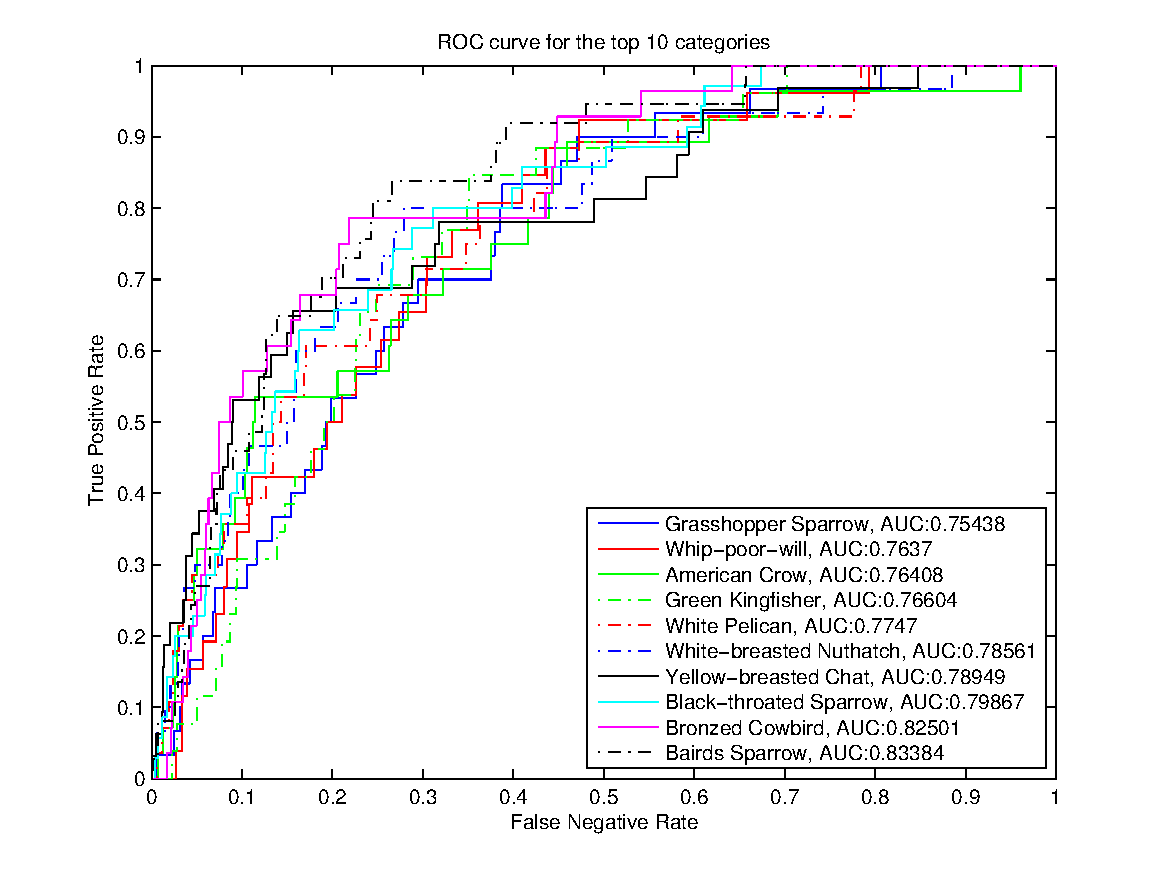
\includegraphics[width=1.1\linewidth,height=.75\linewidth]{birds_top10_ROC_final.eps}
%\vspace{-3mm}
\end{minipage}%
\hspace{-3mm}
\begin{minipage}{0.33\textwidth}
  \centering
 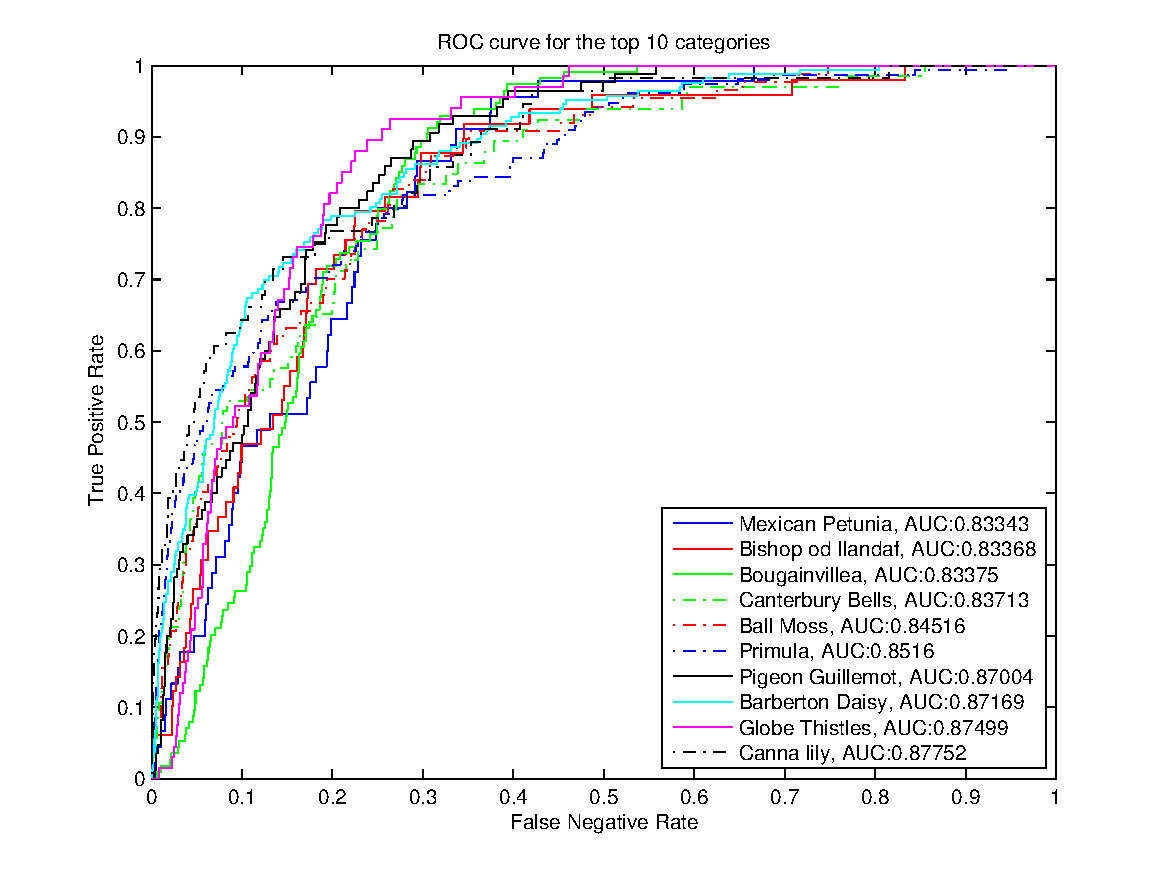
\includegraphics[width=1.1\linewidth,height=.75\linewidth]{flower_top10_ROC_final.eps}
 %\vspace{-3mm}
\end{minipage}
\begin{minipage}{0.33\textwidth}
  \centering
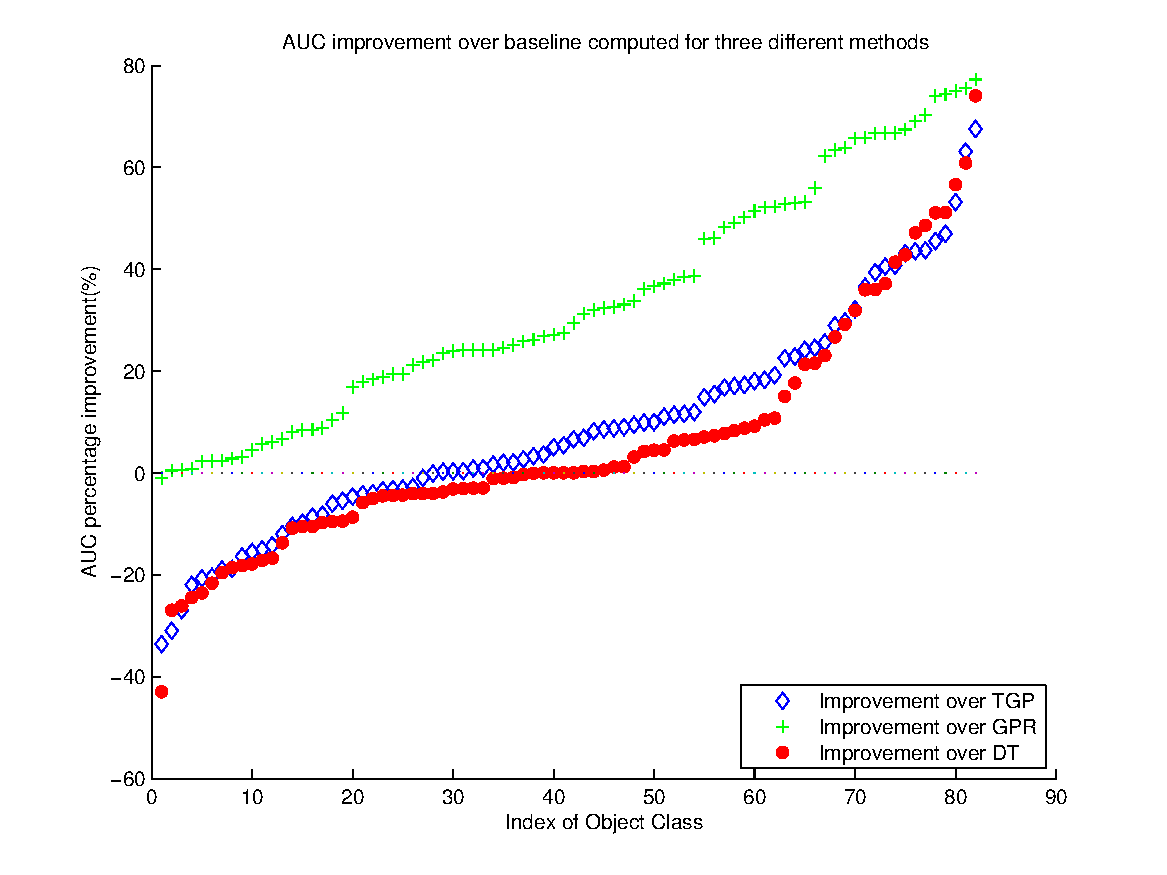
\includegraphics[width=1.1\linewidth,height=.75\linewidth]{flower_AUC_imp_final.eps}
%\vspace{-5mm}
\end{minipage}
\vspace{-1mm}
\caption{Linear : \textbf{Left and Middle}: ROC curves of best 10 predicted classes by the final formulation (E) for Bird  and Flower datasets respectively, \textbf{Right}: AUC improvement over the three baselines on Flower dataset (Formulations A (GPR), A (TGP), C). The improvement is sorted in an increasing order for each baseline separately (best seen in color)}
\vspace{-2mm}
\label{fig:result3fig}
\end{figure*}


\begin{table*}[b!]
\small
\centering
\caption{ Linear: Comparative Evaluation of Different Formulations on the Flower and Bird Datasets}
\label{T:AUC}
%\vspace{-10pt}
\scalebox{1.0}{
\begin{tabular}{|l|l|l|}
  \hline
  		&  Oxford Flowers   & UC-UCSD Birds   \\
  Approach  & Avg AUC (+/- std) & Avg AUC (+/- std)\\ 
  \hline
  \hline
  (A) Regression - GPR & 0.54 (+/- 0.02) & 0.52 (+/- 0.001) \\ 
  (A) Structured Regression - TGP & 0.58 (+/- 0.02) & 0.61 (+/- 0.02)\\
  (C)  Domain Transfer(DT) &  0.62(+/- 0.03)  &  0.59 (+/- 0.01)\\
  \hline 
  (B) Constrained GPR & 0.62(+/- 0.005) & - \\
  (B) Constrained TGP & 0.63(+/- 0.007) & - \\
  (D) Constrained Domain Adaptation (CDT) on Eq~\ref{eq:form} & 0.64 (+/- 0.006)& -  \\
       \hline
  (E) Regression+DT + constraints (final best linear approach) & {0.68} (+/- 0.01) & { 0.62} (+/- 0.02) \\
      \hline
\end{tabular}}
%\vspace{-10pt}
%\end{table}
%\begin{table}[t]
%\small
%\caption{\small Top-5 classes with highest combined improvement }
%\label{T:top5improv}
%\centering
%\vspace{-5pt}
\ignore{
{
\scalebox{0.7}{
\begin{tabular}{|l|l|l|l|l|}
  \hline
  \multicolumn{5}{c}{Top-5 Classes with highest combined improvement} \\
  \hline
  \hline
  class      &  (A) TGP (AUC) & (C) DT (AUC) & (D) TGP+DT+C  & \% Improv. \\
  \hline
  \hline
   2   &  0.51 & 0.55 & 0.83 & 57\% \\  
   28 & 0.52 & 0.54 & 0.76 &  43.5\% \\
   26 &  0.54 & 0.53 & 0.76 & 41.7\% \\
   81 & 0.52 & 0.82 & 0.87   & 37\%  \\
   37 & 0.72 & 0.53 & 0.83   & 35.7 \% \\
  \hline 
\end{tabular}}
}}
%\vspace{-5pt}
\end{table*}

\subsection{Experimental Results for Linear Classifier Prediction}


\noindent{\bf Evaluation Methodology:} Similar to zero-shot learning literature, we evaluated the performance of an unseen classifier in a one-vs-all setting where the test images of unseen classes are considered to be the positives and the test images from the seen classes are considered to be the negatives. We computed the ROC curve and report the area under that curve (AUC) as a comparative measure of different approaches. In zero-shot learning setting the test data from the seen class are typically very large compared to those from unseen classes. This makes other measures, such as accuracy, useless since high accuracy can be obtained even if all the unseen class test data are wrongly classified; hence we used ROC curves, which are independent of this problem. Five-fold cross validation over the classes were performed, where in each fold 4/5 of the classes are considered as ``seen classes'' and are used for training and 1/5th of the classes were considered as ``unseen classes'' where their classifiers are predicted and tested. Within each of these class-folds, the data of the seen classes are further split into training and test sets. The hyper-parameters for the  approach were selected through another five-fold cross validation within the class-folds  (i.e. the $80\%$ training classes are further split into $5$ folds to select the hyper-parameters). We made the seen-unseen folds used in our experiments available here \url{https://sites.google.com/site/mhelhoseiny/computer-vision-projects/Write_a_Classifier}.

\noindent{\bf Baselines:}
Since our work is the first to predict classifiers based on pure textual description, there are no other reported results to compare against. However, we designed three state-of-the-art baselines to compare against, which are designed to be inline with our argument in Sec~\ref{obvformulation}. Namely we used: 1) A Gaussian Process Regressor (GPR)~\cite{Rasmussen:2005}, 2) Twin Gaussian Process (TGP)~\cite{Bo:2010} as a structured regression method, 3)  Domain Transfer (DT)~\cite{da11}. The TGP and DT baselines are of particular importance since our formulation utilizes them, so we need to test if the formulation is making any improvement over them. It has to be noted that we also evaluate TGP and DT as alternative formulations that we are proposing for the problem, none of them was used in the same context before. %We  compared these baselines with formulations we proposed in section ~\ref{obvformulation} in including 4) Constrained GPR, 4) Constrained TGP, 5) Constrained DA, and 6) Constrained Regression  and Adaptation (our final approach).   

\begin{comment}
\begin{table}
\small
\centering
\caption{\small Comparative Evaluation on the Flowers and Birds}
\label{T:AUC}
%\vspace{-10pt}
\scalebox{1.0}{
\begin{tabular}{|l|l|l|}
  \hline
  		&  Flowers   & Birds   \\
  Approach  & Avg AUC (+/- std) & Avg AUC (+/- std)\\ 
  \hline
  \hline
  GPR  & 0.54 (+/- 0.02) & 0.52 (+/- 0.001) \\ 
  TGP  & 0.58 (+/- 0.02) & 0.61 (+/- 0.02)\\
  DT  &  0.62(+/- 0.03)  &  0.59 (+/- 0.01)\\
  Our Approach & {\bf 0.68} (+/- 0.01) & {\bf 0.62} (+/- 0.02) \\
  \hline 
\end{tabular}}
%\vspace{-10pt}
\end{table}

\end{comment}



\noindent{\bf Results:}
Table~\ref{T:AUC} shows the average AUCs for the final linear approach in comparison to the three baselines on both datasets. GPR performed poorly in all classes in both data sets, which was expected since it is not a structure prediction approach.  The DT formulation outperformed TGP in the flower dataset but slightly underperformed on the Bird dataset. The proposed approach outperformed all the baselines on both datasets, with significant difference on the flower dataset. It is also clear that the TGP performance was improved on the Bird dataset since it has more classes (more points are used for prediction). Fig ~\ref{fig:result3fig} shows the ROC curves for our approach on best predicted unseen classes from the Birds dataset on the Left  and Flower dataset on the middle. Fig ~\ref{F:AUCs} shows the AUC for all the classes on Flower dataset. %More results are attached in the supplementary materials. 
\begin{comment}
\begin{figure}
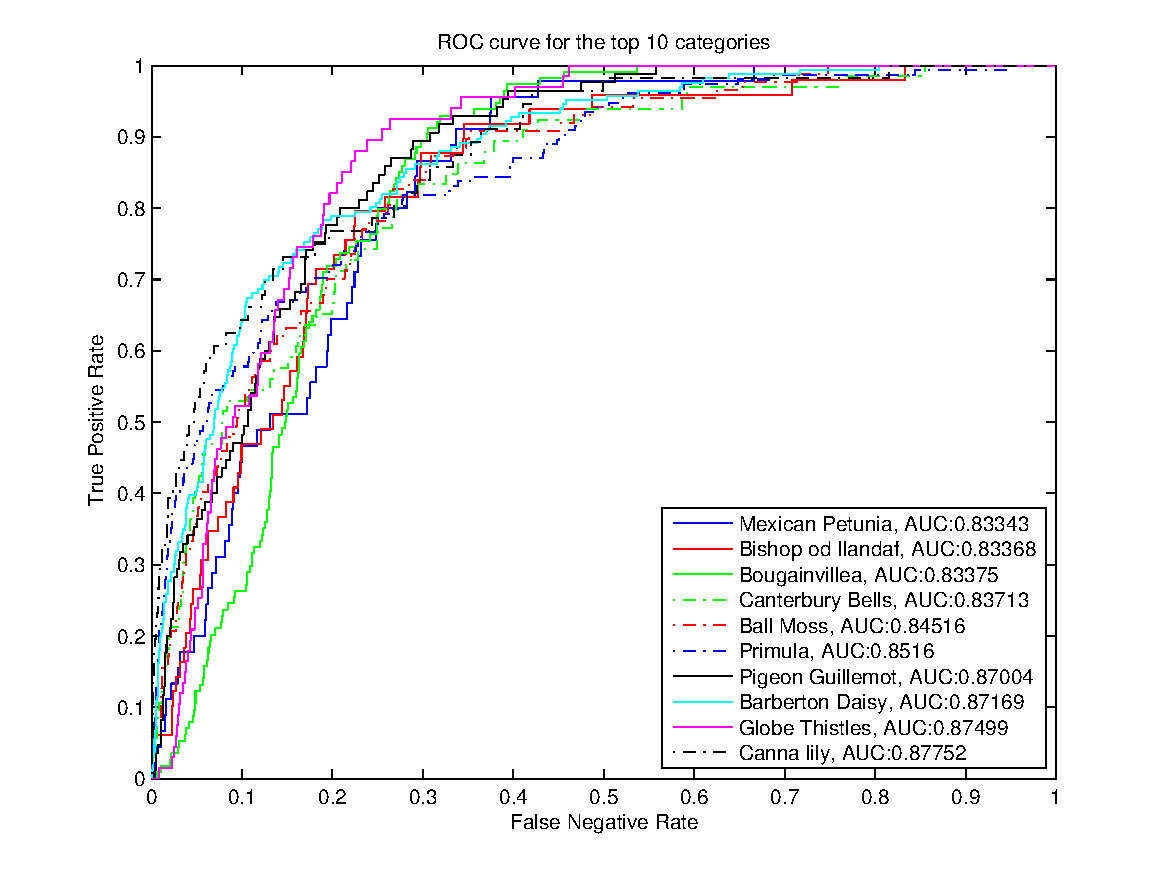
\includegraphics[width=0.9\linewidth,height=.6\linewidth]{flower_top10_ROC_final.eps}
%\vspace{-20pt}
\caption{ROC curves for best predicted classes -- Flower}
\label{F:bestROCs}
\end{figure}
\end{comment}
\begin{comment}
\begin{figure}
\centering
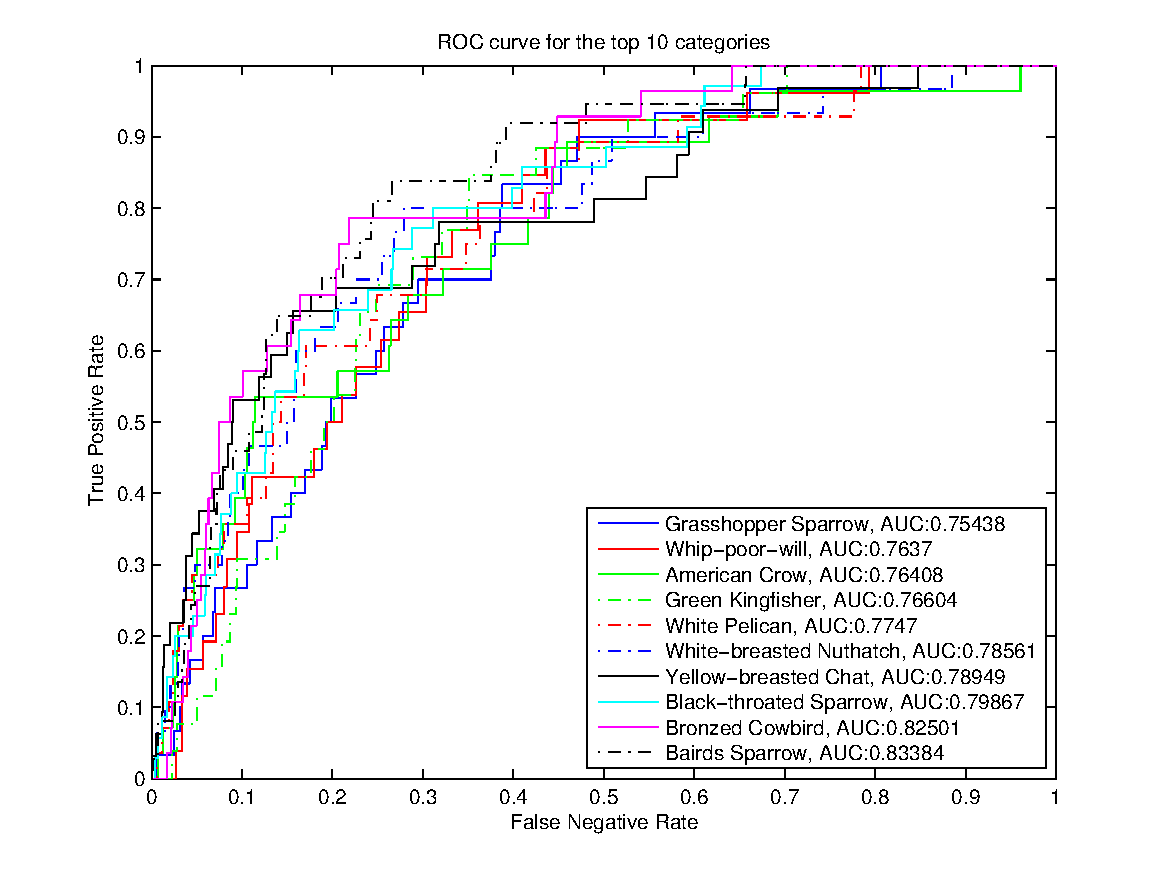
\includegraphics[width=0.8\linewidth,height=.5\linewidth]{birds_top10_ROC_final.eps}
%\vspace{-14pt}
\caption{ROC curves for best predicted classes -- Birds}
\label{F:bestROCsBIRDS}
%\vspace{-5pt}
\end{figure}
\end{comment}
\begin{comment}
\begin{figure}
\centering
\begin{minipage}{.45\textwidth}
  \centering
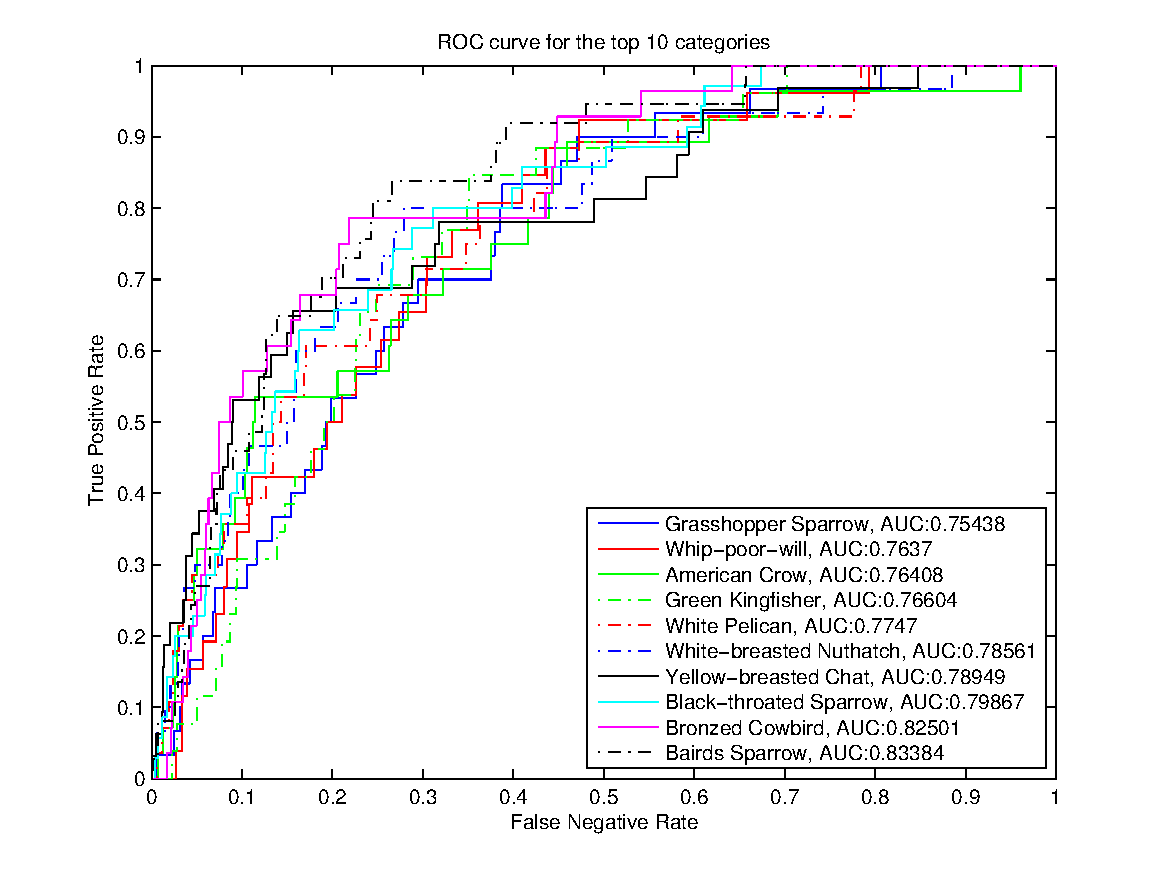
\includegraphics[width=0.43\linewidth,height=.4\linewidth]{birds_top10_ROC_final.eps}
	(a)
\end{minipage}%
\begin{minipage}{.45\textwidth}
  \centering
 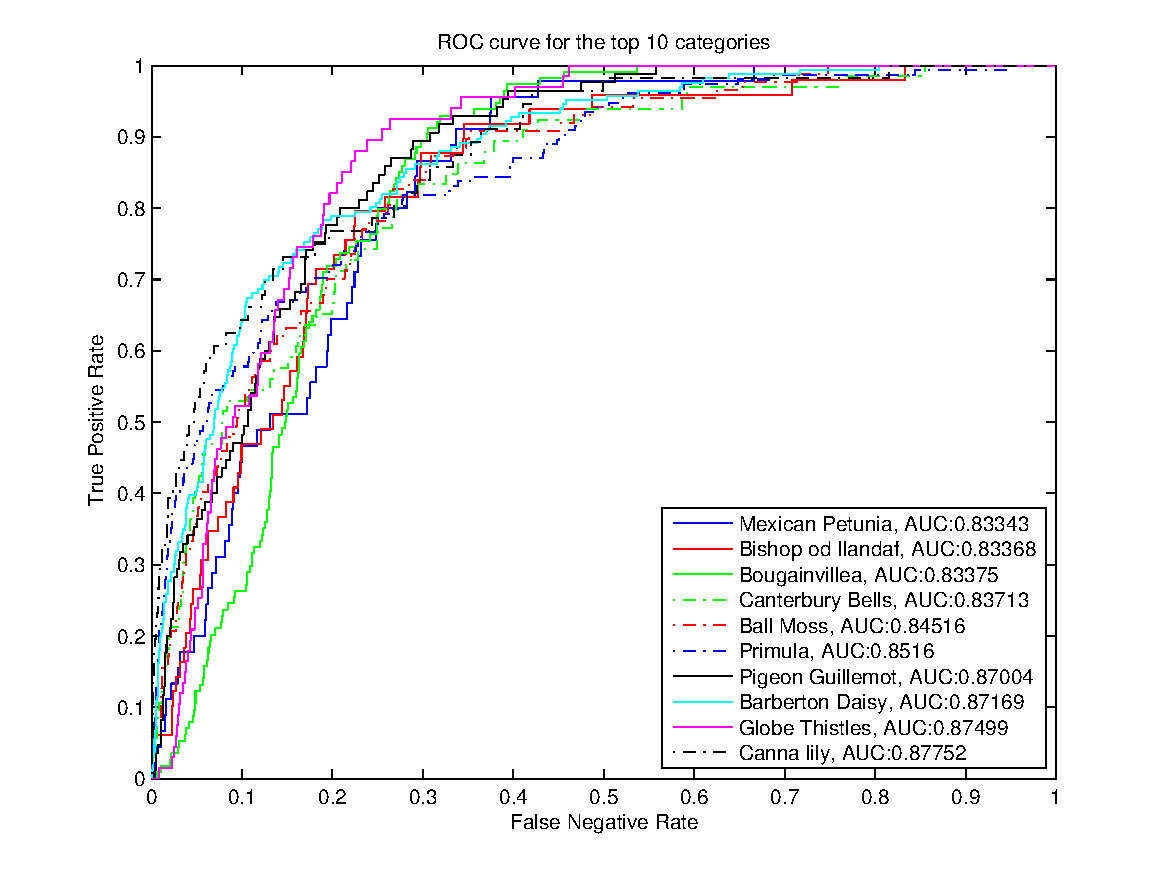
\includegraphics[width=0.43\linewidth,height=.4\linewidth]{flower_top10_ROC_final.eps}
 (b)
\end{minipage}
\end{figure}
\begin{figure}
        \begin{subfigure}[b]{0.45\textwidth}
                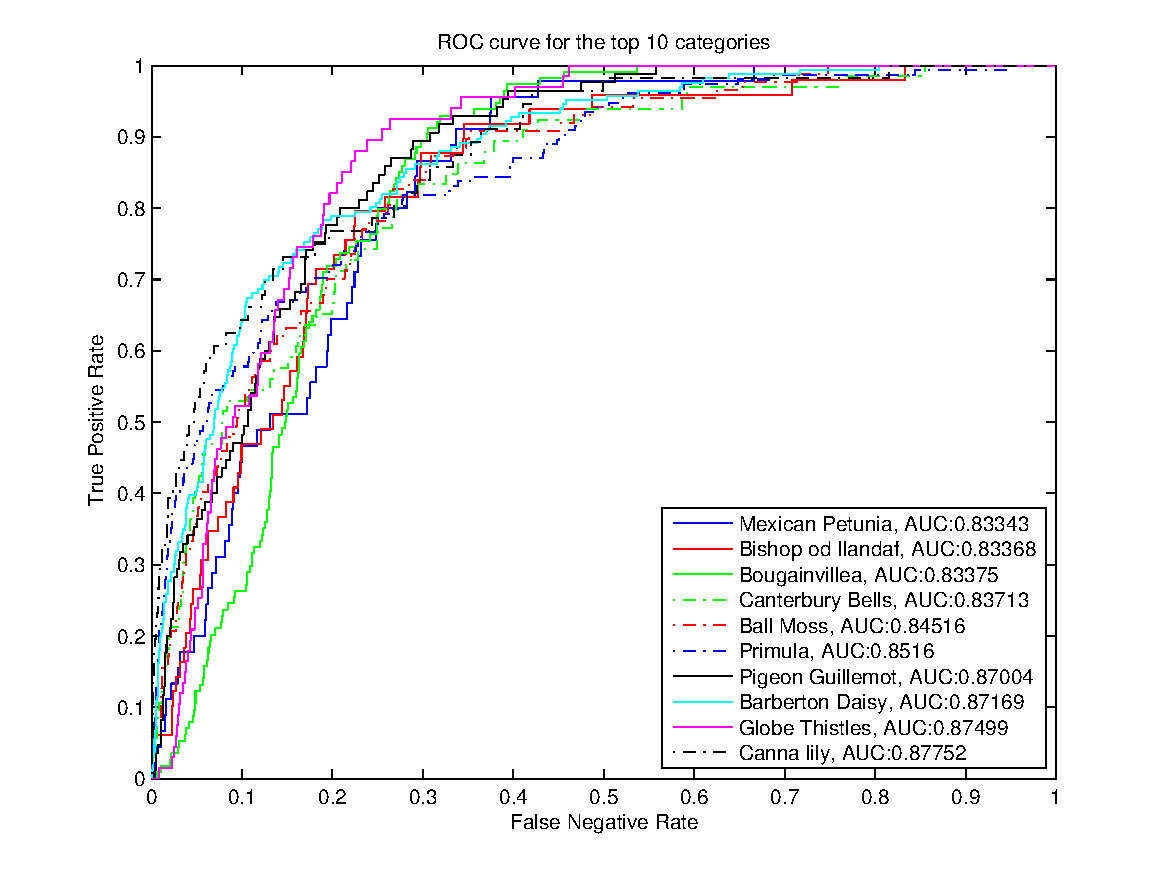
\includegraphics[width=0.4\linewidth,height=.4\linewidth]{flower_top10_ROC_final.eps}
                \caption{A gull}
                \label{fig:gull}
        \end{subfigure}\hspace{-20mm}
        \begin{subfigure}[b]{0.45\textwidth}
                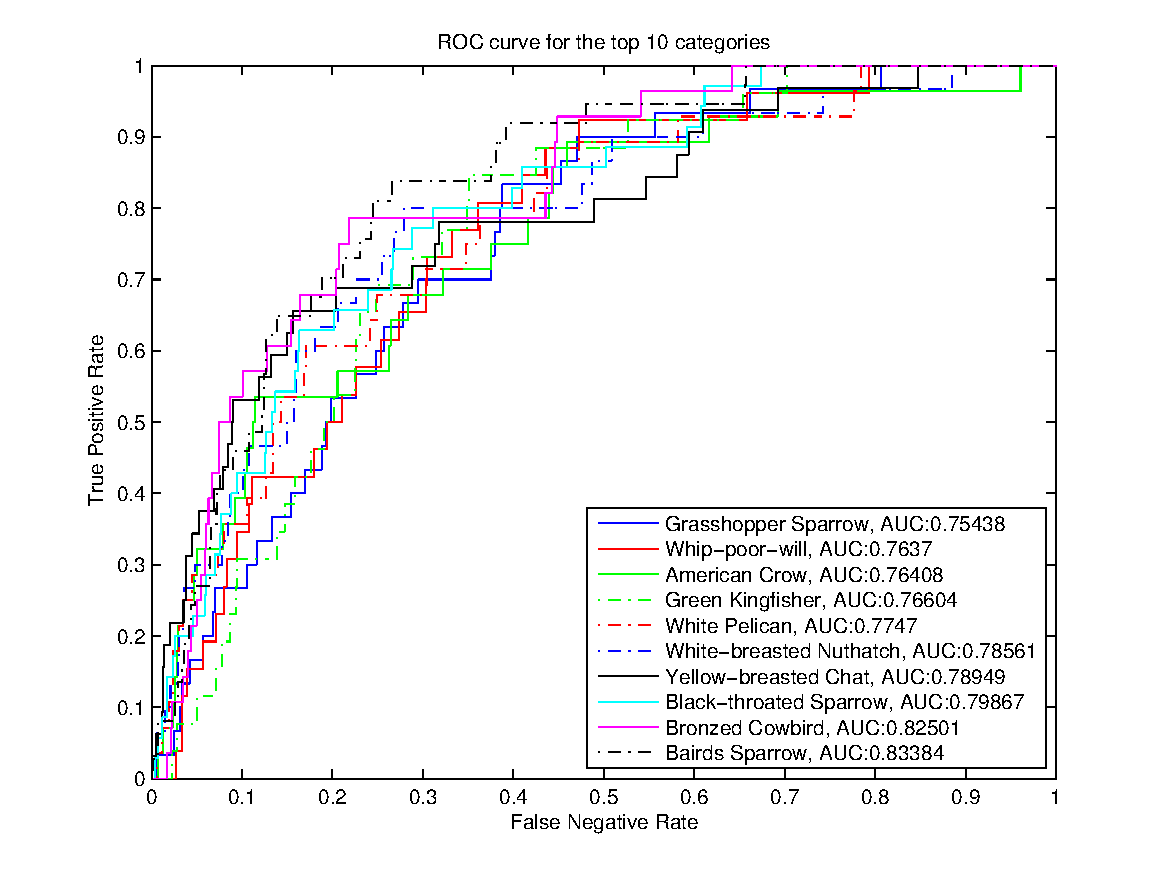
\includegraphics[width=0.4\linewidth,height=.4\linewidth]{birds_top10_ROC_final.eps}
                \caption{A tiger}
                \label{fig:tiger}
        \end{subfigure}
        \caption{Pictures of animals}
        \label{fig:animals}
\end{figure}
%\begin{center}
\end{comment}


%\end{center}



\begin{table}[t]
\small
\caption{\small Linear: Percentage of classes that the final proposed approach (formulation (E)) makes an improvement in predicting over the baselines (relative to the total number of classes in each dataset}
\label{T:classimprov}
%\vspace{-10pt}
\centering
\scalebox{1.0}{
\begin{tabular}{|l|l|l|}
  \hline
  		&  Flowers (102)  & Birds (200)\\ 
 baseline      &  \%  improvement & \%  improvement\\  
  \hline
  \hline
  (A) GPR  & 100 \% & 98.31 \% \\ 
  (A) TGP  & 66 \% & 51.81 \%\\
  (C) DT  &   54\% &  56.5\% \\
  %TGP+DA & 65\% &  55.45 \% \\
  \hline 
\end{tabular}}
%\vspace{-5pt}
\end{table}
\begin{comment}
\begin{figure}[t]
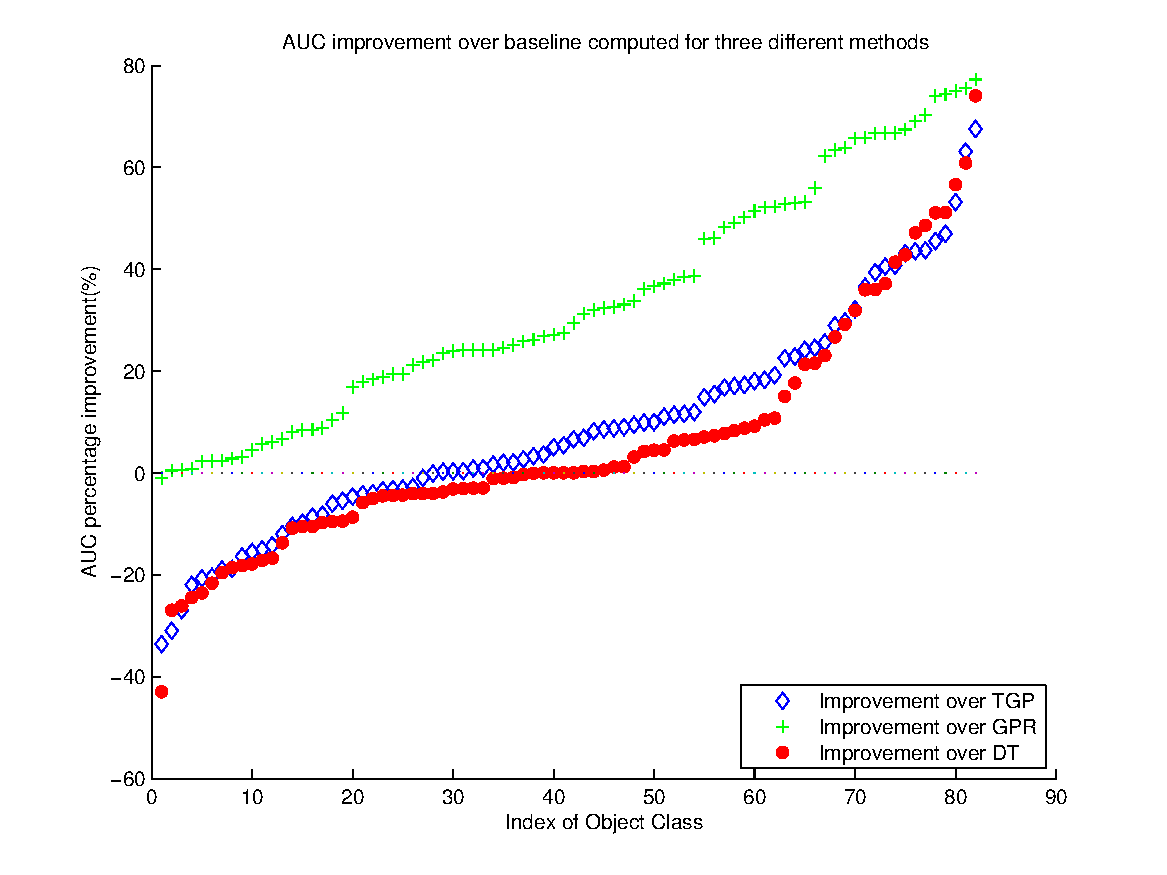
\includegraphics[width=0.95\linewidth,height=.5\linewidth]{flower_AUC_imp_final.eps}
%\vspace{-10pt}
\caption{AUC improvement over the three baselines. The improvement are sorted in a decreasing order for each baseline separately. }
\label{F:AUC_improvement}
\end{figure}
\end{comment}
Fig ~\ref{fig:result3fig}, on the right, shows the improvement over (A) GPR,\begin{figure}
\vspace{-3mm}
\centering
 \hspace*{-12mm}%
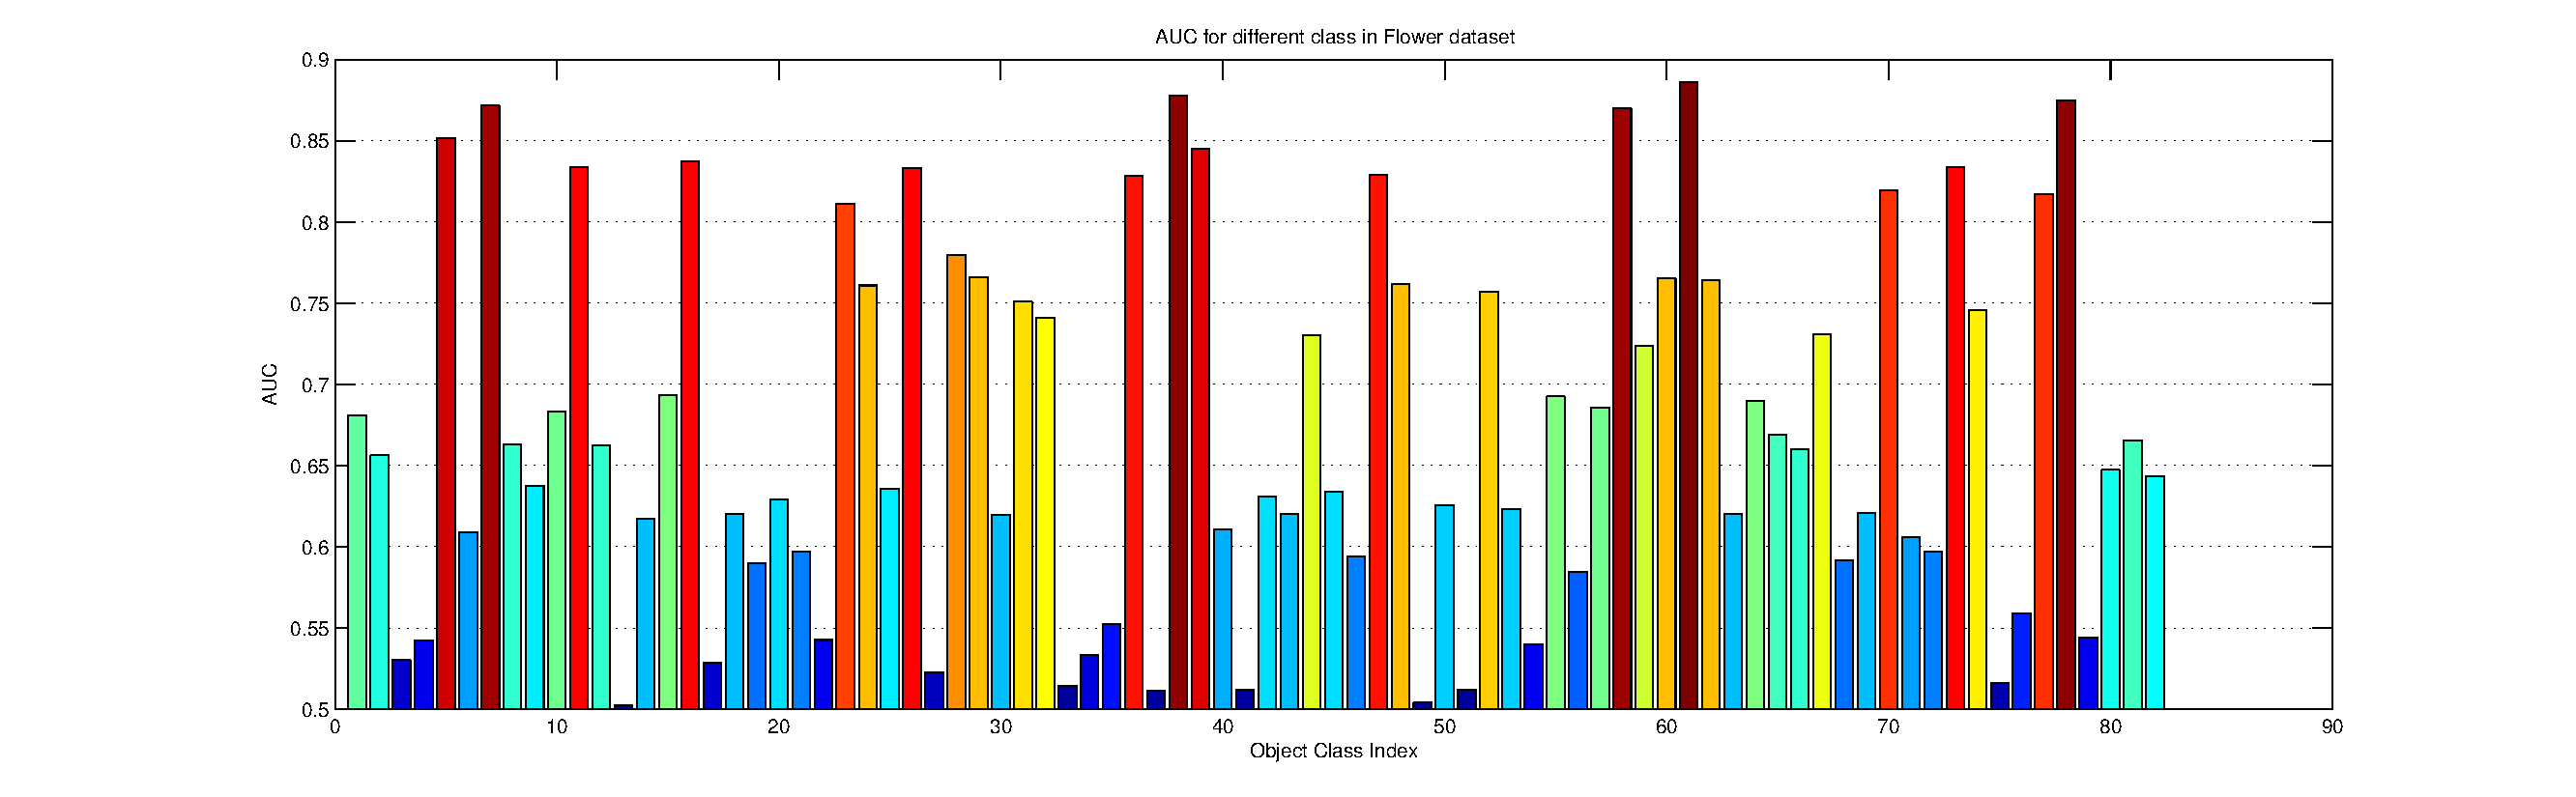
\includegraphics[width=1.24\linewidth,height=.27\linewidth]{flower_AUC_for_all_classes_final.eps}
%\vspace{-15pt}
\caption{Linear: AUC of the predicated classifiers for all classes of the flower datasets (Formulation E)}
\label{F:AUCs}
\end{figure} A(TGP), and (C) DT for each class, where the improvement is calculated as (our AUC- baseline AUC)/ baseline AUC \%. 
Table~\ref{T:classimprov} shows the percentage of the classes which our approach makes a prediction improvement for each of  the three baselines\begin{comment}. The last row show the improvement over both the TGP and DT baseline 
\end{comment}
. Table~\ref{T:top5improv} shows the five classes in Flower dataset where our approach made the best average improvement.
\begin{comment}. (TGP+DT).  
\end{comment}
 The point of that table is to show that in these cases both TGP and DT did poorly while our formulation that is based on both of them did significantly better. This shows that our formulation does not simply combine the best of the two approaches but can significantly improve the prediction performance.

\begin{table}[t]
\small
\caption{\small Linear: Top-5 classes with highest combined improvement in Flower dataset}
\label{T:top5improv}
\centering
%\vspace{-5pt}
{
\scalebox{0.85}{
\begin{tabular}{|l|l|l|l|l|}
  \hline
  class      &  (A) TGP (AUC) & (C) DT (AUC) & (E) Our (AUC)  & \% Improv. \\
  \hline
  \hline
   2   &  0.51 & 0.55 & 0.83 & 57\% \\  
   28 & 0.52 & 0.54 & 0.76 &  43.5\% \\
   26 &  0.54 & 0.53 & 0.76 & 41.7\% \\
   81 & 0.52 & 0.82 & 0.87   & 37\%  \\
   37 & 0.72 & 0.53 & 0.83   & 35.7 \% \\
  \hline 
\end{tabular}}
}
\vspace{-2pt}
\end{table}







To evaluate the effect of the constraints in the objective function, we removed the constraints $- (\mathbf{c}^\textsf{T} {\mathbf{x}}_{i} ) \geq \zeta_i$ which try to enforces all the seen examples to be on the negative side of the predicted classifier hyperplane and evaluated the approach. The result on the flower dataset (using one fold) was reduced to average AUC=0.59 compared to AUC=0.65 with the constraints. Similarly, we evaluated the effect of the constraint  $\mathbf{t}_*^\textsf{T} \mathbf{W} \mathbf{c} \ge l$. The result was reduced to average AUC=0.58 compared to AUC=0.65 with the constraint.  This illustrates the importance of this constraint in the formulation.

\noindent{\bf Constrained Baselines:}
%\textbf{different formulations experiments:}
\ignore{We computed the ROC curves and report the area under that curve (AUC) as a comparative measure\footnote{In zero-shot learning setting the test data from the seen class are typically very large compared to those from unseen classes. This makes other measures, such as accuracy, useless since high accuracy can be obtained even if all the unseen class test data are wrongly classified; hence we used ROC curves, which are independent of this problem.} Five-fold cross validation over the classes were performed, within each of these class-folds, the data of the seen classes are further split into training and test sets.}
Table~\ref{T:AUC} (bottom three lines) also shows the average AUCs for the constrained baselines formulations, namely Constrained GPR, TGP and DT; see section~\ref{formulation}. Even though the visual features and textual features were independently extracted, by learning correlation between them, we can predict classifiers for new categories. As shown previously, GPR performed poorly, while, as expected, TGP performed better. Adding constraints to GPR/TGP improved their performance. Combining regression and DT gave significantly better results for classes where both approaches individually perform poorly, as can be seen in Table~\ref{T:AUC}-right. We performed an additional experiment, where  $\mathbf{W}$ is firstly computed using Constrained Domain Transfer (CDT). Then, the unseen classifier is predicted using equation~\ref{eq:form} with $\gamma=0$, which performs worse. This indicates that adding constraints to align to seen classifiers hurts the learnt domain transfer function on unseen classes. In conclusion, the final formulation that combines TGP and DT with additional constraints performs the best in both Birds and Flower datasets, where the effect of TGP is very limited since it was trained on sparse points. 

%\begin{float}





\subsection{Experimental Results for Kernel Classifier Prediction}
\label{ss_exp_kernel}


%!TEX root = ZeroShotLearningECCV14.tex
\ignore{
Now that we have described our zero-shot learning setting and the suggested approaches to directly predict kernel-classifier parameters for unseen classes, we present several experiments to validate our model.
}
\ignore{In this section, we presented a set of experiments, conducted to evaluate our proposed model for zero-shot learning of visual classifiers. The quantitative comparisons show our superior performance to the state of the art on two challenging datasets of fine-grained object categories.}
%\subsection{Datasets}


%We performed three experiments to validate our model on two challenging fine-grained recognition datasets. Two of experiments were performed on UCSD-Birds dataset \cite{CU20010}, while the remaining one was performed on Oxford-Flower dataset \cite{Flower08}. UCSD-Birds dataset consists of 200 classes, total of 6033 images. On the other hand, the Flower dataset consists of 102 flower categories, and total of 8189 images. For the first two experiments, we used the textual descriptions' augmentation provided by  for Birds and Flower datasets,  as privileged information provided for each class description. In the third experiment, we used the average attribute vector of each class in Birds dataset as privileged information. Unlike typical attribute-based approaches, that learn attribute classifiers as an intermediate representation, our approach does not need to learn any attribute classifiers. Next subsections details the experimental settings and the features.

\subsubsection{Additional Evaluation Metrics}

In addition to the the AUC, we already studied in the previous section. We report two additional metrics while evaluating and comparing the kernel classifier prediction to the linear classifier prediction, detailed as follows. 

%\textit{AUC:}  In order to measure the discriminative ability of our predicted one-vs-all classifier for each unseen class, against the seen classes, we report the area under the ROC curve. \ignore{This is because a large accuracy could be achieved even if all unseen points are incorrectly classified.} Since unseen class positive examples are few compared to negative examples, a large accuracy could be achieved even if all unseen points are incorrectly classified. Hence, AUC is a more consistent measure, compared to accuracy for this purpose.  In this setting, we use the predicted classifier of an unseen class as a binary separator against the seen classes. This measure is computed for each predicted unseen classifier and the average AUC is reported as well. This is the only measure addressed in \cite{Hoseini13} to evaluate the unseen classifiers, which is limiting in our opinion. Instead, we cover the following additional metrics to evaluate explicit classifier prediction. 

\textit{\small$|N_{sc}|\,$\normalsize to \small$|N_{sc}+1|\,$\normalsize Recall:}
Under this metric, we aim to check  how   the learned classifiers of the seen classes confuse the predicted classifiers, when they are involved in a multi-class classification problem of \small$N_{sc} + 1\,$\normalsize classes. \ignore{The first \small$N_{sc}\,$\normalsize classifiers are those of the seen classes, while \small$({N_{sc}+1})^{st}$\normalsize classifier is a predicted classifier for an unseen class. }We use Eq~\ref{eq:mclass} to predict label $l^*$  with the maximum confidence of an image \small$x^*$\normalsize, such that \small$l^* \in {L}_{sc} \cup l_{us}$\normalsize,  \small$l_{us}\,$\normalsize is the label of the ground truth unseen class, and ${L}_{sc}$ is the set of seen class labels. We compute the recall under this setting. This metric is computed for each predicted unseen classifier and the average is reported.

\textit{Multiclass Accuracy of Unseen classes (MAU):} Under this setting, we aim to evaluate the performance of  the unseen  classifiers against each others. Firstly, the classifiers of all unseen categories are predicted. Then, we use Eq~\ref{eq:mclass} to predict the label with the maximum confidence of a test image $x$, such that its label $l_{us}^* \in {L}_{us}$, where ${L}_{us}$ is the set of all unseen class labels that only have text descriptions. 



%Table~\ref{tab:settings} shows the settings of the three experiments, we performed on Flower and Birds datasets, where $|{Y}_{sc}|$ and $|{Y}_{us}|$ are the number of the seen and the unseen classes, respectively. In these experiments $\mathcal{D}_{train} =\{ \mathcal{S}_x = \{(\textbf{x}_i,y_i)\}_N , \mathcal{S}_e = \{ y_i, \textbf{e}_i\}_{N_{sc}} \}$ involves $80\%$ of the classes in the dataset, and $D_{test} = \{ \mathcal{S}_x^*= \{ \textbf{x}^*_j \}_{N'}, \mathcal{S}_e^* = \{ y^*_j, \textbf{e}_{y^*_j} \}_{N_{us}} \}$ involves $20\%$ of the classes in the dataset. This data split is applied for both Birds and Flower datasets, as illustrated in Table ~\ref{tab:settings}.

%\begin{table}[h!]
%\caption{The experimental settings}
%\label{tab:settings}
%\centering
%\begin{tabular}{|c|c|c|c|c|c|}
%\hline 
% & Dataset & $\mathcal{E}$ domain & $\mathcal{X}$ domain & $|\mathcal{Y}_{sc}|$ & $|\mathcal{Y}_{us}|$ \\ 
%\hline 
%Expr 1 & Flower & text  & classeme & 80 & 22 \\ 
%\hline 
%Expr 2 & Birds & attributes & classeme & 160 & 40 \\ 
%\hline 
%Expr 3 & Birds & text & classeme & 160 & 40 \\ 
%\hline 
%\end{tabular} 
%\end{table}




\subsubsection{Comparisons to Linear Classifier Prediction}
\label{exp1}
 We compare the kernel methods to the linear prediction discussed earlier,  which predicts a linear classifier from textual descriptions  ( \small$\mathcal{T}\,$\normalsize space in our framework). The aspects of the comparison includes  1) whether the predicted kernelized classifier outperforms the predicted linear classifier  2) whether this behavior is consistent on multiple datasets. We performed the comparison on both Birds and Flower dataset.  For these experiments, in our setting, domain \small$\mathcal{V}\,$\normalsize is the visual domain and domain \small$\mathcal{T}\,$\normalsize is the textual domain, \ie, the goal is to predict classifiers from pure textual description. We used the same features on the visual domain  and the textual domains detailed in subsection~\ref{ss_ds_feats}. That is,  classeme features \cite{classemes} for images, extracted from images of the Bird and the Flower datasets and tf-idf~\cite{salton1988term} features for text articles followed by a CLSI~\cite{clsi05} dimensionality reduction phase. %Classeme  is a 2569-dimensional features, which correspond to confidences of a set of one-vs-all classifiers, pre-trained on images from the web, as explained in~\cite{classemes}, not related to either the Bird nor the Flower datasets. The rationale behind using these features in~\cite{Hoseini13} was that they offer a semantic representation\ignore{ represent semantic-level features, which would have better chance in correlating with the textual features}.
  %For the textual domain, we used the same textual feature extracted by~\cite{Hoseini13}. In that work, 
 %tf-idf (Term-Frequency Inverted Document Frequency)\cite{salton1988term} features were extracted from the textual articles were used, followed by a CLSI~\cite{clsi05} dimensionality reduction phase.
 
We denote our kernel Domain Transfer prediction  and one class SVM adjust DT prediction by  ``DT-kernel'' and ``SVM-DT-kernel'' respectively. We compared against  linear classifier prediction (Linear Formulation (E) approach, denoted by just Linear Classifier).  \ignore{(which uses a quadratic program to optimize the classifier parameters)}We also compared against the  linear direct domain transfer (Linear Formulation (C), denoted by DT-linear).  In our kernel approaches, we used Gaussian rbf-kernel as a similarity measure in \small$\mathcal{T}\,$\normalsize and \small$\mathcal{V}\,$\normalsize spaces (\ie \small$k(d,d') = exp(-\lambda ||d-d'||)$\normalsize). 

 
%\textbf{Text features as $\mathcal{E}$  (Expr1 [Flower], Expr2 [Birds] )}
%We start by presenting AUC an MAU metrics on Flower and Birds dataset, we follow that by an argument on  the results.
\begin{table*}[hb!]
\vspace{-1mm}
 \begin{minipage}{0.56\linewidth}
\caption{Kernel: Recall, MAU, and average AUC on three seen/unseen splits on Flower Dataset and a seen/unseen split on Birds dataset}
\label{tbl:flowerbirdsmauauc}
  \centering
  \scalebox{0.90}
  {
\begin{tabular}{|c|c|c|c|c|}
\hline 
  & \textbf{Recall-Flower} & improvement & \textbf{Recall-Birds}& improvement \\ 
  \hline 
{SVM-DT kernel-rbf }& \textbf{40.34\% (+/-  1.2) \%} & & \textbf{44.05 \%}   &  \\ 
\hline 
Linear Classifier  & 31.33  (+/-  2.22)\% & 27.8 \%  & 36.56 \% & 20.4 \% \\ 
\hline 
\end{tabular}}

\hspace{-1.5mm}\scalebox{0.943}
  {
\begin{tabular}{|c|c|c|c|c|}
\hline 
  & \textbf{MAU-Flower} & improvement & \textbf{MAU-Birds}& improvement \\ 
  \hline 
{SVM-DT kernel-rbf }& \textbf{9.1 (+/-  2.77) \%} & & \textbf{3.4  \%}   &  \\ 
\hline 
{DT kernel-rbf }& \textbf{6.64 (+/-  4.1) \%} & 37.93 \%  & \textbf{2.95  \%} & 15.25 \% \\ 
\hline 
Linear Classifier \ignore{ Prediction} & 5.93  (+/-  1.48)\% & 54.36 \%  & 2.62 \% & 29.77 \% \\ 
\hline 
DT-linear\ignore{~\cite{Hoseini13,da11}} & 5.79 (+/-  2.59)\% & 58.46 \%  &  2.47 \% & 37.65 \%  \\ 
\hline 
\end{tabular}}
\scalebox{0.93}
  {
\begin{tabular}{|c|c|c|c|c|} 
\hline 
 & \textbf{AUC-Flower}& improvement & \textbf{AUC-Birds} & improvement\\ 
\hline 
{SVM-DT kernel-rbf }& {0.653 (+/-  0.009) } &   &   0.61  &   \\ 
\hline 
{DT kernel-rbf }& {0.623 (+/-  0.01) \%} & 4.7 \% &  0.57  & 7.02 \%  \\ 
\hline 
Linear Classifier \ignore{Prediction} & 0.658 (+/-  0.034) & - 0.7 \% & 0.62  & -1.61\%  \\ 
\hline 
Domain Transfer\ignore{~\cite{Hoseini13,da11}} &0.644 (+/-  0.008) &  1.28 \% & 0.56  & 8.93\%  \\ 
\hline 
\end{tabular} 
}
%\vspace{-5mm}
\end{minipage}
 \begin{minipage}{00.02\linewidth}
 $\,\,$
 \end{minipage}
\begin{minipage}{0.42\linewidth}
\centering
   \caption{Kernel: MAU on a seen-unseen split-Birds Dataset (MKL)}
\label{tbl:birdsmkl}
 \scalebox{0.93}
  {
\begin{tabular}{|c|c|c|}
\hline 
& MAU & improvement \\ 
\hline 
{SVM-DT kernel-rbf (text)}& \textbf{4.10  \%} &   \\ 
\hline 
Linear Classifier \ignore{Prediction} & 2.74 \% & 49.6 \% \\ 
\hline 
\end{tabular} }

\centering
     \vspace{5mm}
   \caption{Kernel: MAU on a seen-unseen split-Birds Dataset (CNN image features, text description)}
     %\vspace{-1mm}
\label{tbl:birdscnn}
 \scalebox{0.93}
  {
\begin{tabular}{|c|c|c|}
\hline 
& MAU & improvement \\ 
\hline 
\hline 
{SVM-DT kernel ($\mathcal{V}$-rbf, $\mathcal{T}$-DS kernel)}& \textbf{5.35  \%} &   \\ 
\hline
{SVM-DT kernel ($\mathcal{V}$-rbf, $\mathcal{T}$-rbf on TFIDF)}& \textbf{4.20  \%} &  27.3\% \\ 
\hline 
Linear Classifier (TFIDF text) \ignore{Prediction} & 2.65 \% & 102.0\% \\ 
\hline 
\cite{norouzi2014zero} & 2.3\% & 132.6\% \\
\hline 
\end{tabular} }
 %\vspace{-5mm}
\end{minipage}
\vspace{-4mm}
\end{table*}




\textit{Recall metric : } The recall of the SVM-DT kernel approach is 44.05\% for Birds and 40.34\% for Flower, while it is 36.56\% for Birds and  31.33\% for Flower by best Linear Classifier prediction (E). This indicates that the  predicted classifier is less confused by the classifiers of the seen compared with  Linear Classifier prediction; see table ~\ref{tbl:flowerbirdsmauauc} (top part)


\textit{MAU metric:} It is worth to mention that the multiclass accuracy for the trained seen classifiers is $51.3\%$ and $15.4\%$, using the classeme features,  on Flower dataset and Birds dataset\footnote{Birds dataset is known to be a challenging dataset for fine-grained, even when applied in a regular multiclass setting as it is clear from the $15.4\%$ performance on seen classes}, respectively. Table ~\ref{tbl:flowerbirdsmauauc} (middle part) shows the average $MAU$ metric over three seen/unseen splits for Flower dataset and one split on Birds dataset, respectively. 
Furthermore, the relative improvements of our  SVM-DT-kernel approach is reported against the baselines. On Flower dataset,  it is interesting to see that our approach achieved $9.1\%$ MAU, $182\%$ the random guess performance, \ignore{, which is $17.7\%$ of the multi-class accuracy of the seen classes (i.e. $51.3\%$),} %\footnote{$17.7 = 9.1 / 51.3 \cdot 100$}
by predicting the unseen classifiers using just textual features as privileged information (i.e. $\mathcal{T}$ domain). It is important to mention that we achieved also $13.4\%$, $268\%$ the random guess performance, in one of the splits (the 9.1\% is the average over 3 seen/unseen splits). Similarity on Birds dataset, we achieved $3.4\%$ MAU from text features, $132\%$  the random guess performance (further improved up to $224\%$ in next experiments).\ignore{, which is $22.7\%$ of the multi-class accuracy of the seen classes on the same dataset ($15.4\%$)}


\textit{AUC metric: } Fig\ignore{~\ref{F:top10} }~\ref{F:AUCstop10} (top part) shows the ROC curves for our approach on the best predicted unseen classes from the Flower dataset. Fig\ignore{~\ref{F:AUCs}}~\ref{F:AUCstop10} (bottom part) shows the AUC for all the classes on Flower dataset (over three different splits). Table~\ref{tbl:flowerbirdsmauauc} (bottom part)  shows the average AUC on the two datasets, compared to the baselines. More results and figures \ignore{Corresponding figures for Birds dataset } for our kernel approach are attached in the supplementary materials.

Looking at table~\ref{tbl:flowerbirdsmauauc}, we can notice that the proposed approach performs marginally similar to the baselines from AUC perspective. However, there is a clear improvement  in MAU  and Recall metrics. These results show the advantage of predicting classifiers in kernel space. Furthermore, the table shows that our SVM-DT-kernel approach outperforms our DT-kernel model. This indicates the advantage of the class separation, which is adjusted by the SVM-DT-kernel model. \ignore{In all these experiments, we used a setting of our SVM-DT-kernel model, where \small$C_{\beta}({ \textbf{T}} )\,$\normalsize is ignored (i.e. \small$\lambda_2 = 0$\normalsize)\ignore{; see Sec ~\ref{ss:tr}}). In order to study whether \small$C_{\beta}( \textbf{T} )\,$\normalsize is effective in unseen class prediction, we performed an extra experiment on Birds dataset, where \small$\lambda_2>0\,$\normalsize (e.g. \small$\lambda_2 =1$\normalsize). We found that MAU of our DT approach has slightly decreased (i.e from $2.95\&$  to $2.91\%$ ). Under the same setting, we also found that  \small$C_{\beta}( \textbf{T} )\,$\normalsize  slightly reduced the performance of SVM-DT from $9.1\%$ to $8.98\%$.MAU. This reflect our intuition argued in the approach section\ignore{Sec ~\ref{ss:tr}}. Hence, we suggest to assign \small$\lambda_2\,$\normalsize to $0$ for our purpose.} More details on the hyper-parameter selection are attached in the supplementary materials. 
\begin{figure}[t!]
 \centering
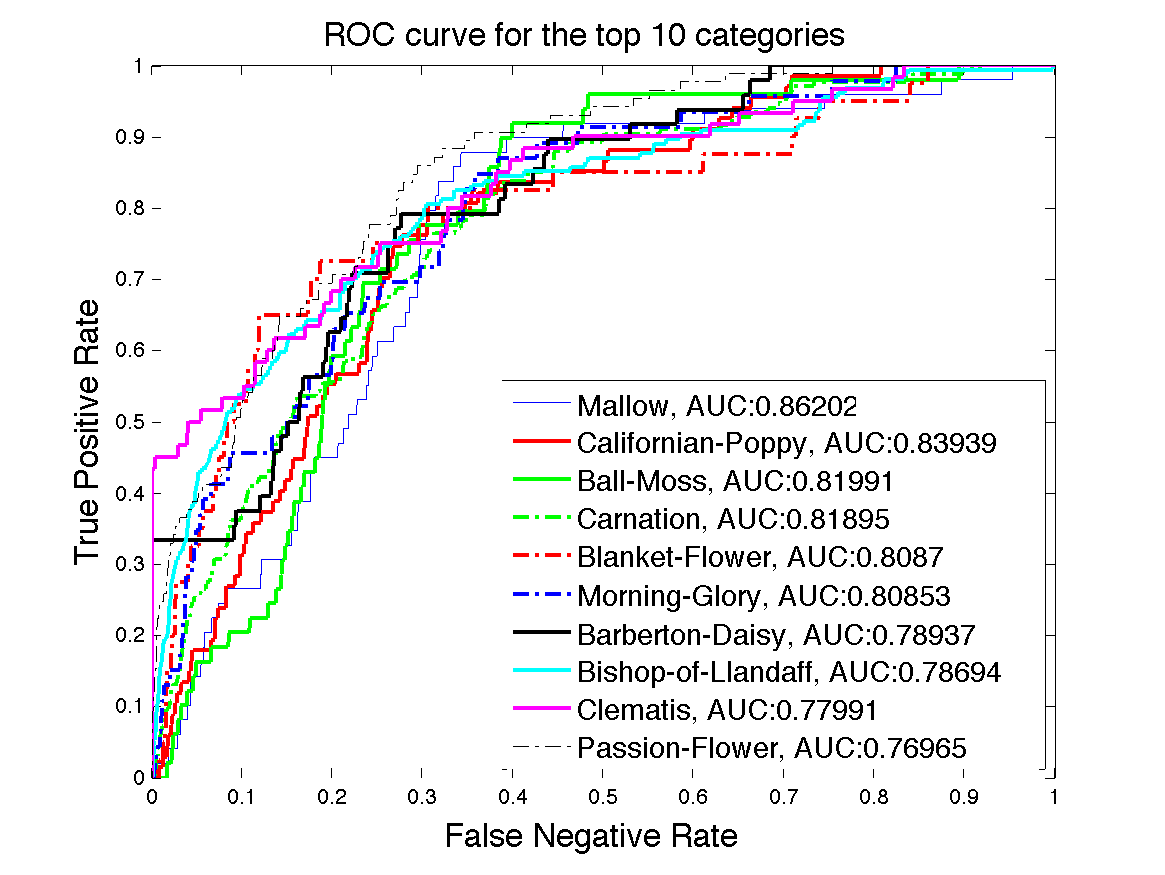
\includegraphics[width=1.00\linewidth,height=.66\linewidth]{figroc.eps}
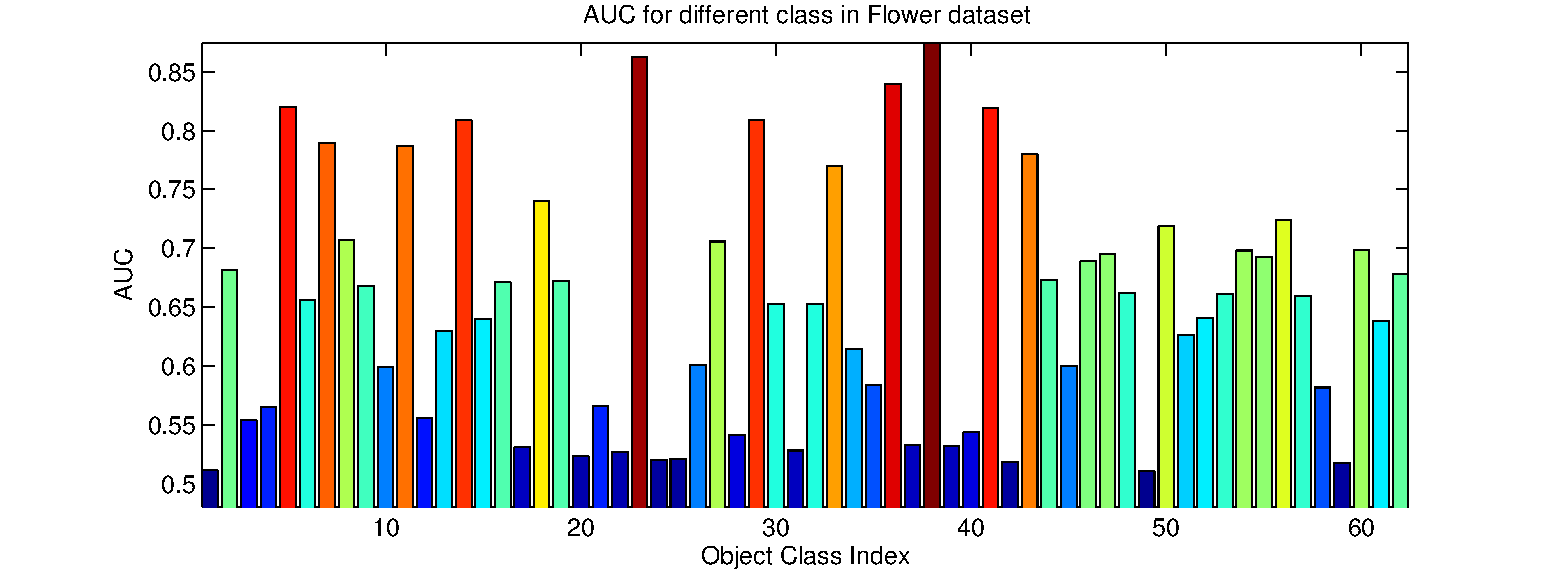
\includegraphics[width=1.00\linewidth,height=.34\linewidth]{fig1auc.eps}
%\caption{ROC-curves for the top 10 classifiers in Flower dataset}
%\vspace{-2mm}
\caption{Kernel: AUC of the 62 unseen classifiers the flower data-sets over three different splits (bottom part) and their Top 10 ROC-curves (top part)}
%\vspace{-2mm}
\label{F:AUCstop10}
\end{figure}








\begin{comment}
\begin{figure}[h!]
\centering
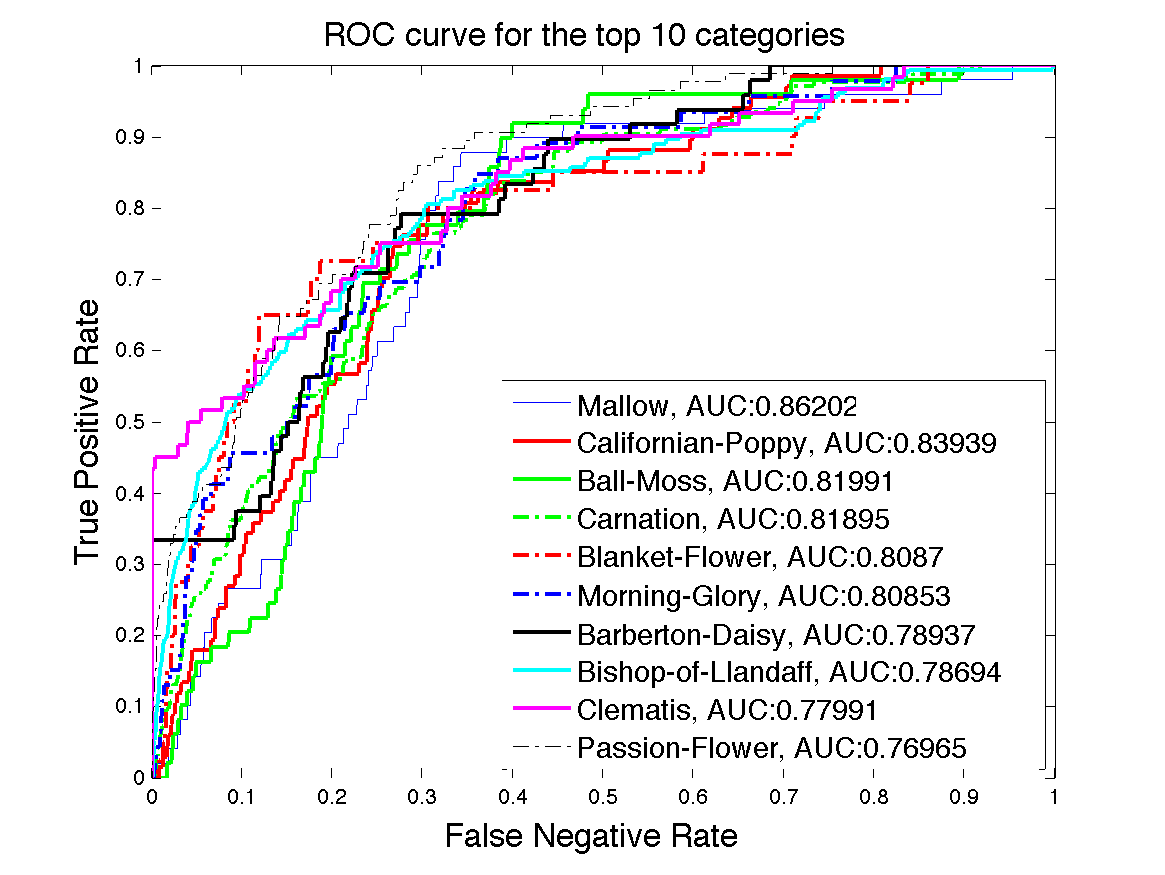
\includegraphics[width=0.7\linewidth,height=.50\linewidth]{figroc.eps}
\caption{ROC-curves for the top 10 classifiers in Flower dataset}
\label{F:top10}
\end{figure}



\begin{figure}[h!]
\centering
 \hspace*{-12mm}%
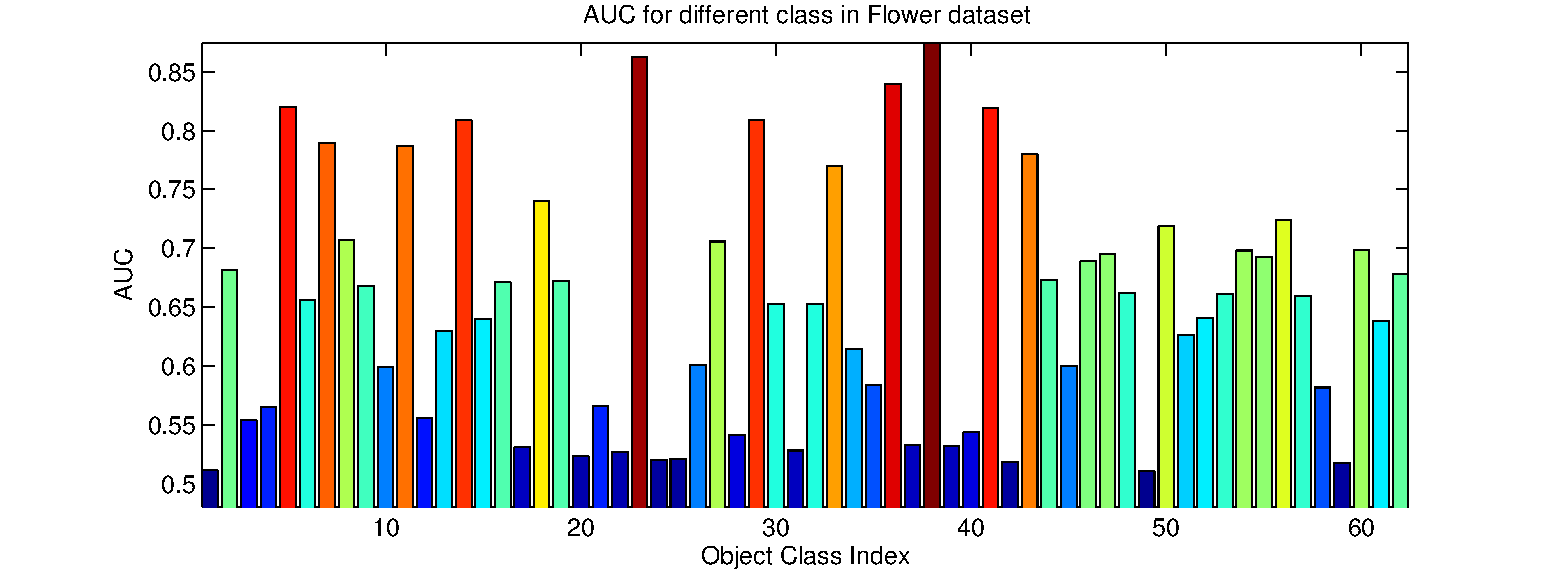
\includegraphics[width=1.0\linewidth,height=.30\linewidth]{fig1auc.eps}
%\vspace{-15pt}
\caption{Kernel: AUC of the 62 unseen classifiers the flower data-sets over three different splits}
\label{F:AUCs}
%\vspace{-15pt}
\end{figure}
\end{comment}
\begin{comment}
\begin{table}[ht!]
\caption{Multi-class Accuracy of the Unseen classes (MAU)  on three seen/unseen splits - Flower Dataset and a seen/unseen split on Birds dataset}
\vspace{-3mm}
\label{tbl:flowerbirdsmau}
  \centering
  \scalebox{0.6}
  {
\begin{tabular}{|c|c|c|c|c|}
\hline 
  & MAU-Flower & improvement & MAU-Birds& improvement \\ 
  \hline 
{SVM-DT kernel-rbf }& \textbf{9.1 (+/-  2.77) \%} & & \textbf{3.4  \%}   &  \\ 
\hline 
{DT kernel-rbf }& \textbf{6.64 (+/-  4.1) \%} & 37.93 \%  & \textbf{2.95  \%} & 15.25 \% \\ 
\hline 
Linear Classifier \ignore{ Prediction} & 5.93  (+/-  1.48)\% & 54.36 \%  & 2.62 \% & 29.77 \% \\ 
\hline 
DT-linear\ignore{~\cite{Hoseini13,da11}} & 5.79 (+/-  2.59)\% & 58.46 \%  &  2.47 \% & 37.65 \%  \\ 
\hline 
\end{tabular} 
}
\end{table}

\begin{table}[ht!]
\caption{Average AUC of the Unseen classes on three  seen/unseen  splits on Flower dataset and a seen/unseen split on Birds dataset }
\label{tbl:flowerbirdsauc}
  \centering
  \scalebox{0.6}
 {
\begin{tabular}{|c|c|c|c|c|}
\hline 
 & AUC-Flower & improvement & AUC-Birds & improvement\\ 
\hline 
{SVM-DT kernel-rbf }& {0.653 (+/-  0.009) } &   &   0.61  &   \\ 
\hline 
{DT kernel-rbf }& {0.623 (+/-  0.01) \%} & 4.7 \% &  0.57  & 7.02 \%  \\ 
\hline 
Linear Classifier \ignore{Prediction} & 0.658 (+/-  0.034) & - 0.7 \% & 0.62  & -1.61\%  \\ 
\hline 
DT-linear\ignore{~\cite{Hoseini13,da11}} &0.644 (+/-  0.008) &  1.28 \% & 0.56  & 8.93\%  \\ 
\hline 
\end{tabular} 
}
\end{table}
\end{comment}


\begin{comment}
\begin{table*}[ht!]
\caption{Multi-class Accuracy of the Unseen classes (MAU)  on a seen-unseen split-Birds Dataset (MKL)}
\label{tbl:birdsmkl}
  \centering
\begin{tabular}{|c|c|c|}
\hline 
& MAU & improvement \\ 
\hline 
{SVM-DT kernel-rbf (text) - mkl (visual) }& \textbf{4.10  \%} &   \\ 
\hline 
Linear Classifier Prediction & 2.74 \% & 49.6 \% \\ 
\hline 
\end{tabular} 
\end{table*}

\begin{table*}[ht!]
\caption{Multi-class Accuracy of the Unseen classes (MAU)  on a seen-unseen split-Birds Dataset (Attributes)}
\label{tbl:birds3}
\centering
\begin{tabular}{|c|c|c|}
\hline 
 & MAU & improvement \\ 
\hline 
{SVM-DT kernel-rbf }& \textbf{5.6  \%} &   \\ 
\hline 
{DT kernel-rbf }& {4.03 \%} &  32.7 \% \\ 
\hline 
Lampert DAP  \ignore{\cite{Lampert09}} & 4.8  \% & 16.6 \% \\ 
\hline 
\end{tabular} 
\end{table*}
\end{comment}

\begin{comment}
\begin{figure*}
  \begin{minipage}[b]{0.25\linewidth}
    \centering
     \captionof{table}{Kernel: MAU on a seen-unseen split-Birds Dataset (MKL)}
\label{tbl:birdsmkl}
    \scalebox{0.6}
  {
\begin{tabular}{|c|c|c|}
\hline 
& MAU & improvement \\ 
\hline 
{SVM-DT kernel-rbf (text)}& \textbf{4.10  \%} &   \\ 
\hline 
Linear Classifier \ignore{Prediction} & 2.74 \% & 49.6 \% \\ 
\hline 
\end{tabular} }
 \vspace{6mm}
\end{minipage}
   \begin{minipage}{0.01\linewidth}$\,$\end{minipage}
 \begin{minipage}[b]{0.25\linewidth} 
     \centering
  \captionof{table}{Kernel: MAU on a seen-unseen split-Birds Dataset (Attributes)} 
\label{tbl:birds3}
    \scalebox{0.6}
  {
\begin{tabular}{|c|c|c|}
\hline 
 & MAU & improvement \\ 
\hline 
{SVM-DT kernel-rbf }& \textbf{5.6  \%} &   \\ 
\hline 
{DT kernel-rbf }& {4.03 \%} &  32.7 \% \\ 
\hline 
Lampert DAP\ignore{  \cite{Lampert09}} & 4.8  \% & 16.6 \% \\ 
\hline 
\end{tabular} }
\vspace{6mm}
\end{minipage}      
   \begin{minipage}{0.01\linewidth}$\,$\end{minipage} \begin{minipage}[b]{0.45\linewidth}
   \hspace{-5.8mm}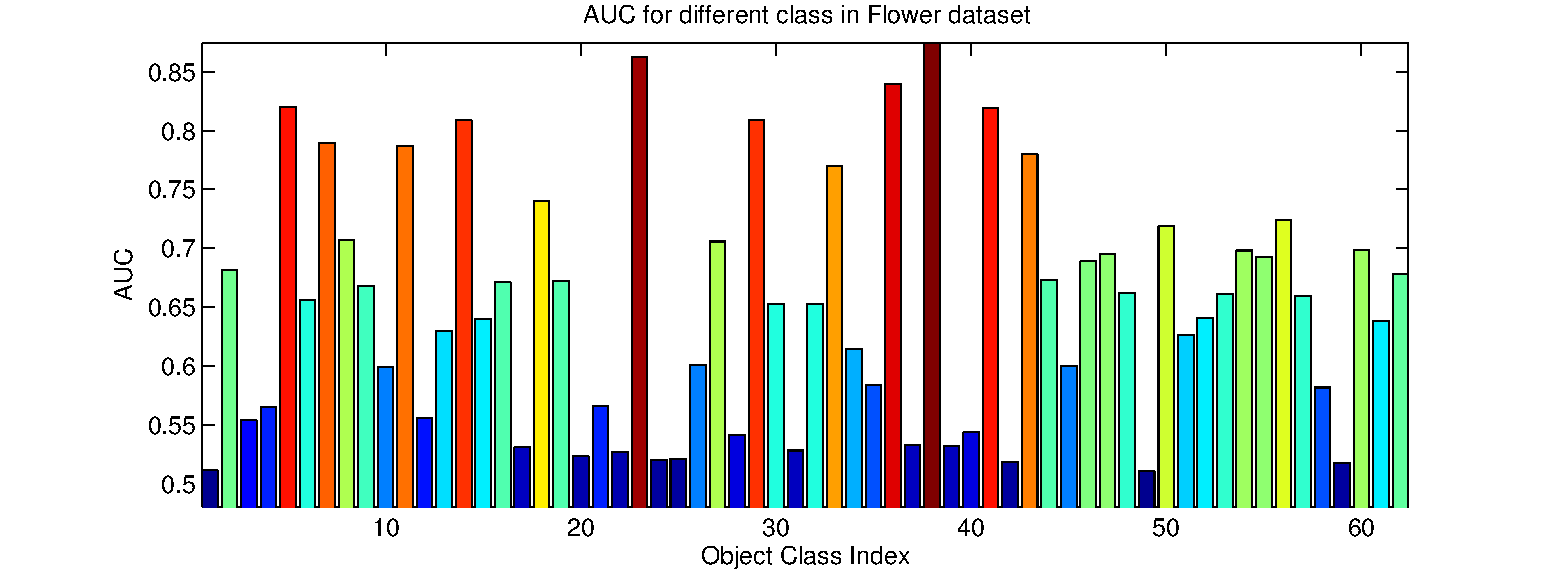
\includegraphics[width=0.6\linewidth,height=.150\linewidth]{fig1auc.eps}
\caption{Kernel: AUC of the 62 unseen classifiers the flower data-sets over three different splits}
\label{F:AUCs}
 \end{minipage}%
\end{figure*}
\end{comment}



\begin{comment}
% This is the good table
\begin{figure*}
  \begin{minipage}[b]{0.25\linewidth}
    \centering
     \captionof{table}{Kernel: MAU on a seen-unseen split-Birds Dataset (MKL)}
\label{tbl:birdsmkl}
    \scalebox{0.55}
  {
\begin{tabular}{|c|c|c|}
\hline 
& MAU & improvement \\ 
\hline 
{SVM-DT kernel-rbf (text)}& \textbf{4.10  \%} &   \\ 
\hline 
Linear Classifier \ignore{Prediction} & 2.74 \% & 49.6 \% \\ 
\hline 
\end{tabular} }
  \centering
   \vspace{2mm}
  \captionof{table}{Kernel: MAU on a seen-unseen split-Birds Dataset (Attributes)} 
\label{tbl:birds3}
    \scalebox{0.6}
  {
\begin{tabular}{|c|c|c|}
\hline 
 & MAU & improvement \\ 
\hline 
{SVM-DT kernel-rbf }& \textbf{5.6  \%} &   \\ 
\hline 
{DT kernel-rbf }& {4.03 \%} &  32.7 \% \\ 
\hline 
Lampert DAP\ignore{  \cite{Lampert09}} & 4.8  \% & 16.6 \% \\ 
\hline 
\end{tabular}}
 \scalebox{0.6}
  {
\begin{tabular}{|c|c|c|}
\hline 
 & Recall & improvement \\ 
\hline 
{SVM-DT kernel-rbf }& \textbf{76.7  \%} &   \\ 
\hline 
Lampert DAP  \ignore{\cite{Lampert09}} & 68.1  \% & 12.6 \% \\ 
\hline 
\end{tabular}
 }
         \vspace{6mm}
\end{minipage}
 \begin{minipage}[b]{0.01\linewidth}$\,$\end{minipage}
  \begin{minipage}[b]{0.27\linewidth}
  \centering
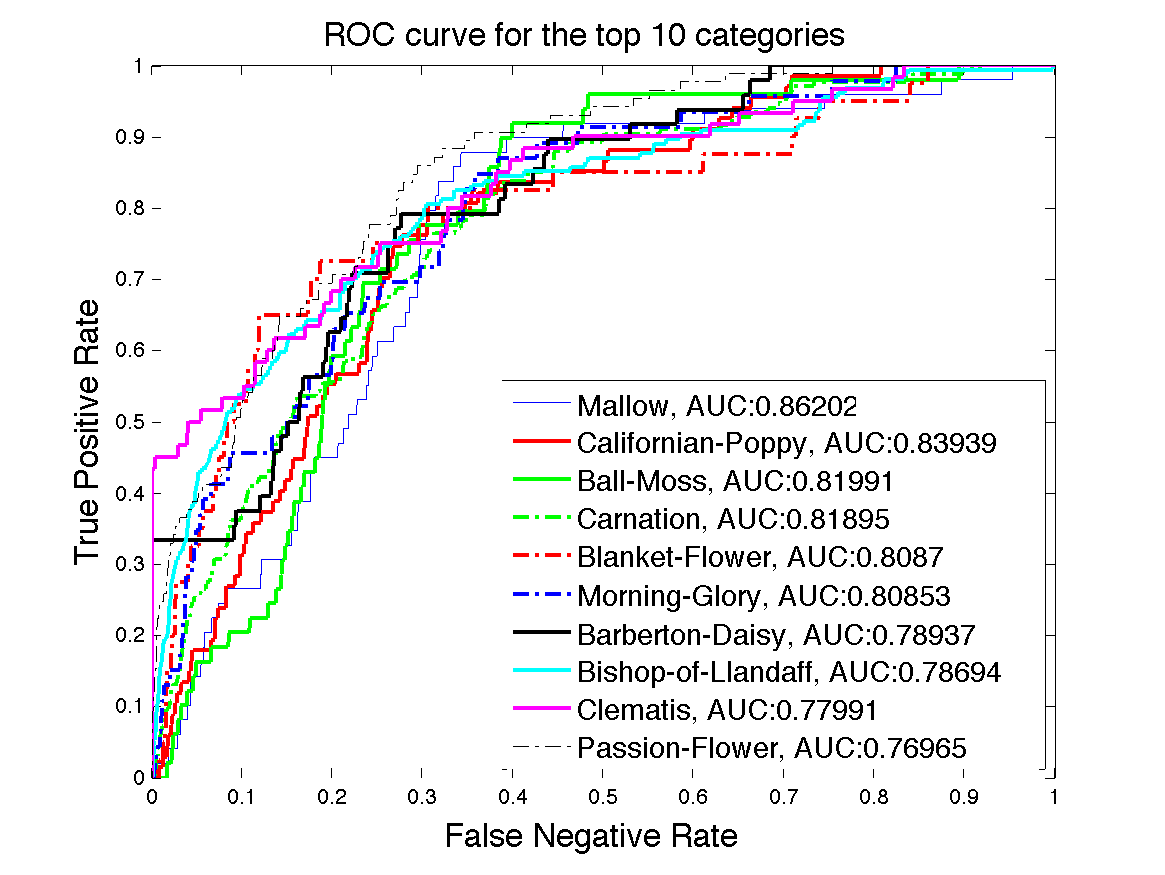
\includegraphics[width=1.0\linewidth,height=.72\linewidth]{figroc.eps}
\caption{ROC-curves for the top 10 classifiers in Flower dataset}
\label{F:top10}
  \end{minipage}%
   \begin{minipage}{0.01\linewidth}$\,$\end{minipage} \begin{minipage}[b]{0.25\linewidth}
   \hspace{-6.8mm}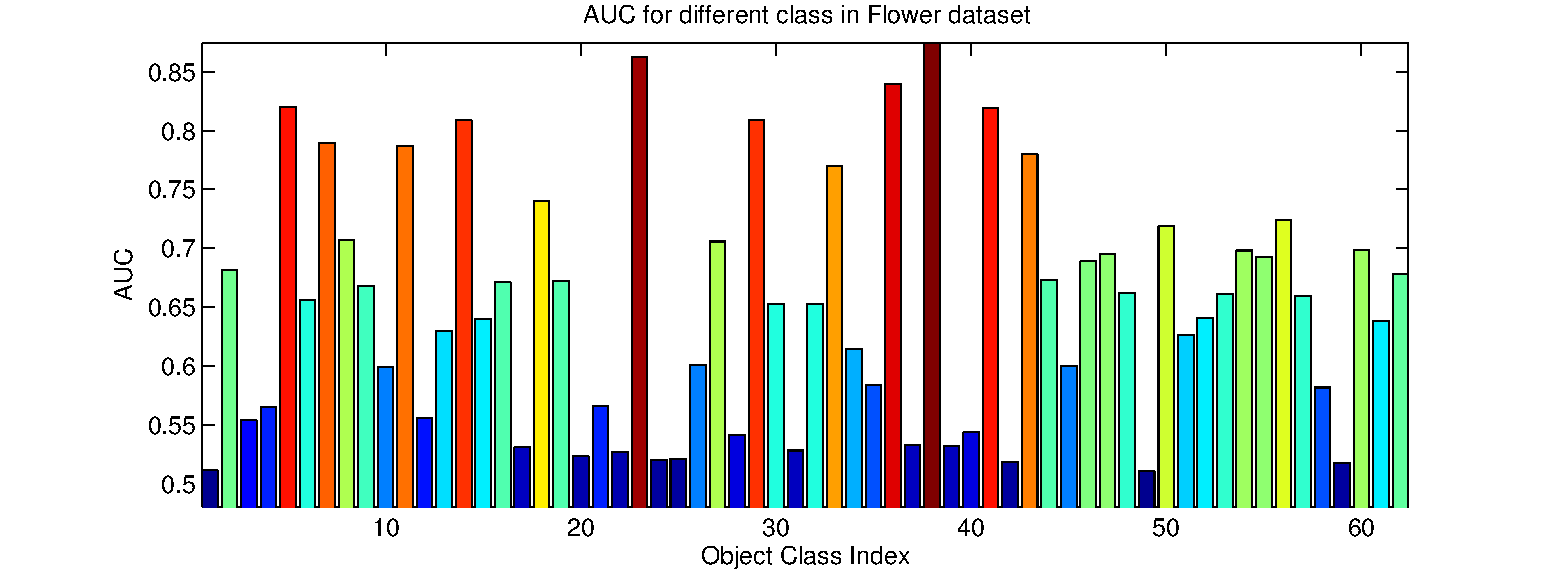
\includegraphics[width=1.15\linewidth,height=.40\linewidth]{fig1auc.eps}
\caption{Kernel: AUC of the 62 unseen classifiers the flower data-sets over three different splits}
\label{F:AUCs}
 \end{minipage}%
\end{figure*}
%\vspace{-10mm}

 \end{comment}

%\textit{Conclusion on textual features as $\mathcal{E}$ space: }
 




 
%\vspace{-5mm}
\begin{comment}
\begin{table}[h!]
\caption{Average AUC of the Unseen classes on three three seen/unseen  splits - Flower Dataset}
\label{tbl:flowerauc}
  \centering
\begin{tabular}{|c|c|c|}
\hline 
 & AUC & improvement \\ 
\hline 
{SVM-DT kernel-rbf }& {0.653 (+/-  0.009) } &   \\ 
\hline 
{DT kernel-rbf }& {0.623 (+/-  0.01) \%} & 4.7 \% \\ 
\hline 
Linear Classifier Prediction & 0.658 (+/-  0.034) & - 0.7 \% \\ 
\hline 
Domain Transfer~\cite{Hoseini13,da11} &0.644 (+/-  0.008) &  1.28 \%\\ 
\hline 
\end{tabular} 
\end{table}


\begin{table}[htbp]
  \centering
  \caption{Average AUC of the Unseen classes on a seen/unseen  split - Birds Dataset }
  \label{tbl:birdsauc}
    \begin{tabular}{|c|c|c|}
  \hline 
 & AUC & improvement \\ \hline 
    SVM-DT kernel-rbf & 0.61  &  \\\hline 
    DT-kernel-rbf & 0.57  & 7.02 \% \\ \hline 
    Linear Classifier Prediction & 0.62  & -1.61\% \\ 
    \hline 
    Domain Transfer~\cite{Hoseini13,da11}  & 0.56  & 8.93\% \\
    \hline 
    \end{tabular}
  \label{tab:addlabel}
\end{table}
\end{comment}



%\vspace{-10mm}
\begin{comment}

\begin{table*}[ht!]
\caption{Multi-class Accuracy of the Unseen classes (MAU)  on a seen-unseen split-Birds Dataset}
\label{tbl:birds}
  \centering
\begin{tabular}{|c|c|c|}
\hline 
& accuracy & improvement \\ 
\hline 
{SVM-DT kernel-rbf }& \textbf{3.4  \%} &   \\ 
\hline 
{DT kernel-rbf }& {2.95  \%} & 15.25 \% \\ 
\hline 
Linear Classifier Prediction& 2.62 \% & 29.77 \% \\ 
\hline 
Domain Transfer~\cite{Hoseini13,da11} & 2.47 \% & 37.65 \% \\ 
\hline 
\end{tabular} 
\end{table*}
\begin{table*}[ht!]
\caption{Multi-class Accuracy of the Unseen classes (MAU)  on three seen/unseen splits - Flower Dataset}
\label{tbl:flower}
  \centering
\begin{tabular}{|c|c|c|}
\hline 
  & accuracy & improvement \\ 
  \hline 
{SVM-DT kernel-rbf }& \textbf{9.1 (+/-  2.77) \%} &   \\ 
\hline 
{DT kernel-rbf }& \textbf{6.64 (+/-  4.1) \%} & 37.93 \% \\ 
\hline 
Linear Classifier Prediction & 5.93  (+/-  1.48)\% & 54.36 \% \\ 
\hline 
Domain Transfer~\cite{Hoseini13,da11} & 5.79 (+/-  2.59)\% & 58.46 \% \\ 
\hline 
\end{tabular} 
\end{table*}
\end{comment}

\subsubsection{Multiple Kernel Learning (MKL) Experiment}

This experiment shows the added value of  proposing a kernelized zero-shot learning approach. We conducted an experiment where the final kernel on the visual domain is produced by Multiple Kernel Learning \cite{MKKLAlgs11}. For the visual domain, we extracted kernel descriptors for Birds dataset. Kernel descriptors provide a principled way to turn any pixel attribute to patch-level features, and are able to generate rich features from various recognition cues. We specifically used four types of kernels introduced by~\cite{bo_nips10} as follows: \textit{Gradient Match Kernels} that captures image variation based on predefined kernels on image gradients. \textit{Color Match Kernel} that describes patch appearance using two kernels on top of RGB and normalized RGB for regular images and intensity for grey images. These kernels capture image variation and visual apperances. For modeling the local shape, \textit{Local Binary Pattern} kernels have been applied. We computed these kernel descriptors on local image patches with fixed size 16 x 16 sampled densely over a grid with step size 8 in a spatial pyramid setting with four layers. The dense features are vectorized using codebooks of size 1000. This process ended up with a 120,000 dimensional feature for each image (30,000 for each type). Having extracted the four types of descriptors, we compute an rbf kernel matrix for each type separately. We learn the bandwidth parameters for each rbf kernel by cross validation on the seen classes. Then, we generate a new kernel \small$k_{mkl}(d, d') = \sum_{i=1}^4 w_i k_i(d, d')$\normalsize, such that $w_i$ is a weight assigned to each kernel. We learn these weights by applying Bucak's Multiple Kernel Learning algorithm \cite{nips10_Bucak}. Then, we applied our approach where the MKL-kernel is used in the visual domain and rbf kernel in the text domain similar to the previous experiments.



 To compare the kernel prediction approach to the linear prediction approach (formulation (E)) under this setting,  we concatenated  all kernel descriptors to end up with  120,000 dimensional feature vector in the visual domain. As highlighted in  the kernel approach section, the linear prediction approach solves a quadratic program of \small$N+d_v+1\,$\normalsize variables for each unseen class.   Due to the large dimensionality of data  (\small$d_v = 120,000$\normalsize), this is not tractable. To make this setting applicable, we reduced the dimensionality of the feature vector into $4000$ using PCA\ignore{ to make it feasible to compute the performance}. This highlights the benefit of our approach since our quadratic program does not depend on the dimensionality of the data. Table ~\ref{tbl:birdsmkl} shows MAU for the kernel prediction approaches under this setting against  linear prediction. The results show the benefits of having a kernel prediction for zero shot learning where kernel methods to construct an arbitrary kernel that  improves the performance.

\subsection{Multiple Representation Experiment and  Distributional Semantic(DS) Kernel}
\label{sec64}

The aim of this experiment is to show that the kernel approach perform on different representations of text $\mathcal{T}$ and visual domains $\mathcal{V}$. In this experiment, we extracted Convolutional Neureal Network(CNN) image features for the Visual domain. We used caffe~\cite{jia2014caffe} implementation of~\cite{imagenetnips12}. Then, we extracted the sixth activation feature of the CNN (FC6) since we found it works the best on the standard classification setting. We found this consistent with the results of~\cite{donahue2014decaf} over different CNN layers. While using  TFIDF feature of text description and CNN features for images, we achieved 2.65\% for the linear version and 4.2\% for the rbf kernel on both text and images. We further improved the performance to 5.35\% by using our proposed Distributional Semantic (DS) kernel in the text domain and rbf kernel for images. In this DS experiment, we used the  distributional semantic model by~\cite{mikolov2013distributed} trained on  GoogleNews corpus (100 billion words)  resulting in a vocabulary of size 3 million words, and word vectors of $K=300$ dimensions. This experiment shows both the value of having a kernel version and also the value of the proposed kernel in our setting. We also applied the zero shot learning approach in~\cite{norouzi2014zero} which performs worse in our settings; see Table~\ref{tbl:birdscnn}. 



\subsubsection{Attributes Experiment}

We emphasis that our  goal from this experiment is not attribute prediction. However, it was interesting for us to see the behavior of our method where $\mathcal{T}$ space is defined from attributes instead of text. In contrast to attribute-based models, which fully utilize attribute information to build attribute classifiers, we do not learn attribute classifiers. In this experiment, our method  uses only the first moment of information of the attributes (i.e. the average attribute vector). We decided to compare to an attribute-based approach from this perspective. In particular, we applied the  (DAP) attribute-based model~\cite{lampertPAMI13,Lampert09}, widely adopted in many applications (\textit{e.g.,} \cite{liu2013video,rohrbach11cvpr}), to the Birds dataset. 




% in our case will not be easily comparable to attribute-based approaches. We argue that the comparison from this perspective will not be conclusive for the following two reasons. 1) if the comparison is not in our favor, that does not role out the value of our work as a step towards a general approach for predicting classifier without explicit attribute definition  2) If the comparison is in our favor, one might argue better results could have been obtained with better attribute definition/learning. 


For this experiment, we compute the average attributes provided with images for each category, without learning any binary classifiers.  We computed this as  \small$\mathcal{T}\,$\normalsize domain representation for the Birds dataset only, since the Flower dataset does not have attributes. Attribute annotation of Birds dataset is provided in terms of: ``Visibility" and ``Certainty". The first term is $1$ if the attribute is visible and $0$ otherwise. The second term indicates how certain the annotator was about his decision with three levels of ``Certain", ``Guessing" and ``probable". We assigned probability of a visible attribute when the annotator is sure about his decision to $1$ and when he is sure of not seeing the attribute to $0$. All other combination of decisions fall in the range of $(0,1)$. As this attribute annotation is provided for each images, we averaged these scores across all the samples of a class to get a single attribute descriptor for each class, to be consistent with our learning setting. For visual domain, we used classeme features in this experiment (as table~\ref{tbl:flowerbirdsmauauc} experiment )\ignore{(as in section ~\ref{exp1} )}. 




%In contrast to attribute-based models, which fully utilize attribute information to build attribute classifiers, our approach do not learn attribute classifiers since we do. \ignore{Also in our approach  attributes are only defined at the class level. In that sense,} Our method also uses only the first moment of information of the attributes (i.e. the average attribute vector). We decided to compare to an attribute-based approach from this perspective. In particular, we applied the  (DAP) attribute-based model \cite{Lampert09,lampertPAMI13}, widely adopted in many applications (\textit{e.g.} \cite{rohrbach11cvpr}), to the Birds dataset.

   
\begin{table}
\centering
 \caption{Kernel: Recall and MAU on a seen-unseen split-Birds Dataset (Attributes)} 
\label{tbl:birds3}
 \vspace{-1mm}
\scalebox{1.0}
  {
\begin{tabular}{|c|c|c|}
\hline 
 & Recall & improvement \\ 
\hline 
{SVM-DT kernel-rbf }& \textbf{76.7  \%} &   \\ 
\hline 
Lampert DAP  {\cite{Lampert09}} & 68.1  \% & 12.6 \% \\ 
\hline 
\end{tabular}
 }

    \scalebox{1.0}
  {
\begin{tabular}{|c|c|c|}
\hline 
 & MAU & improvement \\ 
\hline 
{SVM-DT kernel-rbf }& \textbf{5.6  \%} &   \\ 
\hline 
{DT kernel-rbf }& {4.03 \%} &  32.7 \% \\ 
\hline 
Lampert DAP {  \cite{Lampert09}} & 4.8  \% & 16.6 \% \\ 
\hline 
\end{tabular}}

 \vspace{-2mm}
\end{table}

An interesting result is that our approach achieved $5.6\%$  MAU ($224\%$ the random guess performance); see Table ~\ref{tbl:birds3}. In contrast, we get $4.8\%$ multiclass accuracy using  DAP approach~\cite{lampertPAMI13}. In this setting, we also measured the $N_{sc}$ to $ N_{sc}+1$ average recall. We found the recall measure is $76.7\%$ for our SVM-DT-kernel, while it is $68.1\%$ on  the DAP approach, which reflects better true positive rate (positive class is the unseen one). We find these results interesting, since we achieved it without learning any attribute classifiers, as in~\cite{lampertPAMI13}. When comparing the results  of our approach using attributes (Table~\ref{tbl:birds3}) vs. textual description (Table~\ref{tbl:flowerbirdsmauauc})\footnote{We are refering to the experiment that uses classeme as visual features to have a consistent comparison to here} as the $\mathcal{T}$ space used for prediction, it is clear that the attribute features gives better prediction. This support our hypothesis that the more meaningful the \small$\mathcal{T}\,$\normalsize domain, the better the performance on \small$\mathcal{V}\,$\normalsize domain. This indicates that if a better textual representation is used, a better performance can be achieved. Attributes are a good semantic representation of a class but it is difficult to  define attributes for an arbitrary class and further measure the confidence of each one. In contrast, it is much easier to find an unstructured  text description for visual class. 


%In this experiment, we compare our approach with an attribute-based approach~\cite{Lampert09} on Birds dataset, for the purpose argued earlier in this section. 
%Table~\ref{tbl:birds3} shows the results of this experiment. 
%An interesting result is that our approach achieved $5.6\%$  MAU ($224\%$ the random guess performance) \ignore{($36.36\%$ of the multiclass accuracy of seen classes (i.e. $15.4\%$))}. In contrast, we get $4.8\%$ multiclass accuracy using  DAP approach~\cite{Lampert09}. In this setting, we also measured the $N_{sc}$ to $ N_{sc}+1$ average recall. We found the recall measure is $76.7\%$ for our SVM-DT-kernel, while it is $68.1\%$ on  the DAP approach, which reflects better true positive rate (positive class is the unseen one). We find these results interesting, since we achieved it without learning any attribute classifiers, as in~\cite{Lampert09}. 
%\vspace{-5mm}
%\vspace{-5mm}

%When comparing the results  of our approach using attributes (Table~\ref{tbl:birds3}) vs. textual description (Table~\ref{tbl:flowerbirdsmauauc})\footnote{We are refering to the experiment that uses classeme as visual features to have a consistent comparison} as $\mathbb{T}$ space, it is clear that the attribute features gives better prediction. This support our hypothesis that the more meaningful the \small$\mathcal{T}\,$\normalsize domain, the better the performance on \small$\mathcal{V}\,$\normalsize domain. This is since, the domain transfer function better captures the correlation between \small$\mathcal{T}\,$\normalsize and \small$\mathcal{V}\,$\normalsize domains in this case. This indicates that if a better textual representation is used, a better performance can be achieved. Attributes are a good semantic representation of a class but it is difficult to  define attributes for an arbitrary class and further measure the confidence of each one. In contrast, it is much easier to find a text description for class. 










\section{Conclusion}
We explored the problem of predicting visual classifiers from textual description of classes with no training images.  We investigated and  experimented with different formulations for the problem within the fine-grained categorization context.  We first proposed  a novel formulation that captures information between the visual and textual domains by involving knowledge transfer from textual features to visual features, which indirectly leads to predicting a linear visual classifier described by the text. \ignore{In the future, we are planning to propose a kernel version to tackle the problem instead of using linear classifiers. Furthermore, } We also proposed a new zero-shot learning technique to predict kernel-classifiers of unseen categories using information from a privilege space. We formulated the problem as domain transfer function from text description  to the visual classification space, while supporting kernels in both domains. We proposed a one-class SVM adjustment to our domain transfer function in order to improve the prediction. We validated the performance of our model by several experiments. We also showed that   our approach using with weak-attributes. We illustrated the value of proposing a kernelized version by applying kernels generated by Multiple Kernel Learning (MKL) and achieved better results.  \ignore{We  compared our approach with  state-of-the-art approaches and interesting findings have been reported.} In the future, we aim to improve this model by learning the unseen classes jointly and on a larger scale. %We will study predicting classifiers.   \ignore{We also plan to further scale up the proposed model to address very large number of categories ( $>$ 1000).} 

\ignore{
We are also looking forward to studying more features for the $\mathcal{X}$ and $\mathcal{E}$ domains in a  large scale setting (number of classes $>$ 1000). }



% use section* for acknowledgement
%\section*{Acknowledgment}
\noindent \textbf{Acknowledgment. } This research was partially funded by NSF award IIS-1218872 and IIS-1409683. 

%The authors would like to thank...


% Can use something like this to put references on a page
% by themselves when using endfloat and the captionsoff option.
\ifCLASSOPTIONcaptionsoff
  \newpage
\fi



% trigger a \newpage just before the given reference
% number - used to balance the columns on the last page
% adjust value as needed - may need to be readjusted if
% the document is modified later
%\IEEEtriggeratref{8}
% The "triggered" command can be changed if desired:
%\IEEEtriggercmd{\enlargethispage{-5in}}

% references section

% can use a bibliography generated by BibTeX as a .bbl file
% BibTeX documentation can be easily obtained at:
% http://www.ctan.org/tex-archive/biblio/bibtex/contrib/doc/
% The IEEEtran BibTeX style support page is at:
% http://www.michaelshell.org/tex/ieeetran/bibtex/
%\bibliographystyle{IEEEtran}
% argument is your BibTeX string definitions and bibliography database(s)
%\bibliography{IEEEabrv,../bib/paper}
%
% <OR> manually copy in the resultant .bbl file
% set second argument of \begin to the number of references
% (used to reserve space for the reference number labels box)
%\begin{thebibliography}{1}
%
%\bibitem{IEEEhowto:kopka}
%H.~Kopka and P.~W. Daly, \emph{A Guide to \LaTeX}, 3rd~ed.\hskip 1em plus
%  0.5em minus 0.4em\relax Harlow, England: Addison-Wesley, 1999.
%
%\end{thebibliography}

% biography section
% 
% If you have an EPS/PDF photo (graphicx package needed) extra braces are
% needed around the contents of the optional argument to biography to prevent
% the LaTeX parser from getting confused when it sees the complicated
% \includegraphics command within an optional argument. (You could create
% your own custom macro containing the \includegraphics command to make things
% simpler here.)
%\begin{IEEEbiography}[{\includegraphics[width=1in,height=1.25in,clip,keepaspectratio]{mshell}}]{Michael Shell}
% or if you just want to reserve a space for a photo:

%\begin{IEEEbiography}{Mohamed Elhoseiny}
%is a PhD student at the Department
%of Computer Science, Rutgers, the State University of New Jersey. He is also a member of the Center for Computational Biomedicine Imaging and Modeling (CBIM). He is currently pursuing his studies in computer vision and multimedia
%as a PhD student in the Computer Science department at Rutgers University.
%\end{IEEEbiography}
%
%% if you will not have a photo at all:
%
%\begin{IEEEbiography}{Ahmed Elgammal}
%is an associate professor at the Department
%of Computer Science, Rutgers, the State University of
%New Jersey Since Fall 2002. Dr. Elgammal is also a member of
%the Center for Computational Biomedicine Imaging and Modeling
%(CBIM). His primary research interest is computer vision
%and machine learning. His research focus includes human activity
%recognition, human motion analysis, tracking, human identification, and statistical
%methods for computer vision. Dr. Elgammal received the National Science Foundation
%CAREER Award in 2006. Dr. Elgammal has been the Principal Investigator and
%Co-Principal Investigator of several research projects in the areas of Human Motion
%Analysis, Gait Analysis, Tracking, Facial Expression Analysis and Scene Modeling;
%funded by NSF and ONR. Dr. Elgammal is Member of the review committee/board
%in several of the top conferences and journals in the computer vision field. Dr. Elgammal
%received his Ph.D. in 2002 from the University of Maryland, College Park. He is
%a senior IEEE member.
%\end{IEEEbiography}


%
%\begin{IEEEbiography}{Babak Saleh}
%Biography text here.
%\end{IEEEbiography}
%
%\begin{IEEEbiographynophoto}{John Doe}
%Biography text here.
%\end{IEEEbiographynophoto}

% insert where needed to balance the two columns on the last page with
% biographies
%\newpage



% You can push biographies down or up by placing
% a \vfill before or after them. The appropriate
% use of \vfill depends on what kind of text is
% on the last page and whether or not the columns
% are being equalized.

%\vfill

% Can be used to pull up biographies so that the bottom of the last one
% is flush with the other column.
%\enlargethispage{-5in}

{
%\bibliographystyle{ieee}
%\bibliography{egbib2}
\bibliographystyle{IEEEtran}
\bibliography{egbib,write_a_classifier,elgammal,NLPVision,NLPVisionProposal,smara}
}
%\vspace{-13mm}
%\begin{IEEEbiographynophoto}{Mohamed Elhoseiny}
%Mohamed Elhoseiny is a PhD Candidate at Rutgers is a PhD student at the Department of Computer Science. He is also a member of the Center for Computational Biomedicine Imaging and Modeling (CBIM). He received a MSc degree from Rutgers in 2014. His primary research interest is Language\&Vision, multi-view, and multimodal learning (PhD focus). 
%%as a PhD student in the Computer Science department at Rutgers University.
%\end{IEEEbiographynophoto}
%\vspace{-13mm}
%\begin{IEEEbiographynophoto}{Ahmed Elgammal}
%is an associate professor at the Department
%of Computer Science, Rutgers, the State University of New Jersey Since Fall 2002. Dr. Elgammal
%received his Ph.D. in 2002 from the University of Maryland, College Park. He is a senior IEEE member.
%\end{IEEEbiographynophoto}
%\vspace{-13mm}
%\begin{IEEEbiographynophoto}{Babak Saleh} is a PhD student at Rutgers University, Computer Science department. His primary interests is Computer vision focusing on abnormality detection and modeling artist influence from paintings.  
%\end{IEEEbiographynophoto}
%\vspace{10mm}
% that's all folks
\end{document}


